%%%%%%%%%%%%%%%%%%%%%%%%%%%%%%%%%%%%%%
\documentclass[aspectratio=169, xcolor={dvipsnames,svgnames}]{beamer}
\mode<presentation> {

% The Beamer class comes with a number of default slide themes
% which change the colors and layouts of slides. Below this is a list
% of all the themes, uncomment each in turn to see what they look like.

%\usetheme{default}
%\usetheme{AnnArbor}
%\usetheme{Antibes}
%\usetheme{Bergen}
%\usetheme{Berkeley}
%\usetheme{Berlin}
%\usetheme{Boadilla}
%\usetheme{CambridgeUS}
%\usetheme{Copenhagen}
%\usetheme{Darmstadt}
%\usetheme{Dresden}
%\usetheme{Frankfurt}
%\usetheme{Goettingen} %intersing
%\usetheme{Hannover}
%\usetheme{Ilmenau}
%\usetheme{JuanLesPins}
%\usetheme{Luebeck}
\usetheme{Madrid}   %default
%\usetheme{Malmoe}
%\usetheme{Marburg}
%\usetheme{Montpellier}
%\usetheme{PaloAlto}
%\usetheme{Pittsburgh}
%\usetheme{Rochester}
%\usetheme{Singapore}
%\usetheme{Szeged}
%\usetheme{Warsaw}

% As well as themes, the Beamer class has a number of color themes
% for any slide theme. Uncomment each of these in turn to see how it
% changes the colors of your current slide theme.

%\usecolortheme{albatross}
%\usecolortheme{beaver} %https://www.overleaf.com/project/5d747c71ac3a15000125da4f
%\usecolortheme{beetle}
%\usecolortheme{crane}
%\usecolortheme{dolphin}
%\usecolortheme{dove}
%\usecolortheme{fly}
%\usecolortheme{lily}
%\usecolortheme{orchid}
%\usecolortheme{rose}
%\usecolortheme{seagull}
%\usecolortheme{seahorse}
%\usecolortheme{whale}
\usecolortheme{wolverine}

%\setbeamertemplate{footline} % To remove the footer line in all slides uncomment this line
\setbeamertemplate{footline}[page number] % To replace the footer line in all slides with a simple slide count uncomment this line

\setbeamertemplate{navigation symbols}{} % To remove the navigation symbols from the bottom of all slides uncomment this line
}

% These are my colors -- there are many like them, but these ones are mine.
% \definecolor{blue}{RGB}{0,114,178}
% \definecolor{red}{RGB}{213,94,0}
% \definecolor{yellow}{RGB}{240,228,66}
% \definecolor{green}{RGB}{0,158,115}

\usepackage{multicol}
\usepackage{graphicx} % Allows including images
\usepackage{booktabs} % Allows the use of \toprule, \midrule and \bottomrule in tables
\usepackage{amsmath, amssymb, amsthm, array,xfrac, mathrsfs}
\usefonttheme[onlymath]{serif} % To make math cursive
\usepackage{gensymb}
\usepackage{physics} % for partial and derivative
\usepackage[tikz]{mdframed}
\usetikzlibrary{decorations.pathreplacing,angles,quotes, fadings}
\usetikzlibrary{trees,positioning,arrows,fit,shapes,calc}
% Draw cross or circle in tikz environment
\usetikzlibrary{shapes.misc}
%\usepackage[shortlabels]{enumitem}
\usepackage{empheq}
\usepackage[makeroom]{cancel}
% Clickable Links
\usepackage{hyperref}
\usepackage{siunitx}
\usepackage{venndiagram}
% CAPTION
\usepackage{caption}
\captionsetup{justification=centering}
\usepackage{epigraph}
\usepackage{tikz,tikz-3dplot} 
\usepackage{fouriernc}

\usepackage{pgfpages}
%\pgfpagesuselayout{resize to}[a4paper,landscape] %To rescale to A4

%%%%%%%%%%%%%%%%%%%%%%%%%%%%%%%%%%%%%%%
% EXAMPLE COUNTING
%%%%%%%%%%%%%%%%%%%%%%%%%%%%%%%%%%%%%%%
\setbeamertemplate{theorem}[ams style]
\setbeamertemplate{theorems}[numbered]
\makeatletter
\def\@firstoffive#1#2#3#4#5{#1}%
\newenvironment{example*}[1][\relax]
  {\begingroup\ifx#1\relax% No optional argument
   \else% Optional argument given
     \@ifundefined{r@#1}{}{%
       \protected@edef\cont@example@num{\csname r@#1\endcsname}%
       \expandafter\edef\expandafter\cont@example@num\expandafter
         {\expandafter\@firstoffive\cont@example@num}%%
       \renewcommand{\thetheorem}{\cont@example@num}}%
   \fi\addtocounter{theorem}{-1}% Revert to previous theorem count
   \example}
  {\endexample\endgroup}
\makeatother

%%%%%%%%%%%%%%%%%%%%%%%%%%%%%%%%%%%%%%%
% UPPER CASE TITLE
%%%%%%%%%%%%%%%%%%%%%%%%%%%%%%%%%%%%%%%
% \usepackage{textcase,regexpatch}

% \setbeamertemplate{frametitle}{
%   \makeatletter
%   \regexpatchcmd{\insertframetitle}
%     {(\c{usebeamertemplate}.*)\c{fi}}
%     {\c{NoCaseChange}\cB\{\1\cE\}\c{fi}}
%     {}{}%
%   \makeatother
%   \MakeTextUppercase{\insertframetitle}
% }
%%%%%%%%%%%%%%%%%%%%%%%%%%%%%%%%%%%%%%%
% REMOVING PART I, II in \partpart
%%%%%%%%%%%%%%%%%%%%%%%%%%%%%%%%%%%%%%%
\setbeamertemplate{part page}{
        \begin{beamercolorbox}[sep=8pt,center,wd=\textwidth]{part title}
            \usebeamerfont{part title}\insertpart\par
        \end{beamercolorbox}
}
%%%%%%%%%%%%%%%%%%%%%%%%%%%%%%%%%%%%%%%
% RESET TOC NUMBERING FOR EACH PART
%%%%%%%%%%%%%%%%%%%%%%%%%%%%%%%%%%%%%%%
\makeatletter
\AtBeginPart{%
  \beamer@tocsectionnumber=0\relax
  \setcounter{section}{0}
  %\frame{\partpage}%
}
\makeatother

%%%%%%%%%%%%%%%%%%%%%%%%%%%%%%%%%%%%%%%
% CHANGE FIGURE CAPTION NAME
%%%%%%%%%%%%%%%%%%%%%%%%%%%%%%%%%%%%%%%
%\renewcommand{\figurename}{Fig.}

%%%%%%%%%%%%%%%%%%%%%%%%%%%%%%%%%%%%%%%
% TRANSITION FRAME FOR PARTS
%%%%%%%%%%%%%%%%%%%%%%%%%%%%%%%%%%%%%%%
%% Change the bg color to adjust your transition slide background color!
\newenvironment{transitionframe}{
\usebackgroundtemplate{%
\tikz[overlay,remember picture] \node[at=(current page.center)] {
\includegraphics[height=\paperheight,width=\paperwidth]{background/bg.jpg}};
}
\setbeamertemplate{footline}{}
\begin{frame}}{\end{frame}
%\usebackgroundtemplate{ }
}

%%%%%%%%%%%%%%%%%%%%%%%%%%%%%%%%%%%%%%%
% X mark
%%%%%%%%%%%%%%%%%%%%%%%%%%%%%%%%%%%%%%%

\usepackage{pifont}
\newcommand{\xmark}{\text{\ding{55}}}

%%%%%%%%%%%%%%%%%%%%%%%%%%%%%%%%%%%%%%%%%%%%%%%
%           TRUE or FALSE
%%%%%%%%%%%%%%%%%%%%%%%%%%%%%%%%%%%%%%%%%%%%%%%
\newcommand{\true}{\alert{\textbf{T}}}
\newcommand{\false}{\alert{\textbf{F}}}
%%%%%%%%%%%%%%%%%%%%%%%%%%%%%%%%%%%%%%%%%%%%%%%
%  Coloring a row
%%%%%%%%%%%%%%%%%%%%%%%%%%%%%%%%%%%%%%%%%%%%%%%
\usepackage{colortbl}
\definecolor{Gray}{gray}{0.9}
\definecolor{LightCyan}{rgb}{0.88,1,1}
\definecolor{LightBlue}{rgb}{173,216,230}
\definecolor{Amethyst}{rgb}{0.6, 0.4, 0.8}
\usepackage[first=0,last=9]{lcg}
\newcommand{\ra}{\rand0.\arabic{rand}}
\title[Chapter 8]{Geometry} % The short title appears at the bottom of every slide, the full title is only on the title page

\author{Aiden Azarnoush} % Your name
\institute[SPC] % Your institution as it will appear on the bottom of every slide, may be shorthand to save space
{
% St. Petersburg College \\ % Your institution for the title page
% \medskip
\textit{aiden-azarnoush@outlook.com} % Your email address
}
\date{Fall 2021} % Date, can be changed to a custom date

\begin{document}
%%%%%%%%%%%%%%%%%%%%%%%%%%%%%%%%%%%%%%%
%        TITLE FRAME
%%%%%%%%%%%%%%%%%%%%%%%%%%%%%%%%%%%%%%%
\begin{frame}
\titlepage % Print the title page as the first slide
\end{frame}


% PART 1 (SECTION 8.1)
\part{Section 8.1}
%%%%%%%%%%%%%%%%%%%%%%%%%%%%%%%%%%%%%%%
\begin{transitionframe}
    \begin{center}
    { 
        \Huge \textcolor{white}{\textbf{Points, Lines, Planes, and Angles}}
        \\[-1em]
        \noindent\textcolor{white}{\rule{12cm}{0.4pt}}
        
        %\large \textcolor{white}{Section 8.1}
    }
    \end{center}
\end{transitionframe}
%%%%%%%%%%%%%%%%%%%%%%%%%%%%%%%%%%%%%%%
%        SLIDE 1 
%%%%%%%%%%%%%%%%%%%%%%%%%%%%%%%%%%%%%%%
\begin{frame}{Outline}
    \begin{multicols}{2}
        \tableofcontents[part=1, subsubsectionstyle=hide]
    \end{multicols}
\end{frame}
%%%%%%%%%%%%%%%%%%%%%%%%%%%%%%%%%%%%%%%
%        SLIDE 
%%%%%%%%%%%%%%%%%%%%%%%%%%%%%%%%%%%%%%%
\section{History}
\subsection{Ancient Greece}
\begin{frame}{Ancient Greece}
\begin{columns}[c]

\column{.5\textwidth} % Left column and width
\begin{itemize}
    \item Start from Ancient Greece
    \item  $\underbrace{Geo}_{Earth} + \underbrace{metry}_{measurement}$
    \item Euclid developed the discipline in geometry making it a concrete and organized study.
    \item Euclid is considered as a ``Father of Geometry''.
    \item His famous book is called ``Elements''. 
    \item In geometry, we study lines, shapes, surfaces, volumes and their relationships. 
\end{itemize}
\column{.5\textwidth} % Right column and width
    \begin{figure}
        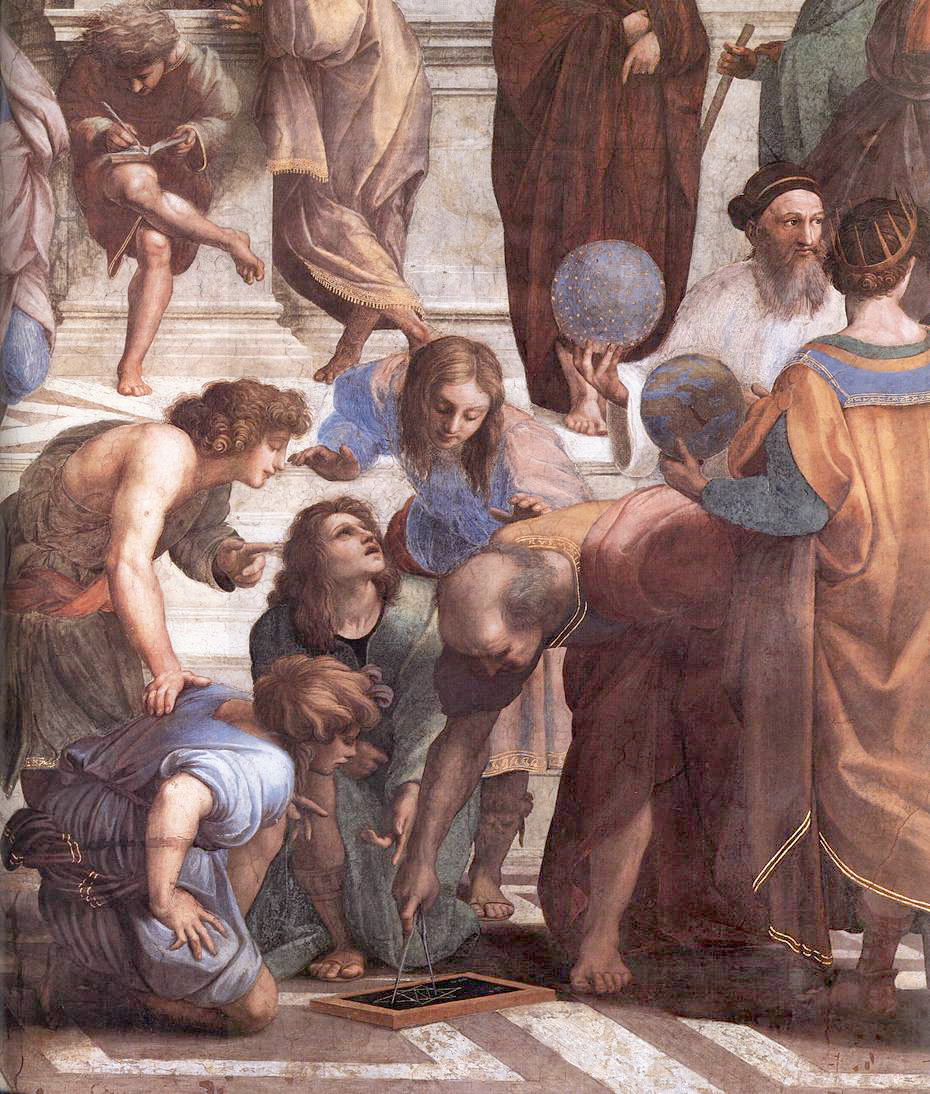
\includegraphics[scale=0.6]{pics/greece.jpg}
    \end{figure}
    %
\end{columns}
\end{frame}
%%%%%%%%%%%%%%%%%%%%%%%%%%%%%%%%%%%%%%
\usebackgroundtemplate{%
\tikz[overlay,remember picture] \node[opacity=0.3, at=(current page.center)] {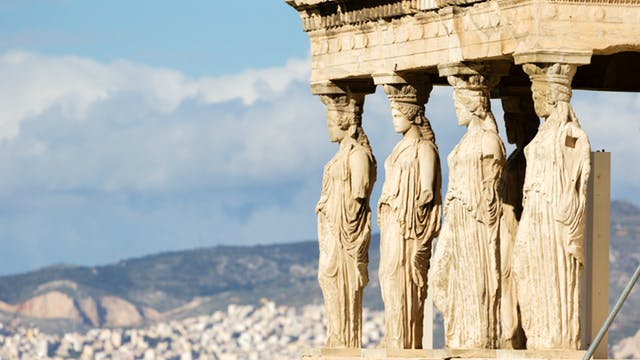
\includegraphics[height=\paperheight,width=\paperwidth]{pics/back.jpg}};
}
%%%%%%%%%%%%%%%%%%%%%%%%%%%%%%%%%%%%%%%
%        SLIDE 
%%%%%%%%%%%%%%%%%%%%%%%%%%%%%%%%%%%%%%%
\subsection{Why should we learn Geometry?}
\begin{frame}{Why should we learn Geometry?}
\begin{itemize}    
    \item Daily life: Brain Calculation, Installing wallpaper, Any measurement at house, Parallel parking, and so on.
    \item Nowadays we used Geometry in: 
        \begin{itemize}    
            \item Arts
            \item Astronomy
            \item Engineering
            \item Drafting
            \item Geology
            \item Architecture
            \item $\ \vdots$
        \end{itemize}
    \item Helpful for: 
        \begin{itemize}
            \item Improving analyzing skills
            \item problem-solving skills
            \item deductive reasoning
            \item $\ \vdots$
        \end{itemize}
\end{itemize}

\end{frame}
%%%%%%%%%%%%%%%%%%%%%%%%%%%%%%%%%%%%%%
\usebackgroundtemplate{ }% undeclare it
%%%%%%%%%%%%%%%%%%%%%%%%%%%%%%%%%%%%%%%
%        SLIDE 
%%%%%%%%%%%%%%%%%%%%%%%%%%%%%%%%%%%%%%%
\section{Different Types of Geometries}
\begin{frame}{Different Types of Geometries}
    \begin{figure}[H]
        \centering
        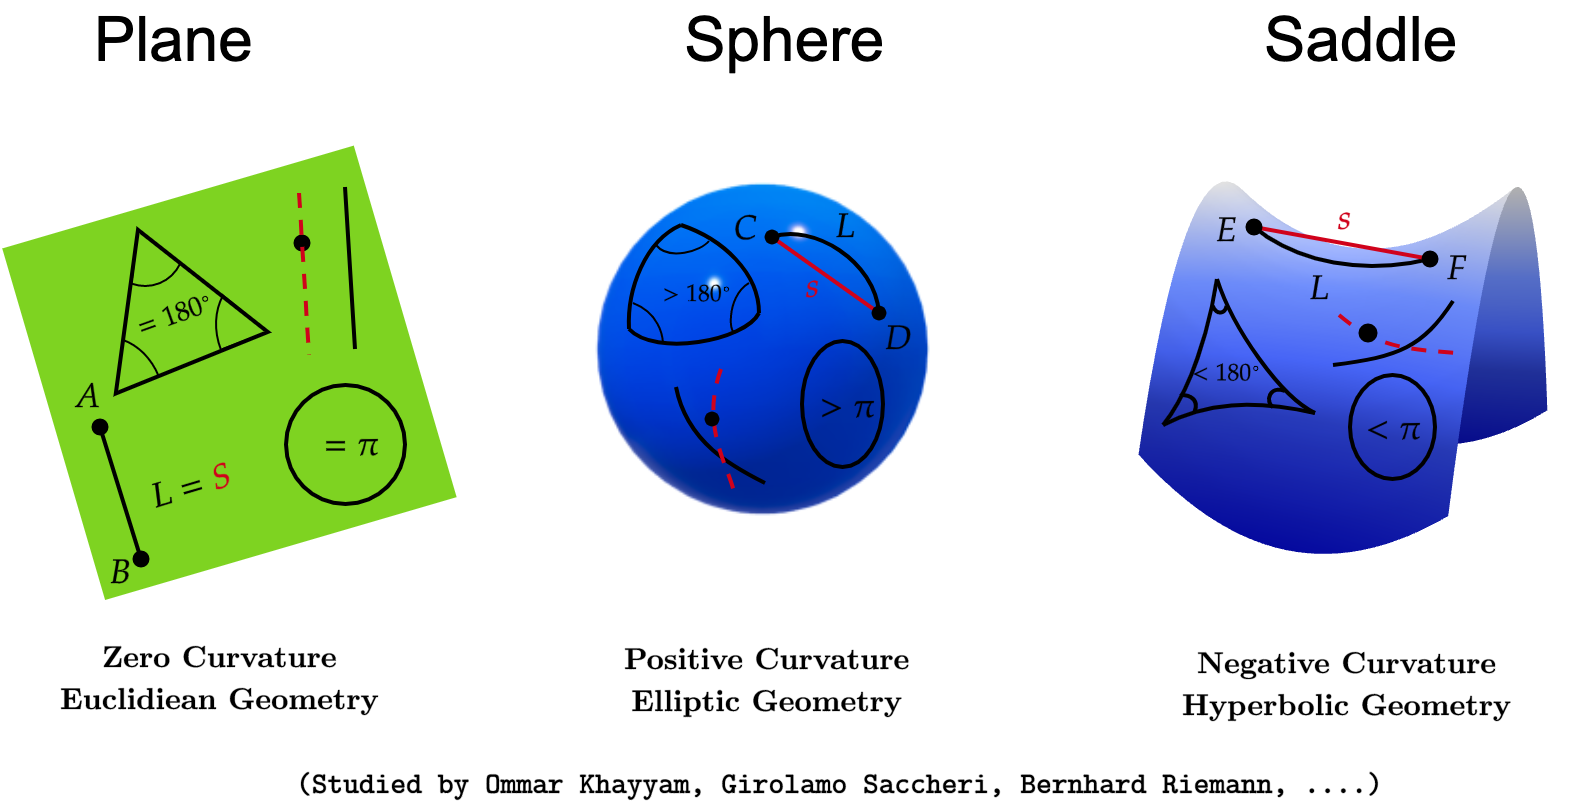
\includegraphics[width=0.8\textwidth]{pics/Euclid_vs_non_Euclid.png}
    \end{figure}
\end{frame}
%%%%%%%%%%%%%%%%%%%%%%%%%%%%%%%%%%%%%%%
%        SLIDE 
%%%%%%%%%%%%%%%%%%%%%%%%%%%%%%%%%%%%%%%
\section{Lines}
\begin{frame}{Lines}
    \begin{block}{Definition}
    \begin{itemize}
        \item  A line is a set of points (points are labeled with capital letters). 
        \item  In other words, a line is
        \setbeamertemplate{items}[triangle]
                    \begin{itemize}
                        \item straight (no bends)
                        \item and extend in both directions without end (infinitely)
                    \end{itemize}
        \setbeamertemplate{items}[default]
    \end{itemize}
    \end{block}
    %
    \begin{figure}[H]
        \centering
        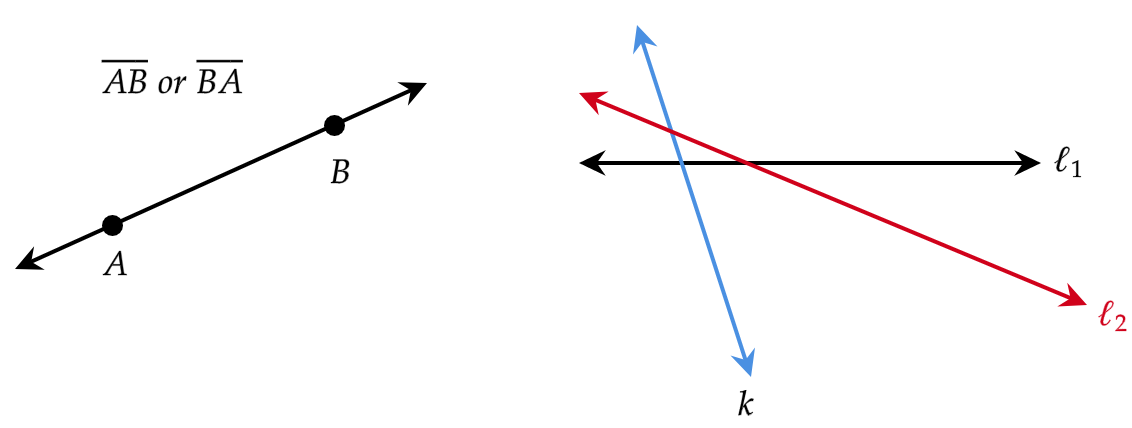
\includegraphics[scale=0.25]{pics/lines.png}
    \end{figure}
\end{frame}
%%%%%%%%%%%%%%%%%%%%%%%%%%%%%%%%%%%%%%%
%        SLIDE 
%%%%%%%%%%%%%%%%%%%%%%%%%%%%%%%%%%%%%%%
\subsection{Parallel Lines}
\begin{frame}{Parallel Lines}
    \begin{itemize}
        \item Lines are parallel if they are always the same distance apart and will never meet.
    \end{itemize}
    %
    \begin{figure}[H]
        \centering
        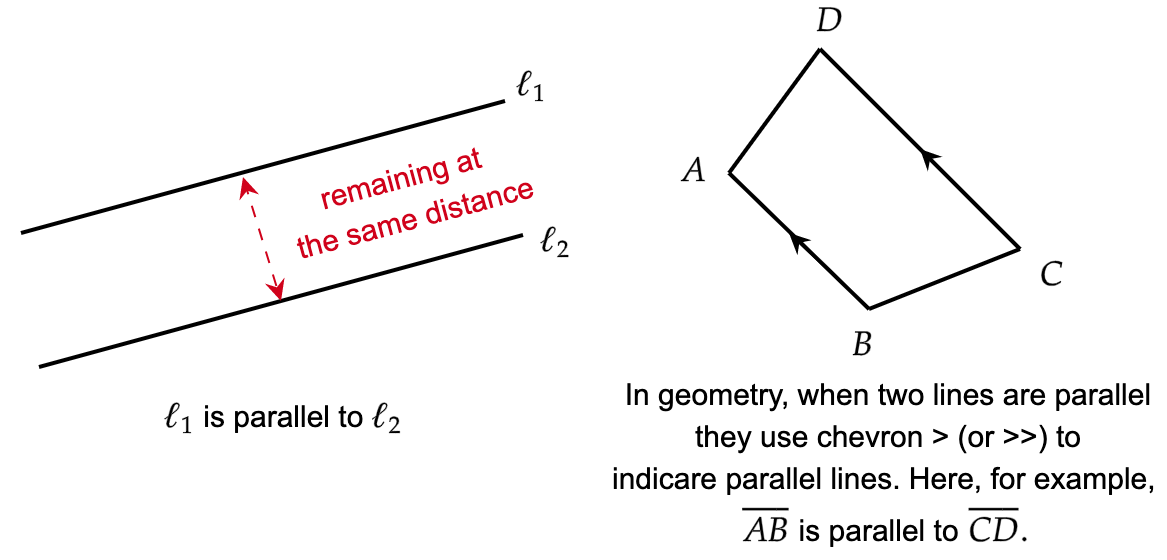
\includegraphics[scale=0.3]{pics/parallel_lines.png}
    \end{figure}
\end{frame}
%%%%%%%%%%%%%%%%%%%%%%%%%%%%%%%%%%%%%%%
%        SLIDE 
%%%%%%%%%%%%%%%%%%%%%%%%%%%%%%%%%%%%%%%
\subsection{Ray}
\begin{frame}{Ray}
    \begin{itemize}
        \item A part of a line that has one endpoint and goes on infinitely in one direction.
        \item A ray can be named using its endpoint first and then any other point on the ray.
    \end{itemize}
    %
    \begin{figure}[H]
        \centering
        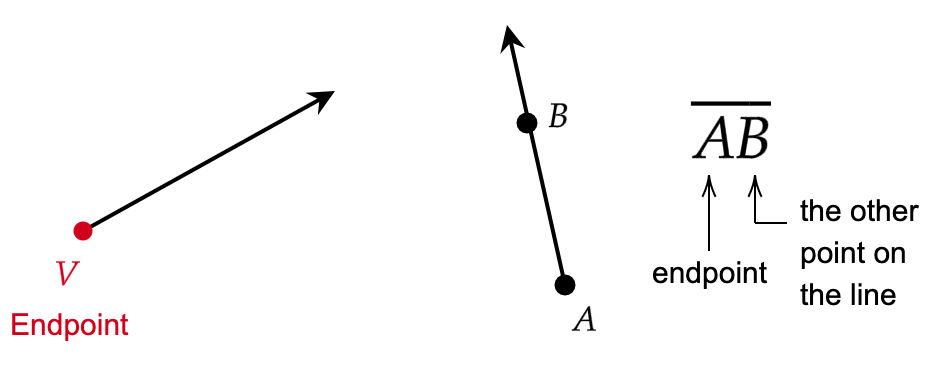
\includegraphics[scale=0.35]{pics/ray.png}
    \end{figure}
\end{frame}
%%%%%%%%%%%%%%%%%%%%%%%%%%%%%%%%%%%%%%%
%        SLIDE 
%%%%%%%%%%%%%%%%%%%%%%%%%%%%%%%%%%%%%%%
\section{Planes}
\begin{frame}[t]{Planes}
    \begin{columns}[c]
    \column{0.5\textwidth}
    \begin{block}{Definition}
    \begin{itemize}
        \item A plane is a two-dimensional surface that extends infinitely in both directions, like an infinitely large white board.
    \end{itemize}
    \end{block}
    %
    \footnotesize{
    \textbf{Some Properties of Planes}
    \begin{itemize}
        \item Any three points that are not on the same line (noncollinear points) determine a unique plane.
        \item The intersection of two distinct planes is a line.
        \item Any line and a point not on the line determine a unique plane.
        \item A line in a plane divides the plane into three parts, the line itself and two half planes.
        \item Two planes that do not intersect are said to be \textit{parallel planes}.
    \end{itemize}}
    %
    \column{0.45\textwidth}
    \begin{figure}
        \centering
        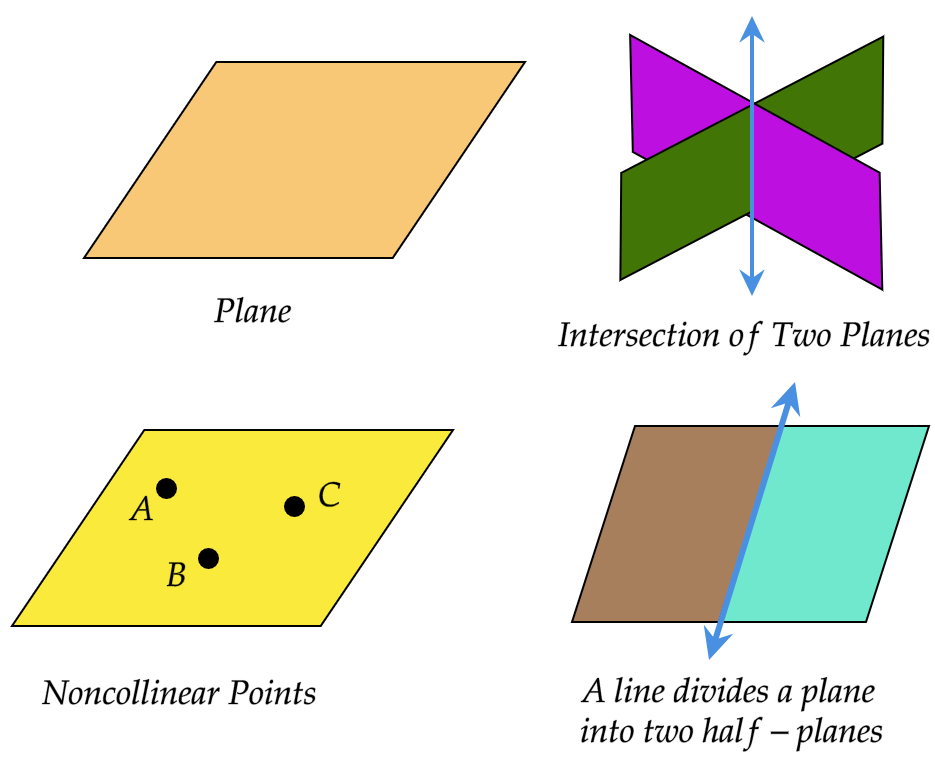
\includegraphics[scale=0.18]{pics/planes.png}
    \end{figure}
    \end{columns}
\end{frame}
%%%%%%%%%%%%%%%%%%%%%%%%%%%%%%%%%%%%%%%
%        SLIDE 
%%%%%%%%%%%%%%%%%%%%%%%%%%%%%%%%%%%%%%%
\section{Angles}
\begin{frame}[t]{Angles}
    \begin{block}{Definition}
    \begin{itemize}
        \item Two rays with a common endpoint form an angle.
        \item The common end point is called vertex.
        \item An angle is the amount of rotation from one ray to the other ray.
        \item Angle is denoted as $\angle $
    \end{itemize}
    \end{block}
    %
    \begin{figure}[H]
    \centering
    \usetikzlibrary{quotes,angles}
    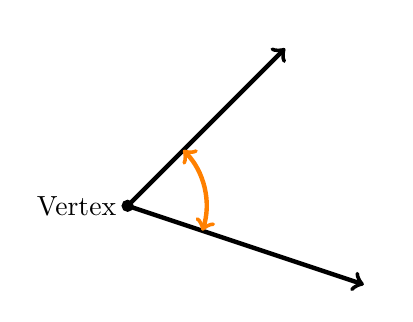
\begin{tikzpicture}
      \fill[black] (0,0)  circle[radius=2pt]; 
      \draw (0,0)  circle[radius=2pt]; 
      %
      \draw[ultra thick,<->]
        (3,-1) coordinate (a) node[right] {}
        -- (0,0) coordinate (b) node[left] {Vertex}
        -- (2,2) coordinate (c) node[above right] {}
        pic[draw=orange, ultra thick, <->, angle eccentricity=1.2, angle radius=1cm]
        {angle=a--b--c};
    \end{tikzpicture}
    \end{figure}
\end{frame}
%%%%%%%%%%%%%%%%%%%%%%%%%%%%%%%%%%%%%%%
%        SLIDE 
%%%%%%%%%%%%%%%%%%%%%%%%%%%%%%%%%%%%%%%
\subsection{How to Name an Angle?}
\begin{frame}[t]{How to Name an Angle?}
    Angles can be named in 3 ways:
    \small{
    \begin{enumerate}
        \item \textbf{Point-Vertex-Point}: The angle is names from a point on one ray, the vertex, and a point on the other ray. This is the most common way to name an angle.
        \item \textbf{Vertex method}: In case where it is not ambiguous, an angle can be named based solely on its vertex.
        \item \textbf{Number or Letter}: We can also use a lower-case letter or Greek letter or just a number to simply call an angle.
    \end{enumerate}}
    %
    \begin{figure}[H]
        \centering
        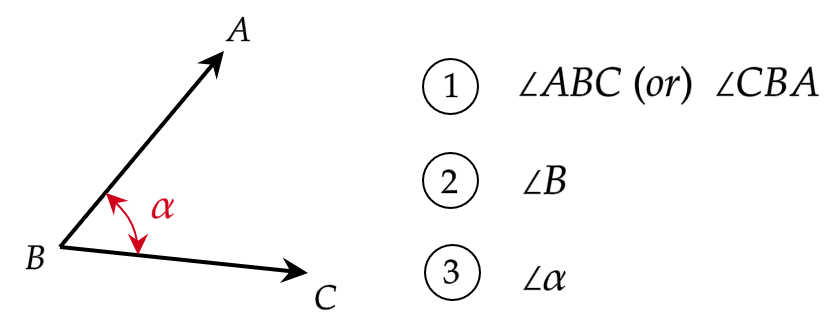
\includegraphics[scale=0.28]{pics/name_angles.png}
    \end{figure}
\end{frame}
%%%%%%%%%%%%%%%%%%%%%%%%%%%%%%%%%%%%%%%
%        SLIDE 
%%%%%%%%%%%%%%%%%%%%%%%%%%%%%%%%%%%%%%%
\section{Measure of Angles}
\begin{frame}[t]{Measure of Angles}
    \begin{itemize}
        \item The amount of rotation from one side to other is the measure of an angle.
        \item Angles can be measure in degrees, radians, or gradients.
        \item A protractor is used to measure angles.
        \item Let's discuss degrees and radians (most common ones).
    \end{itemize}
    %
    \begin{figure}[H]
        \centering
        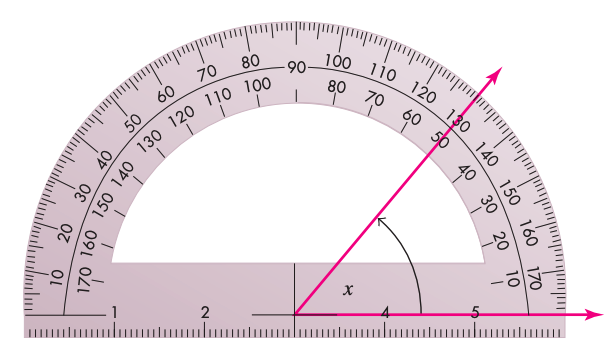
\includegraphics[scale=0.3]{pics/protractor.png}
        \caption*{Can you tell the measure of angle $\angle x$?}
    \end{figure}
\end{frame}
%%%%%%%%%%%%%%%%%%%%%%%%%%%%%%%%%%%%%%%
%        SLIDE 
%%%%%%%%%%%%%%%%%%%%%%%%%%%%%%%%%%%%%%%
\subsection{Degrees vs Radians}
\begin{frame}[t]{Degrees vs Radians}
    \begin{columns}[t]
    %1st
    \column{0.45\textwidth}
    \textbf{Degrees}
        \begin{itemize}
            \item We use $^\circ$ to denote an angle in degree.
            \item Here, full rotation is $360^\circ$.
            \item So if we divide a circle into equally $360$ parts, each part is $1^\circ$.
        \end{itemize}
        %
        \begin{figure}[H]
            \centering
            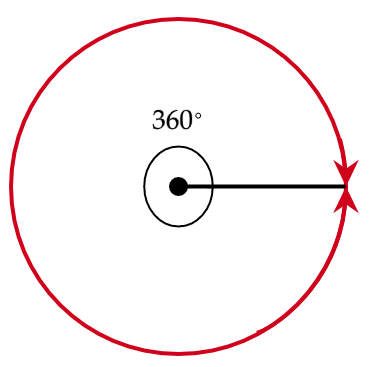
\includegraphics[width=0.45\textwidth]{pics/degrees.png}
        \end{figure}
    %2nd
    \column{0.45\textwidth}
    \textbf{Radians}
        \begin{itemize}
            \item It is a pure measure based on the Radius of the circle.
            \item If the arc between two points is equal to radius (R), corresponding angle is 1 radian. So, full rotation is $2\pi$.
        \end{itemize}
        %
        \vspace{0.5em}
        \begin{figure}[H]
            \centering
            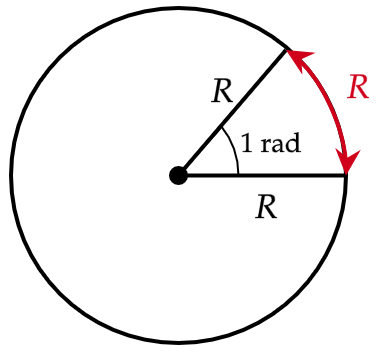
\includegraphics[width=0.45\textwidth]{pics/radians.png}
        \end{figure}
    \end{columns}
\end{frame}
%%%%%%%%%%%%%%%%%%%%%%%%%%%%%%%%%%%%%%%
%        SLIDE 
%%%%%%%%%%%%%%%%%%%%%%%%%%%%%%%%%%%%%%%
\subsection{Common Angles}
\begin{frame}{Common Angles}
    \begin{figure}[H]
        \centering
        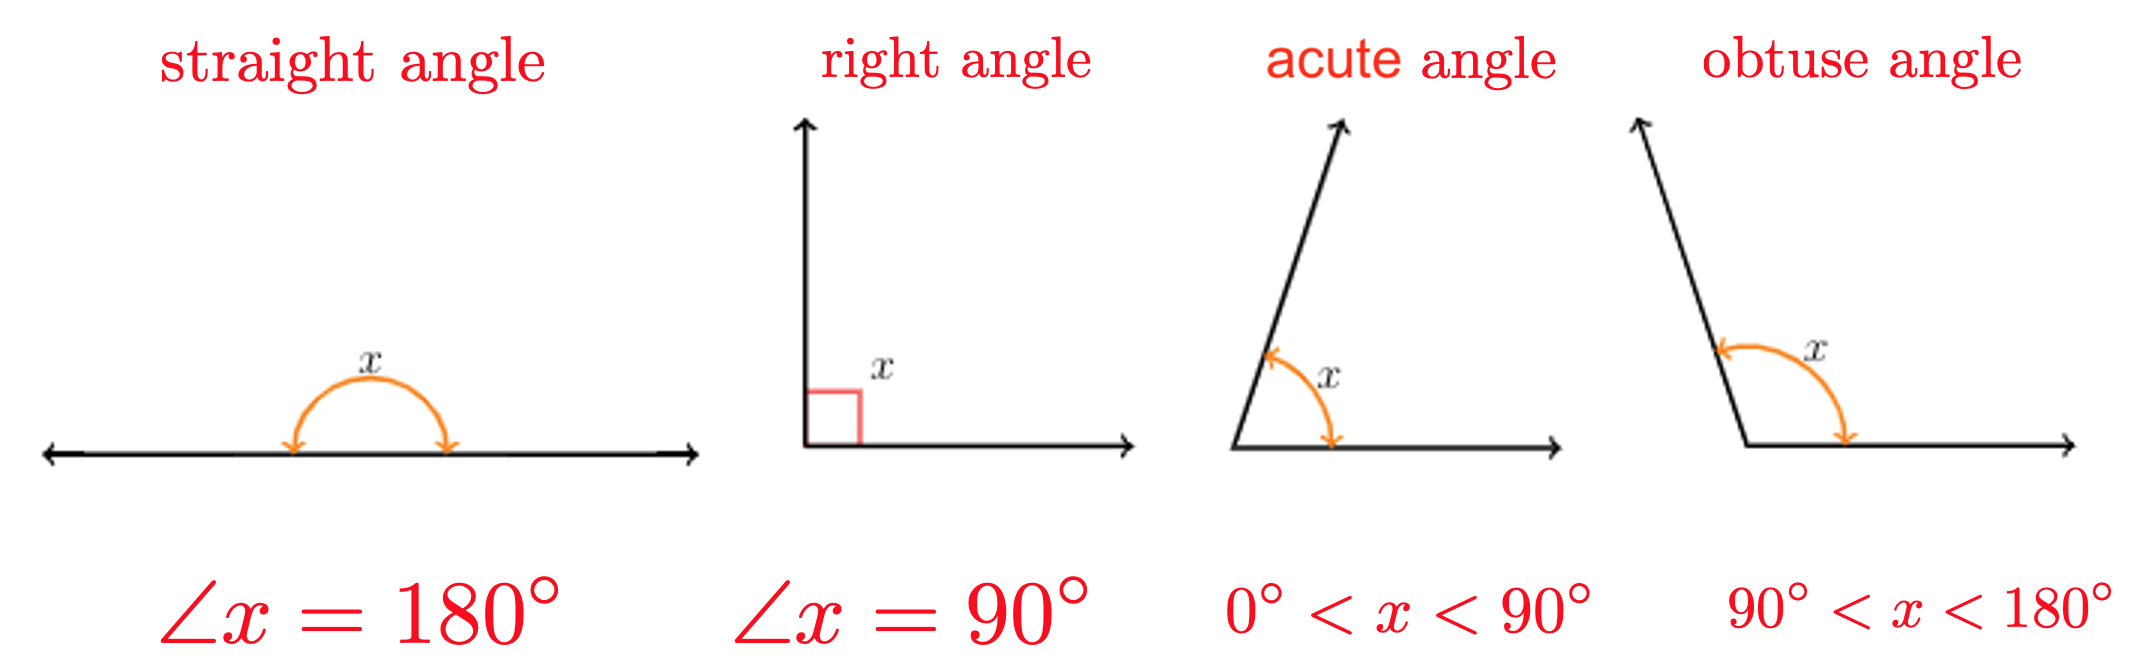
\includegraphics[scale=0.4]{pics/common_angles.png}
    \end{figure}
\end{frame}
%%%%%%%%%%%%%%%%%%%%%%%%%%%%%%%%%%%%%%%
%        SLIDE 
%%%%%%%%%%%%%%%%%%%%%%%%%%%%%%%%%%%%%%%
\addtocontents{toc}{\newpage}
%%%%%%%%%%%%%%%%%%%%%%%%%%%%%%%%%%%%%%%
\section{Important Angles}
\subsection{Adjacent Angles}
\begin{frame}{Adjacent Angles}
    \begin{block}{Definition}
        Angles that have \textbf{a common vertex and a common side but do not overlap} are called adjacent angles.
    \end{block}
    %
    \begin{figure}[H]
        \centering
        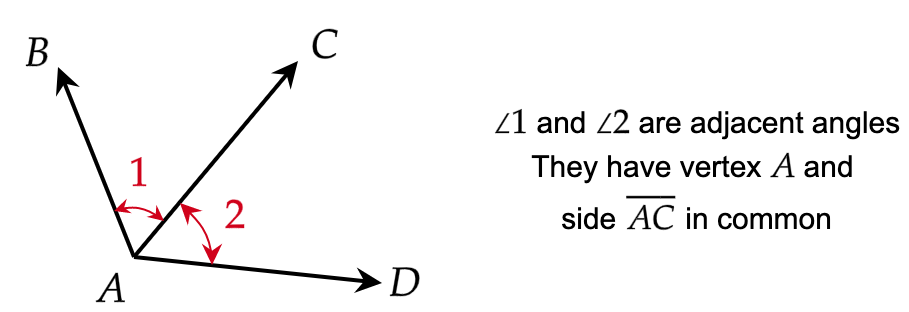
\includegraphics[scale=0.3]{pics/adjacent.png}
    \end{figure}
\end{frame}
%%%%%%%%%%%%%%%%%%%%%%%%%%%%%%%%%%%%%%%
%        SLIDE 
%%%%%%%%%%%%%%%%%%%%%%%%%%%%%%%%%%%%%%%
\subsection{Supplementary Angles}
\begin{frame}[t]{Supplementary and Complementary Angles}
    \begin{columns}
    %
    \column{0.42\textwidth}
    \begin{block}{Supplementary Angles}
        If two angles add up to $180^\circ$, then they are supplementary angles.
    \end{block}
    %
    \begin{figure}[H]
        \centering
        \usetikzlibrary{quotes,angles}
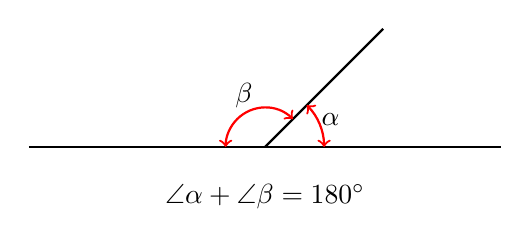
\begin{tikzpicture}[scale=1.5]
  %
  \coordinate (a) at (-2,0);
  \coordinate (o) at (0,0) node[below=1em] {$\angle \alpha + \angle \beta = 180^\circ$};
  \coordinate (c) at (1,1);
  \coordinate (d) at (2,0);
  %
  \draw[thick] (a) -- (o);
  \draw[thick] (o) -- (c);
  \draw[thick] (o) -- (d);
  %
  \draw pic["$\alpha$", thick, draw=red, <->, angle eccentricity=1.2, angle radius=0.75cm] {angle=d--o--c};
   \draw pic["$\beta$", thick, draw=red, <->, angle eccentricity=1.4, angle radius=0.5cm] {angle=c--o--a};
   
\end{tikzpicture}
    \end{figure}
    %
    \column{0.42\textwidth}
    \begin{block}{Complementary Angles}
        If two angles add up to $90^\circ$, then they are complementary angles.
    \end{block}
    %
    \begin{figure}[H]
        \centering
        \usetikzlibrary{quotes,angles}
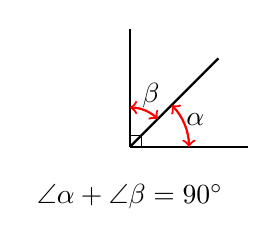
\begin{tikzpicture}[scale=1.5]
  %
  \coordinate (a) at (0,1);
  \coordinate (o) at (0,0) node[below=1em] {$\angle \alpha + \angle \beta = 90^\circ$};
  \coordinate (c) at (1,0);
  \coordinate (d) at (0.75,0.75);
  %
  \draw[thick] (a) -- (o);
  \draw[thick] (o) -- (c);
  \draw[thick] (o) -- (d);
  %
  \draw pic["$\alpha$", thick, draw=red, <->, angle eccentricity=1.2, angle radius=0.75cm] {angle=c--o--d};
   \draw pic["$\beta$", thick, draw=red, <->, angle eccentricity=1.4, angle radius=0.5cm] {angle=d--o--a};
   %
   \draw (o) -- (0,0.1) -- (0.1,0.1) -- (0.1,0);
\end{tikzpicture}
    \end{figure}
    %    
    \end{columns}
\end{frame}
%%%%%%%%%%%%%%%%%%%%%%%%%%%%%%%%%%%%%%%
%        SLIDE 
%%%%%%%%%%%%%%%%%%%%%%%%%%%%%%%%%%%%%%%
\subsection{Vertical Angles}
\begin{frame}[t]{Vertical Angles}
    \begin{block}{Definition}
        \begin{itemize}
            \item When two straight lines intersect, the non-adjacent angles
		    are called vertical angles.
		    \item Vertical angles are equal.
        \end{itemize}
    \end{block}
    %
    \begin{columns}
    \column{0.45\textwidth}
    Opposite angles are vertical angles. So,
    \begin{align*}
         \angle 1 &= \angle 3
         \\
         \angle 2 &= \angle 4
    \end{align*}
    %
    \column{0.45\textwidth}
    \begin{figure}[H]
        \centering
        \usetikzlibrary{quotes,angles}
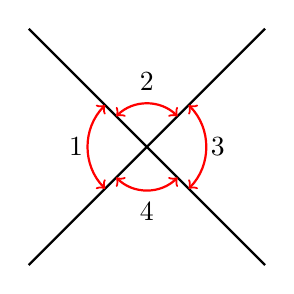
\begin{tikzpicture}[scale=1.5]
  %
  \coordinate (a) at (-1,1);
  \coordinate (o) at (0,0) ;
  \coordinate (b) at (1,-1);
  \coordinate (d) at (1,1);
  \coordinate (e) at (-1,-1);
  %
  \draw[thick] (a) -- (b);
  \draw[thick] (e) -- (d);
  %
   \draw pic["$1$", thick, draw=red, <->, angle eccentricity=1.2, angle radius=0.75cm] {angle=a--o--e};
   \draw pic["$2$", thick, draw=red, <->, angle eccentricity=1.5, angle radius=0.55cm] {angle=d--o--a};
   \draw pic["$3$", thick, draw=red, <->, angle eccentricity=1.2, angle radius=0.75cm] {angle=b--o--d};
   \draw pic["$4$", thick, draw=red, <->, angle eccentricity=1.5, angle radius=0.55cm] {angle=e--o--b};
   %
\end{tikzpicture}
    \end{figure}  
          %
    \end{columns}
\end{frame}
%%%%%%%%%%%%%%%%%%%%%%%%%%%%%%%%%%%%%%%
%        SLIDE 
%%%%%%%%%%%%%%%%%%%%%%%%%%%%%%%%%%%%%%%
\begin{frame}[t]{Example (Find Missing Angles)}
    \begin{example}
    \begin{columns}[t]
    \column{0.7\textwidth}
     \small{$\angle CBA$ is equal to $20^\circ$.}
     \begin{enumerate}[(a)]
         \item \small{If $\angle DBC$ and $\angle CBA$ are complementary angles, find $\angle DBC$.}
         \item \small{If $\angle CBA$ and $\angle CBE$ are supplementary angles, find $\angle DBE$.}
     \end{enumerate}
     %
     \column{0.3\textwidth}
     \begin{figure}[H]
         \centering
         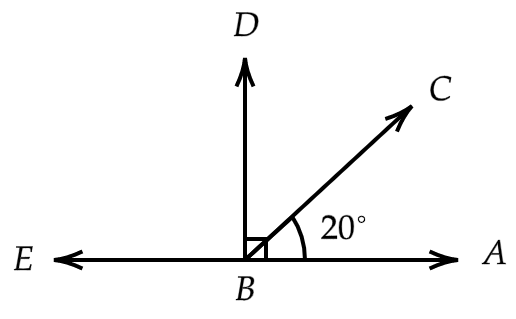
\includegraphics[scale=0.25]{pics/example_1.png}
     \end{figure}
     \end{columns}
    \end{example}
\end{frame}
%%%%%%%%%%%%%%%%%%%%%%%%%%%%%%%%%%%%%%%
%        SLIDE 
%%%%%%%%%%%%%%%%%%%%%%%%%%%%%%%%%%%%%%%
\section{Transversal Line}
\begin{frame}{Transversal Line}
    \begin{block}{Definition}
        \begin{itemize}
            \item A transversal line is a line that intersects two different lines at different points.
            \item A transveral line forms eight angles.
        \end{itemize}
    \end{block}
    %
    \begin{figure}[H]
        \centering
        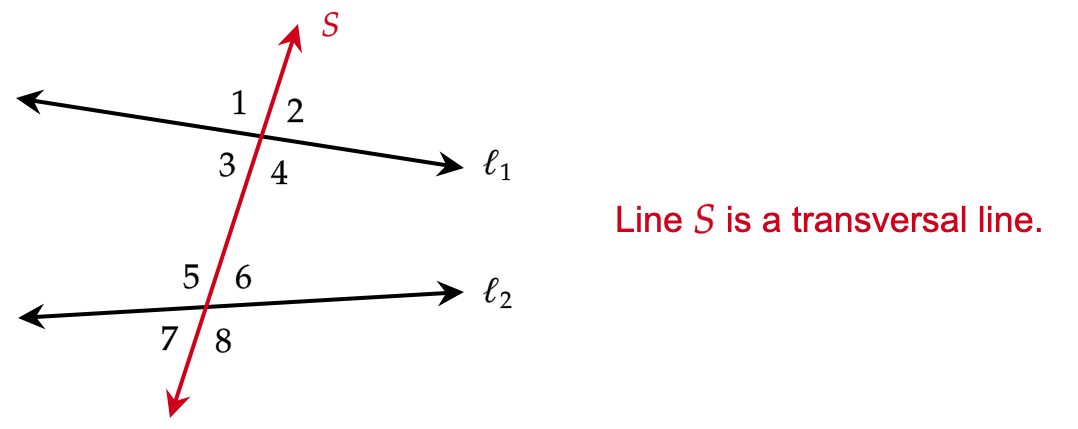
\includegraphics[scale=0.3]{pics/transversal_line.png}
    \end{figure}
\end{frame}
%%%%%%%%%%%%%%%%%%%%%%%%%%%%%%%%%%%%%%%
%        SLIDE 
%%%%%%%%%%%%%%%%%%%%%%%%%%%%%%%%%%%%%%%
\subsection{Interior and Exterior Angles}
\begin{frame}[t]{Interior and Exterior Angles}
    \begin{columns}
    \column{0.45\textwidth}
    %
    \textbf{Interior Angles}
    \begin{itemize}
        \item Angles that are form inside $\ell_1$ and $\ell_2$ are called \textit{interior angles}.
    \end{itemize}
    %
    %
    \begin{figure}[H]
        \centering
        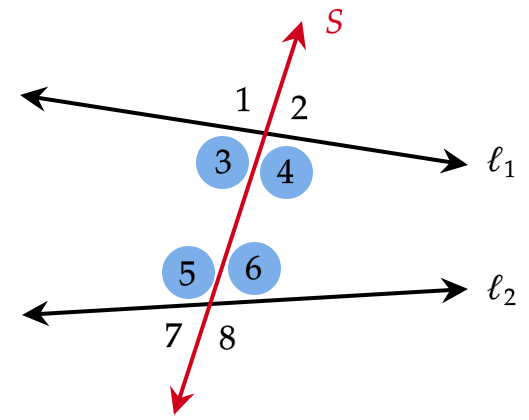
\includegraphics[scale=0.3]{pics/interior_angles.png}
    \end{figure}    
    \column{0.45\textwidth}
    %
    \textbf{Exterior Angles}
    \begin{itemize}
        \item Angles that are form outside $\ell_1$ and $\ell_2$ are called \textit{exterior angles}.
    \end{itemize}
    %    
    \begin{figure}[H]
        \centering
        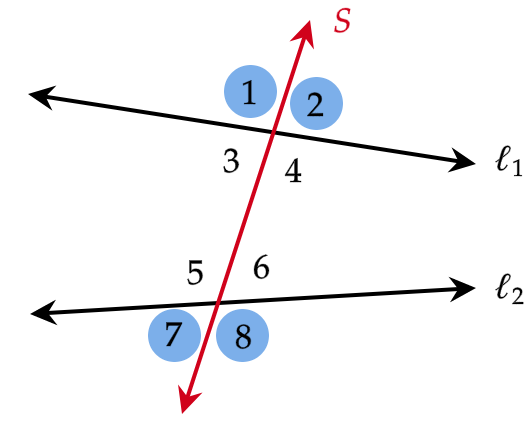
\includegraphics[scale=0.3]{pics/exterior_angles.png}
    \end{figure} 
    \end{columns}
\end{frame}
%%%%%%%%%%%%%%%%%%%%%%%%%%%%%%%%%%%%%%%
%        SLIDE 
%%%%%%%%%%%%%%%%%%%%%%%%%%%%%%%%%%%%%%%
\subsection{Corresponding Angles}
\begin{frame}{Corresponding Angles}
    \begin{itemize}
        \item one exterior angle and one interior angle on the same side of transversal line are called \textit{corresponding angles} for these lines.
    \end{itemize}
    %
    \begin{figure}[H]
        \centering
        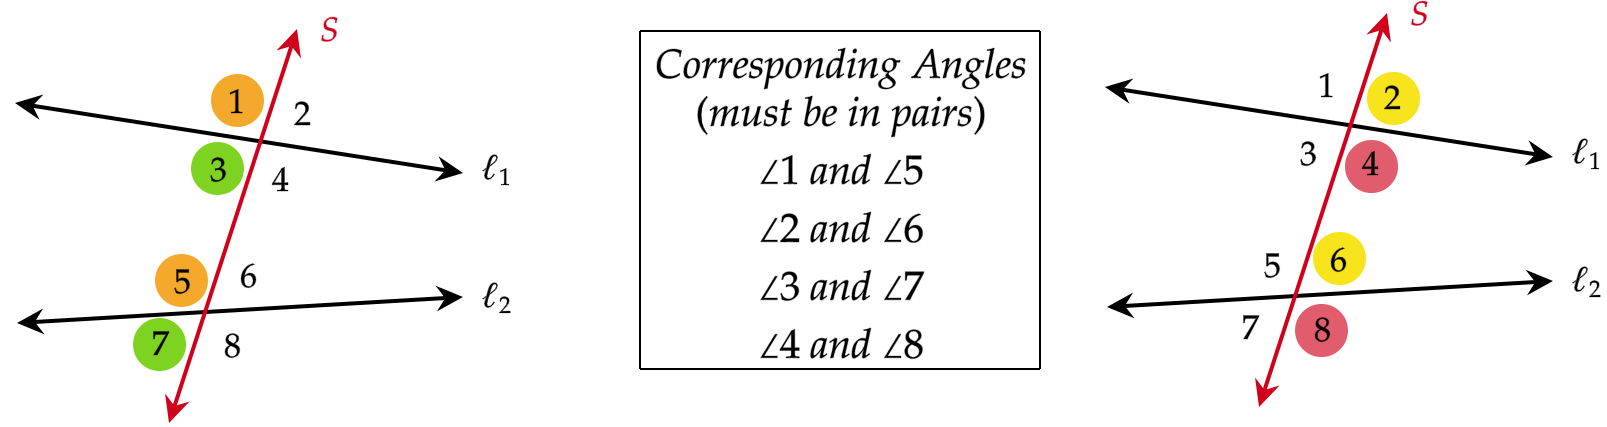
\includegraphics[scale=0.25]{pics/corresponding.png}
    \end{figure}
\end{frame}
%%%%%%%%%%%%%%%%%%%%%%%%%%%%%%%%%%%%%%%
%        SLIDE 
%%%%%%%%%%%%%%%%%%%%%%%%%%%%%%%%%%%%%%%
\subsection{Alternate Interior Angles}
\begin{frame}{Alternate Interior Angles}
    \begin{itemize}
        \item Two interior angles that have different vertices and lie on opposite sides of the transversal are \textit{alternate interior angles}.
    \end{itemize}
    %
    \begin{figure}[H]
        \centering
        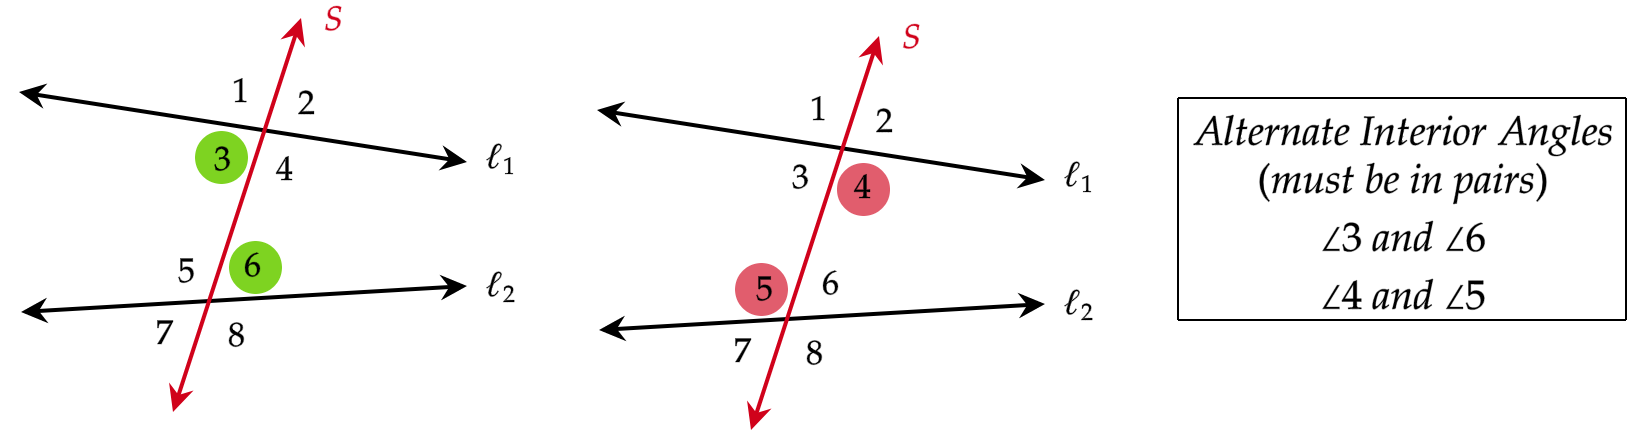
\includegraphics[scale=0.25]{pics/alternate_interior_angles.png}
    \end{figure}
\end{frame}
%%%%%%%%%%%%%%%%%%%%%%%%%%%%%%%%%%%%%%%
%        SLIDE 
%%%%%%%%%%%%%%%%%%%%%%%%%%%%%%%%%%%%%%%
\subsection{Alternate Exterior Angles}
\begin{frame}{Alternate Exterior Angles}
    \begin{itemize}
        \item Two exterior angles that have different vertices and lie on opposite sides of the transversal are \textit{alternate exterior angles}.
    \end{itemize}
    %
    \begin{figure}[H]
        \centering
        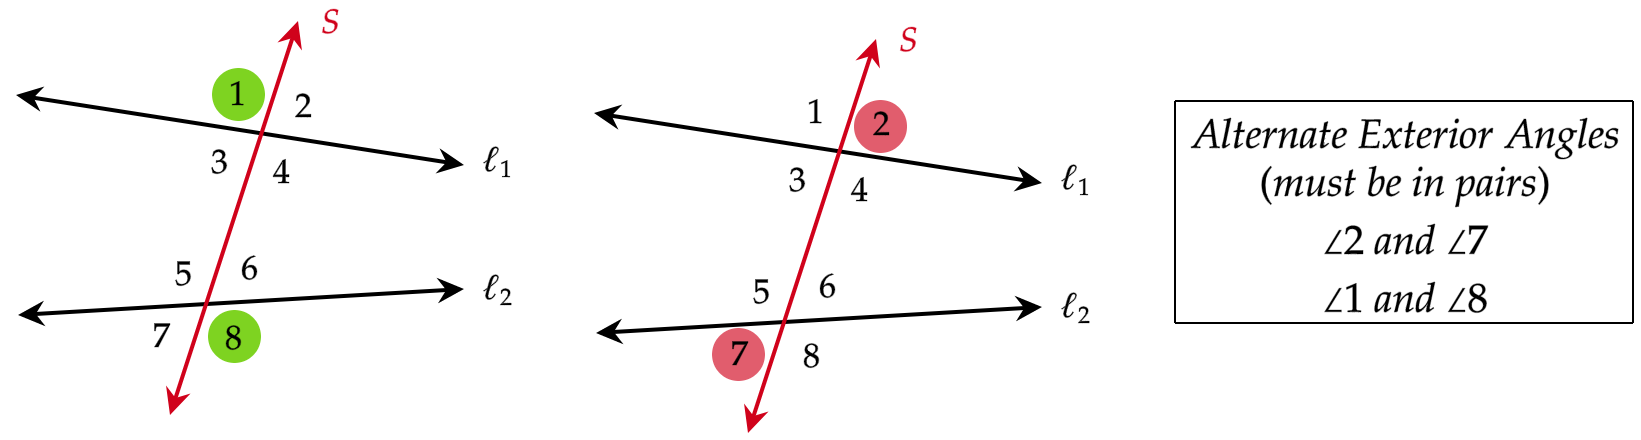
\includegraphics[scale=0.25]{pics/alternate_exterior_angles.png}
    \end{figure}
\end{frame}
%%%%%%%%%%%%%%%%%%%%%%%%%%%%%%%%%%%%%%%
%        SLIDE 
%%%%%%%%%%%%%%%%%%%%%%%%%%%%%%%%%%%%%%%
\section{Parallel lines and a Transversal Line}
\begin{frame}{Parallel lines and a Transversal Line}
    \begin{itemize}
        \item If a transversal line intersects two parallel lines, then
    \end{itemize}
    \begin{figure}[H]
        \centering
        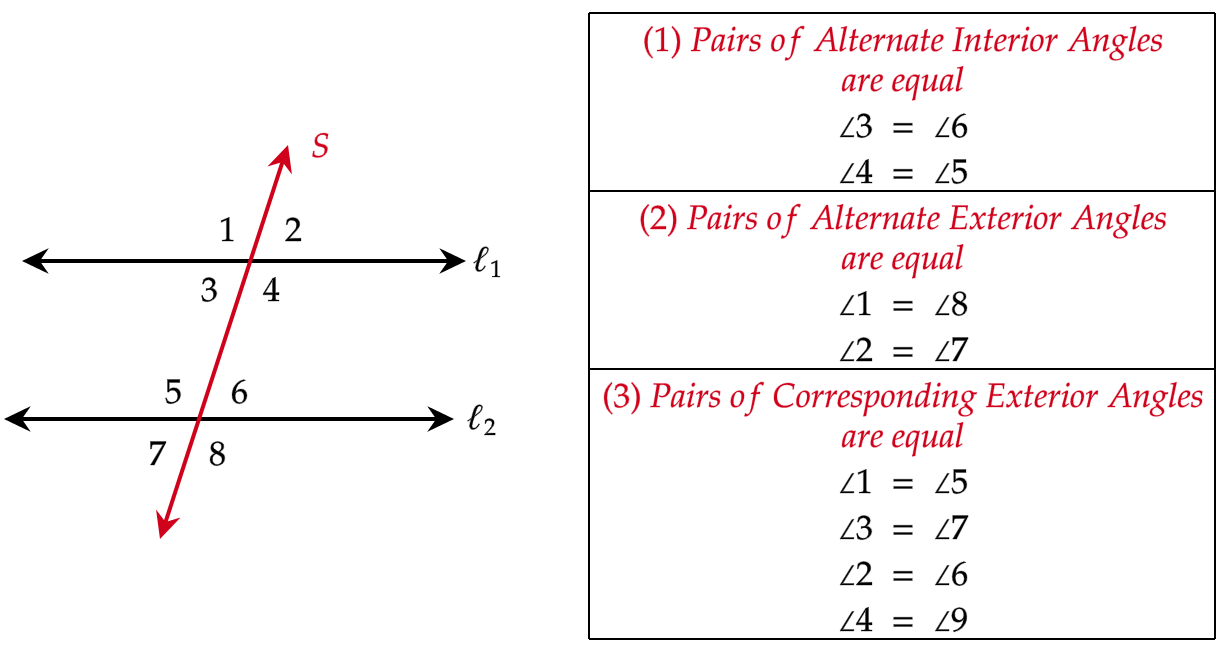
\includegraphics[scale=0.28]{pics/parallel_transversal.png}
    \end{figure}
\end{frame}
%%%%%%%%%%%%%%%%%%%%%%%%%%%%%%%%%%%%%%%
%        SLIDE 
%%%%%%%%%%%%%%%%%%%%%%%%%%%%%%%%%%%%%%%
\subsection{Summary}
\begin{frame}{Summary}
    \begin{figure}[H]
        \centering
        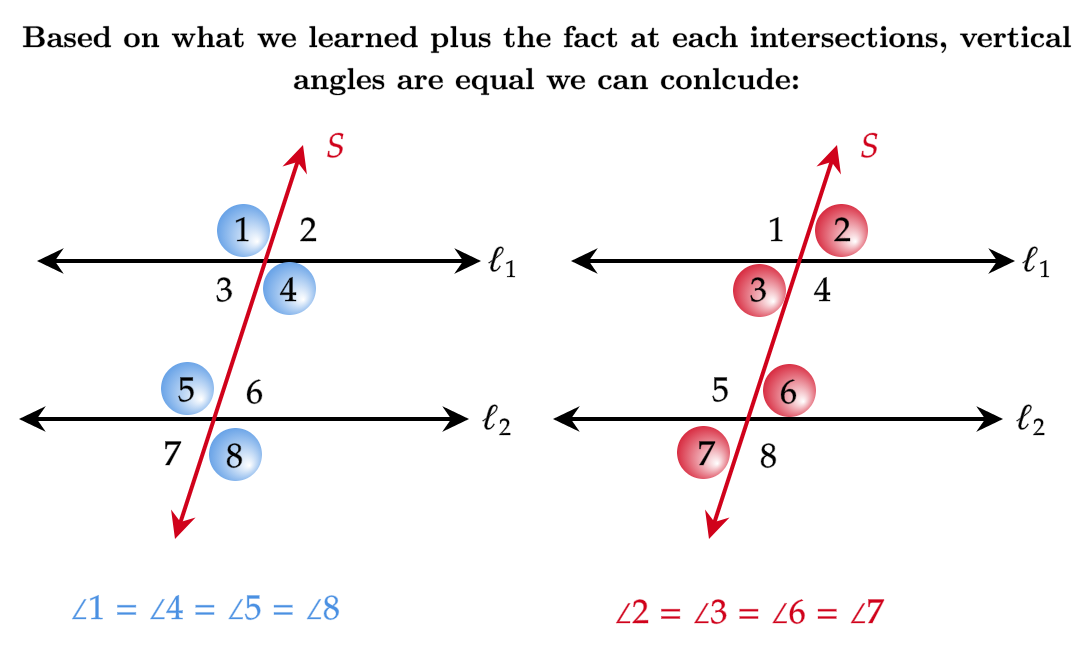
\includegraphics[scale=0.3]{pics/summaray_parallel.png}
    \end{figure}
\end{frame}
%%%%%%%%%%%%%%%%%%%%%%%%%%%%%%%%%%%%%%%
%        SLIDE 
%%%%%%%%%%%%%%%%%%%%%%%%%%%%%%%%%%%%%%%
\begin{frame}[t]{Example (Parallel Lines)}
    \begin{example}
        \begin{columns}[t]
        \column{0.45\textwidth}
        In figure below, line $\ell$ is parallel to line $m$ and $\angle 2 =117^\circ$. Determine all remaining angles.
        %
        \column{0.45\textwidth}
        \begin{figure}[H]
            \centering
            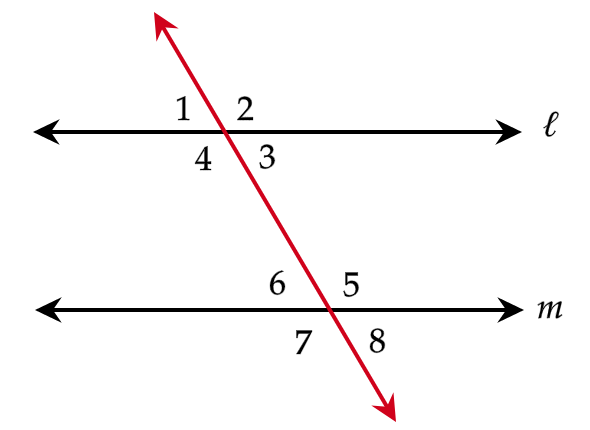
\includegraphics[scale=0.2]{pics/parallel_example.png}
        \end{figure}
        \end{columns}
    \end{example}
\end{frame}
% PART 2 (SECTION 8.2)
\part{Section 8.2}
%%%%%%%%%%%%%%%%%%%%%%%%%%%%%%%%%%%%%%%
\begin{transitionframe}
    \begin{center}
    { 
        \Huge \textcolor{white}{\textbf{Polygons}}
        \\[-1em]
        \noindent\textcolor{white}{\rule{12cm}{0.4pt}}
        
        %\large \textcolor{white}{Section 8.2}
    }
    \end{center}
\end{transitionframe}
%%%%%%%%%%%%%%%%%%%%%%%%%%%%%%%%%%%%%%%
%        SLIDE 
%%%%%%%%%%%%%%%%%%%%%%%%%%%%%%%%%%%%%%%
\begin{frame}{Outline}
    \begin{columns}[t]
        \begin{column}{.5\textwidth}
            \tableofcontents[part=2, sections={1-3}]
        \end{column}
        \begin{column}{.5\textwidth}
            \tableofcontents[part=2, sections={4-5}]
        \end{column}
    \end{columns}
\end{frame}
%%%%%%%%%%%%%%%%%%%%%%%%%%%%%%%%%%%%%%%
%        SLIDE 
%%%%%%%%%%%%%%%%%%%%%%%%%%%%%%%%%%%%%%%
\section{Polygons}
\subsection{What is a Polygon?}
\begin{frame}[t]{What is a Polygon?}
    \begin{itemize}
        \item Polygon is another word derived from Greek meaning ``many angles''.
    \end{itemize}
    %
    \begin{block}{Definition}
        A shape that meets the following conditions are called polygon:
        \begin{itemize}
            \item closed shape
            \item made of only straight lines
            \item 2-Dimensional shape
        \end{itemize}
    \end{block}
    %
    \begin{figure}[H]
        \centering
        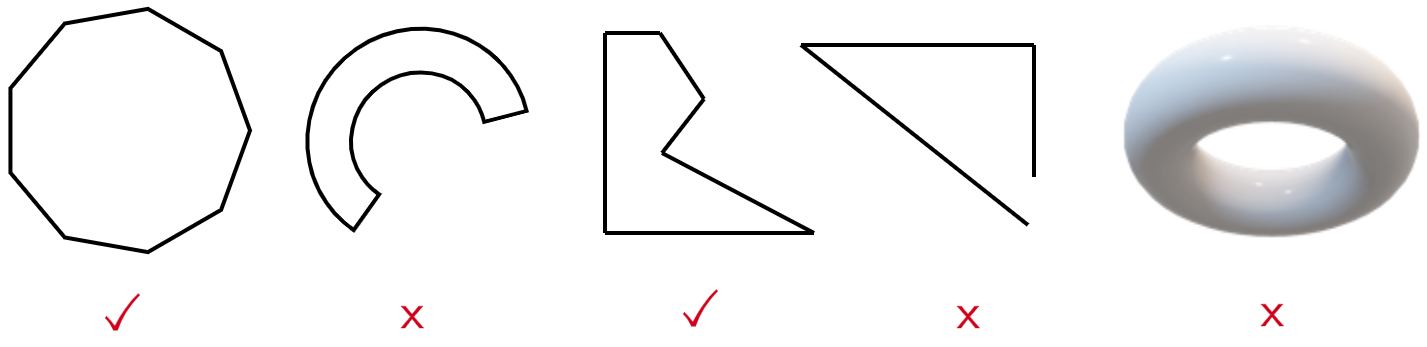
\includegraphics[scale=0.2]{pics/polygons.png}
    \end{figure}
\end{frame}
%%%%%%%%%%%%%%%%%%%%%%%%%%%%%%%%%%%%%%%
%        SLIDE 
%%%%%%%%%%%%%%%%%%%%%%%%%%%%%%%%%%%%%%%
\subsection{Sides and Vertices}
\begin{frame}{Sides and Vertices}
    \begin{itemize}
        \item Each straight-line segments are called \textit{sides}.
        \item A point where two sides meet is called a \textit{vertex (plural Vertices)}.
    \end{itemize}
    %
    \begin{figure}[H]
        \centering
        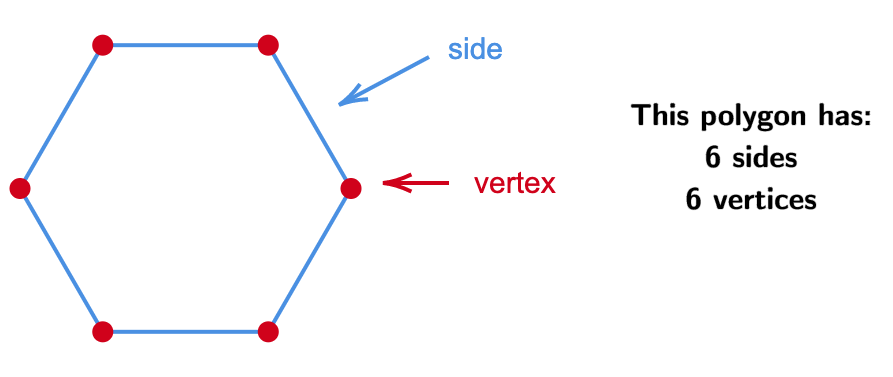
\includegraphics[scale=0.35]{pics/sides_vertices.png}
    \end{figure}
\end{frame}
%%%%%%%%%%%%%%%%%%%%%%%%%%%%%%%%%%%%%%%
%        SLIDE 
%%%%%%%%%%%%%%%%%%%%%%%%%%%%%%%%%%%%%%%
\subsection{Interior and Exterior Angles}
\begin{frame}[t]{Interior and Exterior Angles}
    \begin{columns}[t]
    %
    \column{0.45\textwidth}
    \textbf{Interior Angles}
    \begin{itemize}
        \item An angle formed by two adjacent sides inside the polygon.
    \end{itemize}
    %
    \column{0.45\textwidth}
    \textbf{Exterior Angles}
    \begin{itemize}
        \item An angle at a vertex of the polygon, outside the polygon, formed by one side and the extension of an adjacent side.
    \end{itemize}
    \end{columns}
    %
    \begin{figure}[H]
        \centering
        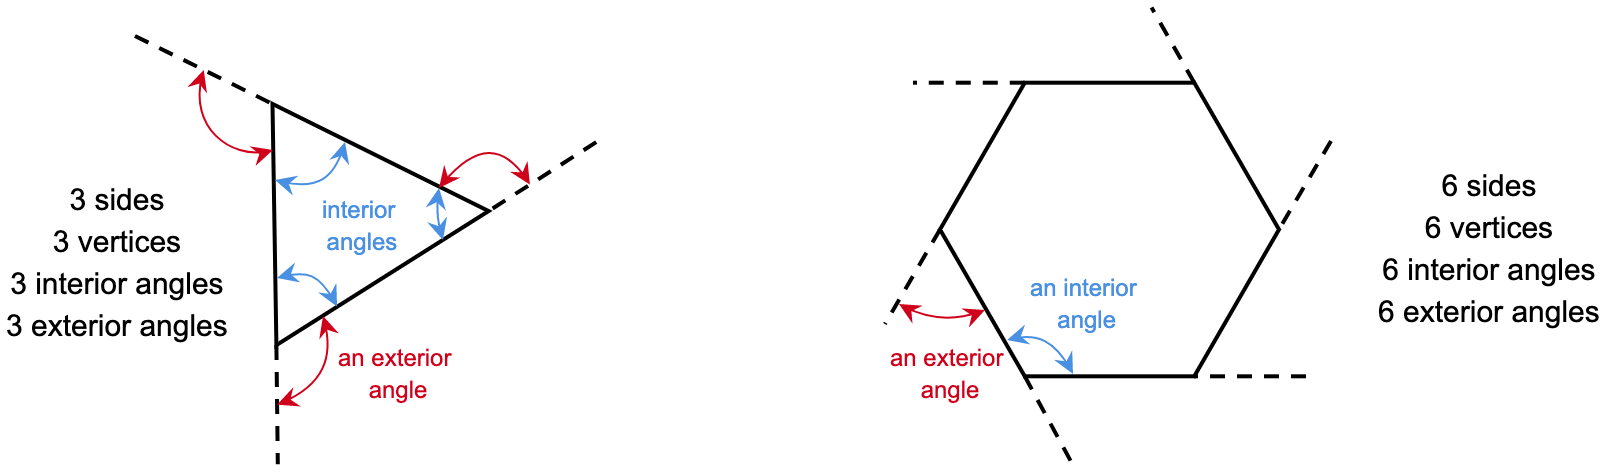
\includegraphics[scale=0.26]{pics/interior_exterior_polygons.png}
    \end{figure}
\end{frame}
%%%%%%%%%%%%%%%%%%%%%%%%%%%%%%%%%%%%%%%
%        SLIDE 
%%%%%%%%%%%%%%%%%%%%%%%%%%%%%%%%%%%%%%%
\subsection{Name of Some Polygons}
\begin{frame}{Name of Some Polygons}
    \begin{itemize}
        \item Polygons are named according to their number of sides.
    \end{itemize}
    %
    \begin{table}[H]
    \centering
    \begin{tabular}{c c || c  c}
        \toprule
        Number of sides & Name &  Number of sides  & Name\\
        \hline
        3 & Triangle        &   8       & Octagon
        \\ 
        4 & Quadrilateral   &   9       & Nanogon
        \\ 
        5 & Pentagon        &   10      & Decagon
        \\  
        6 & Hexagon         &   12      & Dodecagon
        \\
        7 & Heptagon        &   20      & Icosagan
        \\ \bottomrule
    \end{tabular}
    \label{tab:polygons_names}
\end{table}
\end{frame}
%%%%%%%%%%%%%%%%%%%%%%%%%%%%%%%%%%%%%%%
%        SLIDE 
%%%%%%%%%%%%%%%%%%%%%%%%%%%%%%%%%%%%%%%
\subsection{Regular Polygons}
\begin{frame}[t]{Regular Polygons}
    \begin{itemize}
        \item All sides are equal.
        \item All interior angles are equal.
        \item All exterior angles are equal.
    \end{itemize}
    %
    \begin{figure}[H]
        \centering
        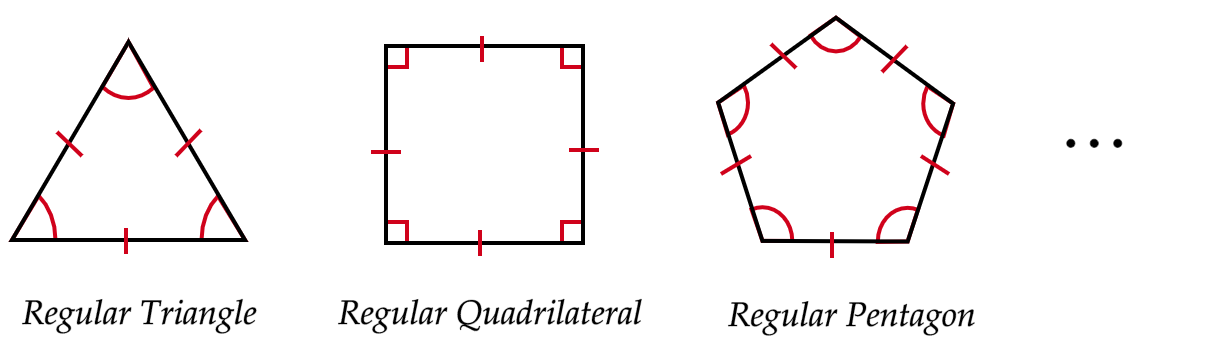
\includegraphics[scale=0.3]{pics/regular_polygon.png}
    \end{figure}
\end{frame}
%%%%%%%%%%%%%%%%%%%%%%%%%%%%%%%%%%%%%%%
%        SLIDE 
%%%%%%%%%%%%%%%%%%%%%%%%%%%%%%%%%%%%%%%
\section{More on Interior Angles}
\subsection{Sum of Interior Angles}
\begin{frame}[t]{Sum of Interior Angles}
    \begin{itemize}
        \item It can be proven that sum of interior angles in a triangle is equal to $180^\circ$.
        \item Using this fact, we can find sum of interior angles in other polygons.
    \end{itemize}
    %
    \begin{figure}[H]
        \centering
        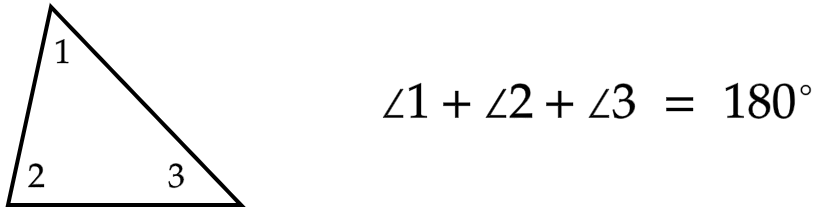
\includegraphics[scale=0.3]{pics/sum_angles_triangle.png}
    \end{figure}
    %
    \begin{itemize}
        \item To find the sum of interior angles in other polygons, we must ask ourselves how many triangles we can create inside a polygons?
        \item Is there any relationship between number of triangles created insides a polygon and number of sides?
    \end{itemize}
\end{frame}
%%%%%%%%%%%%%%%%%%%%%%%%%%%%%%%%%%%%%%%
%        SLIDE 
%%%%%%%%%%%%%%%%%%%%%%%%%%%%%%%%%%%%%%%
\begin{frame}{}
    \begin{figure}[H]
        \centering
        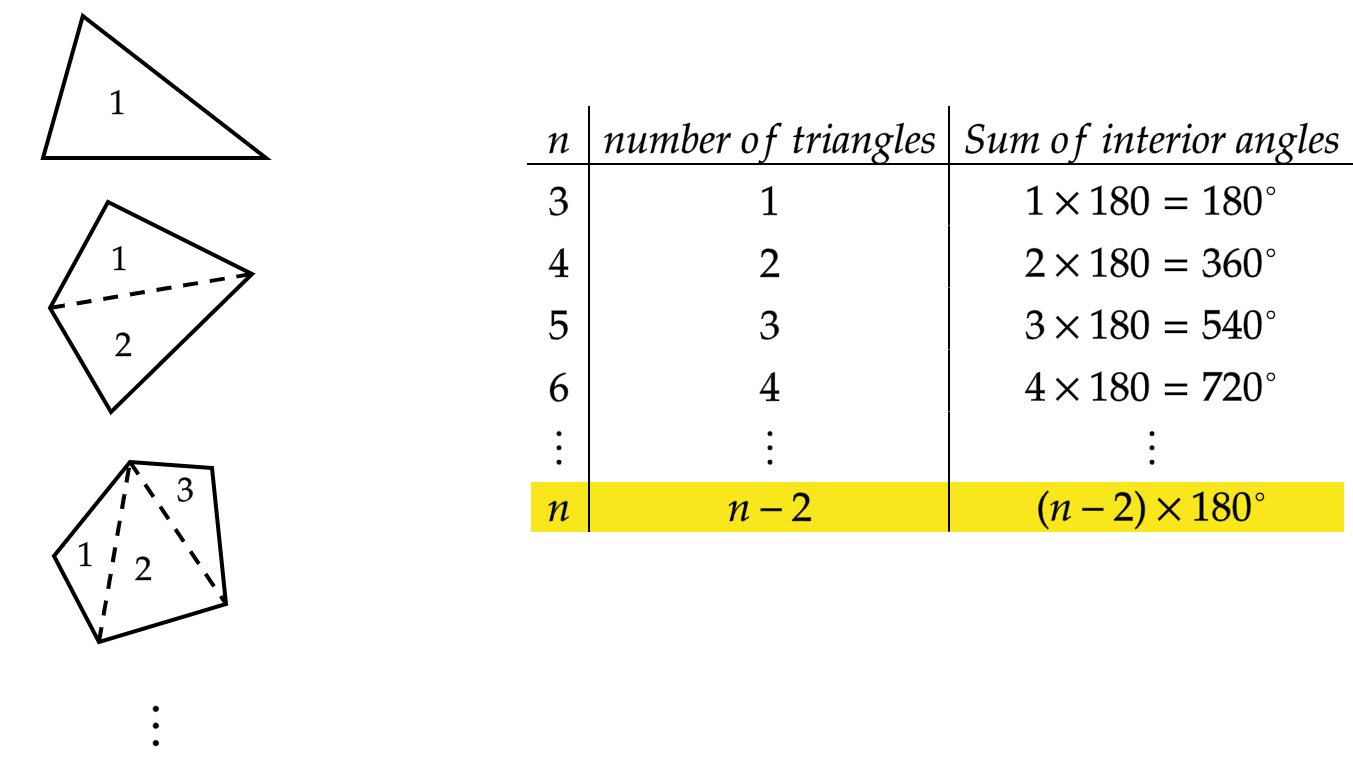
\includegraphics[scale=0.3]{pics/general_sum_of_interior.png}
    \end{figure}
\end{frame}
%%%%%%%%%%%%%%%%%%%%%%%%%%%%%%%%%%%%%%%
%        SLIDE 
%%%%%%%%%%%%%%%%%%%%%%%%%%%%%%%%%%%%%%%
\begin{frame}[t]{Example (Sum of Interior Angles)}
    \begin{example}
        \begin{itemize}
            \item Find sum of interior angles in
            \begin{enumerate}[(a)]
                \item Decagon
                \item Octagon
                \item 30-gon
            \end{enumerate}
        \end{itemize}
    \end{example}
\end{frame}
%%%%%%%%%%%%%%%%%%%%%%%%%%%%%%%%%%%%%%%
%        SLIDE 
%%%%%%%%%%%%%%%%%%%%%%%%%%%%%%%%%%%%%%%
\subsection{An Interior Angle of a Regular Polygon}
\begin{frame}[t]{An Interior Angle of a Regular Polygon}
    \begin{columns}
    \column{0.5\textwidth}
    \begin{itemize}
        \item Consider a regular polygon.
        \item In a regular polygon, all interior angles are equal. 
        \item Thus, we can easily find the measure of an interior angle by dividing the sum of interior angles by number of sides.
    \end{itemize}
    %
    \column{0.45\textwidth}
    \begin{figure}[H]
        \centering
        
\includegraphics[scale=0.05]{pics/bam.jpg}
    \end{figure}
    \end{columns}
    %
    \begin{block}{Measure of an interior angle in a regular polygon}
    An interior angle of a \textbf{regular polygon} can be find as follow:
    \[
        \text{an interior angle of a regular polygon} = \frac{\text{Sum of interior angles}}{\text{Number of sides}}   
        \label{for::interior_angle}    
    \]
    \end{block}
    %
\end{frame}
%%%%%%%%%%%%%%%%%%%%%%%%%%%%%%%%%%%%%%%%%%%%%%%%
%        SLIDE 
%%%%%%%%%%%%%%%%%%%%%%%%%%%%%%%%%%%%%%%%%%%%%%%%
\begin{frame}[t]{Example (Measure of an Interior Angle)}
    \begin{example}
        Find the measure of an interior angle in a regular octagon.
    \end{example}
\end{frame}
%%%%%%%%%%%%%%%%%%%%%%%%%%%%%%%%%%%%%%%%%%%%%%%%
%        SLIDE 
%%%%%%%%%%%%%%%%%%%%%%%%%%%%%%%%%%%%%%%%%%%%%%%%
\section{More on Exterior Angles}
\subsection{Sum of Exterior Angles}
\begin{frame}[t]{Sum of Exterior Angles}
    \begin{itemize}
        \item It can be proven that sum of exterior angles in any polygon (regular or irregular) is always equal to $360^\circ$.
    \end{itemize}
    %
\begin{figure}[H]
    \centering
    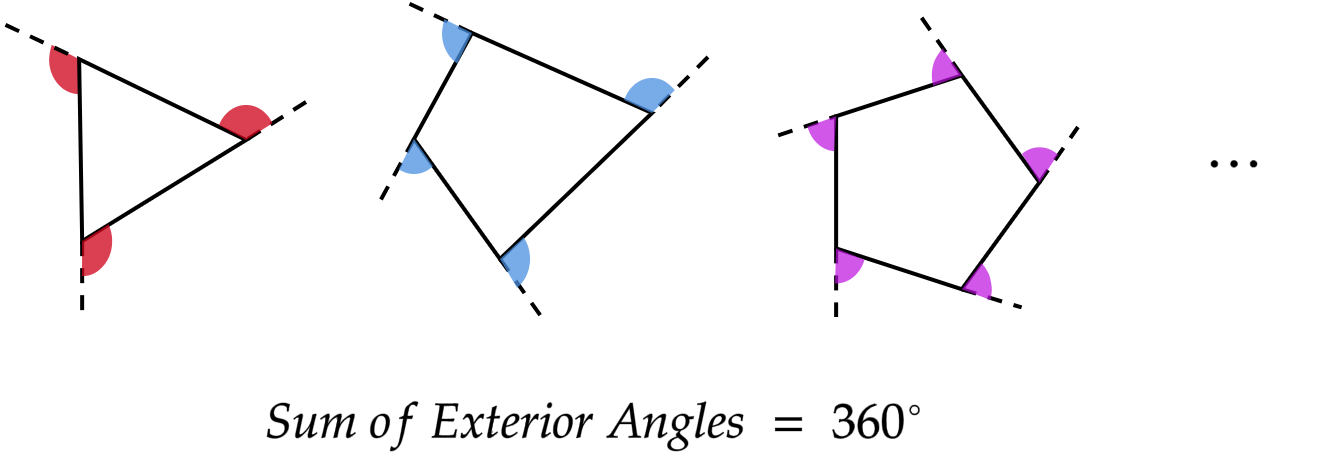
\includegraphics[scale=0.3]{pics/sum_exterior_angles.png}
\end{figure}
\end{frame}
%%%%%%%%%%%%%%%%%%%%%%%%%%%%%%%%%%%%%%%%%%%%%%%%
%        SLIDE 
%%%%%%%%%%%%%%%%%%%%%%%%%%%%%%%%%%%%%%%%%%%%%%%%
\subsection{An Exterior Angle of a Regular Polygon}
\begin{frame}[t]{An Exterior Angle of a Regular Polygon}
    %
    \begin{itemize}
        \item In a regular polygon, all exterior angles are equal.
        \item We could measure an exterior angle of a regular polygon by dividing the sum of exterior angles (which is $360^\circ$) by number of sides.
    \end{itemize}
    %
    \begin{block}{Measure of an exterior angle in a regular polygon}
    An exterior angle of a \textbf{regular polygon} can be find as follow:
    \[
        \text{an exterior angle of a regular polygon} = \frac{360^\circ}{\text{Number of sides}}   
        \label{for::exterior_angle}    
    \]
    \end{block}    
\end{frame}
%%%%%%%%%%%%%%%%%%%%%%%%%%%%%%%%%%%%%%%%%%%%%%%%
%        SLIDE 
%%%%%%%%%%%%%%%%%%%%%%%%%%%%%%%%%%%%%%%%%%%%%%%%
\begin{frame}[t]{Example (Measure of an Exterior Angle)}
    \begin{example}
        \begin{itemize}
            \item Find an exterior angle of the following regular polygons:
            \begin{enumerate}
                \item A regular hexagon
                \item A regular octagon
                \item A 14-gon
            \end{enumerate}
        \end{itemize}
    %
    \end{example}
\end{frame}
%%%%%%%%%%%%%%%%%%%%%%%%%%%%%%%%%%%%%%%
%%%%%%%%%%%%%%%%%%%%%%%%%%%%%%%%%%%%%%%%%%%%%%%%
%        SLIDE 
%%%%%%%%%%%%%%%%%%%%%%%%%%%%%%%%%%%%%%%%%%%%%%%%
\section{Triangles}
\begin{frame}{Triangles}
    \begin{itemize}
        \item There are 6 types of triangles. 
    \end{itemize}
    %
    \begin{figure}[H]
        \centering
        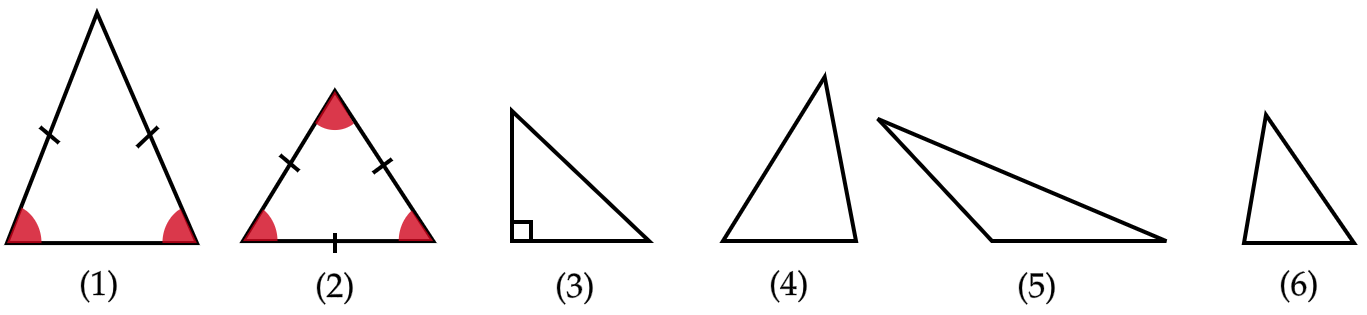
\includegraphics[scale=0.3]{pics/types_of_triangles.png}
    \end{figure}
\end{frame}
%%%%%%%%%%%%%%%%%%%%%%%%%%%%%%%%%%%%%%%%%%%%%%%%
%        SLIDE 
%%%%%%%%%%%%%%%%%%%%%%%%%%%%%%%%%%%%%%%%%%%%%%%%
\subsection{Isosceles Triangle}
\begin{frame}{Isosceles Triangle}
    \begin{itemize}
        \item Isosceles means ``same legs'' in Greek.
        \item Two sides are equal.
        \item The angles opposite the equal sides are also equal.
    \end{itemize}
    %
    \begin{columns}
    \column{0.45\textwidth}
        \begin{figure}[H]
        \centering
            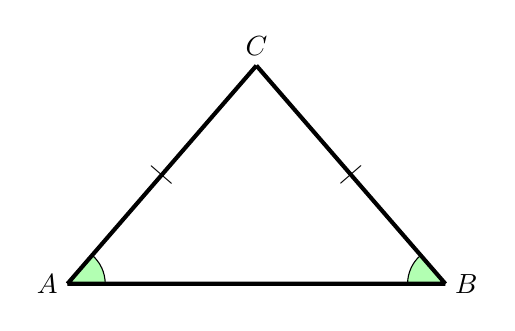
\begin{tikzpicture}[scale=0.8]
            \coordinate[label=left:$A$]  (A) at (-1,0);
            \coordinate[label=right:$B$] (B) at (5,0);
            \coordinate[label=above:$C$] (C) at (2,3.464);
    
            % angle CAB
            \begin{scope}[shift={(-1cm,0cm)}]
                \draw[fill=green!30] (0,0) -- (0:0.6cm) arc (0:50:0.6cm);
            \end{scope}
            % angle CBA
            \begin{scope}[shift={(5cm,0cm)}]
                \draw[fill=green!30] (0,0) -- (-180:0.6cm) arc (180:130:0.6cm);
            \end{scope}
            % triangle
            \draw [line width=1.5pt] (A) --  (B)
                                     (A) -- node[sloped] {$|$} (C)
                                     (B) -- node[sloped] {$|$} (C);
          \end{tikzpicture}
        \label{fig:isosceles_triangle}
    \end{figure}
    %
    \column{0.45\textwidth}
        \begin{align*}
            \overline{AC} &= \overline{BC}
            \\
            \angle A &= \angle B
        \end{align*}
    \end{columns}
\end{frame}
%%%%%%%%%%%%%%%%%%%%%%%%%%%%%%%%%%%%%%%%%%%%%%%%
%        SLIDE 
%%%%%%%%%%%%%%%%%%%%%%%%%%%%%%%%%%%%%%%%%%%%%%%%
\subsection{Equilateral Triangle}
\begin{frame}{Equilateral Triangle}
    \begin{itemize}
        \item In equilateral triangle, all sides are equal to each other. 
        \item Also all angles are equal and $60^\circ$ each (why?).
    \end{itemize}
    %
    \begin{columns}
    \column{0.45\textwidth}
        \begin{figure}[H]
            \centering
                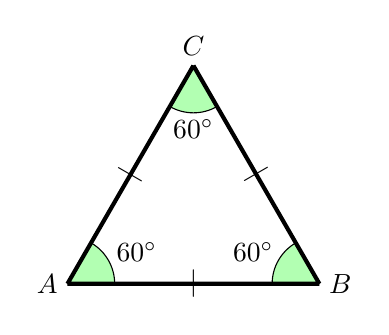
\begin{tikzpicture}[scale=0.8]
                \coordinate[label=left:$A$]  (A) at (0,0);
                \coordinate[label=right:$B$] (B) at (4,0);
                \coordinate[label=above:$C$] (C) at (2,3.464);
                % angle alpha
                \draw[fill=green!30] (0,0) -- (0:0.75cm) arc (0:60:.75cm);
                \draw (1.10cm,0.5cm) node {$60^\circ$};
            
                % angle beta
                \begin{scope}[shift={(4cm,0cm)}]
                    \draw[fill=green!30] (0,0) -- (-180:0.75cm) arc (180:120:0.75cm);
                    \draw (-1.05cm, 0.5cm) node {$60^\circ$};
                \end{scope}
            
                % angle gamma
                \begin{scope}[shift={(60:4)}]
                    \draw[fill=green!30] (0,0) -- (-120:.75cm) arc (-120:-60:.75cm);
                    \draw (-90:1cm) node {$60^\circ$};
                \end{scope}
            
                % the triangle
                \draw [line width=1.5pt] (A) --  node[sloped] {$|$} (B)
                                         (A) --  node[sloped] {$|$} (C)
                                         (B) --  node[sloped] {$|$} (C);
              \end{tikzpicture}
            \label{fig:equilateral_triangle}
    \end{figure}
    %
    \column{0.45\textwidth}
        \begin{align*}
            \overline{AC} &= \overline{BC} = \overline{AB}
            \\
            \angle A &= \angle B = \angle C = 60^\circ
        \end{align*}
    \end{columns}
\end{frame}
%%%%%%%%%%%%%%%%%%%%%%%%%%%%%%%%%%%%%%%%%%%%%%%%
%        SLIDE 
%%%%%%%%%%%%%%%%%%%%%%%%%%%%%%%%%%%%%%%%%%%%%%%%
\subsection{Right Triangle}
\begin{frame}{Right Triangle}
    \begin{itemize}
        \item One angle is right angle ($90^\circ$).
        \item Hypotenuse is the largest side ($c$). It is always opposite of right angle.
        \item The other side is called legs.
        \item \alert{It is very important to identify which one is hypotenuse!!}
    \end{itemize}
    %
    \begin{columns}
    \column{0.45\textwidth}
        \begin{figure}[H]
            \centering
                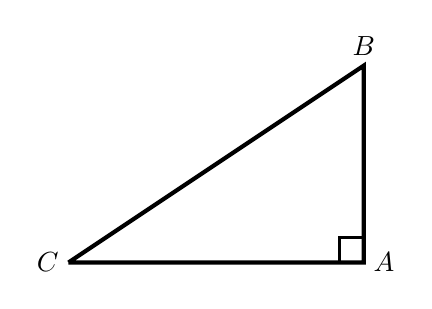
\begin{tikzpicture}[scale=1.25]
                    \coordinate [label=left:$C$]  (C) at (-1.5cm,-1.0cm);
                    \coordinate [label=right:$A$] (A) at (1.5cm,-1.0cm);
                    \coordinate [label=above:$B$] (B) at (1.5cm,1.0cm);
                    \draw [line width=1.5pt] (C) -- (B) -- (A) -- (C);
                    \draw [line width=1pt] (1.25cm,-1.0cm) rectangle (1.5cm,-0.75cm);
                \end{tikzpicture}
            \label{fig:right_triangle}
        \end{figure}
    %
    \column{0.45\textwidth}
        \begin{align*}
            & \text{$\overline{BC}$ is hypotenuse}
            \\
            & \angle A = 90^\circ
        \end{align*}
    \end{columns}    
\end{frame}
%%%%%%%%%%%%%%%%%%%%%%%%%%%%%%%%%%%%%%%%%%%%%%%%
%        SLIDE 
%%%%%%%%%%%%%%%%%%%%%%%%%%%%%%%%%%%%%%%%%%%%%%%%
\subsection{Scalene, Obtuse, and Acute Triangles}
\begin{frame}[t]{Scalene, Obtuse, and Acute Triangles}
    \begin{columns}[t]
    \column{0.25\textwidth}
        \textbf{Scalene:} 
        
        In this triangle, no two sides nor two angles are equal. 
        \begin{figure}[H]
            \centering
                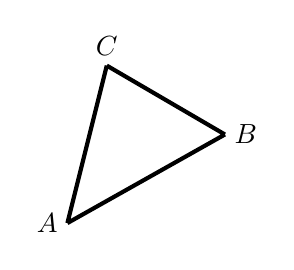
\begin{tikzpicture}[scale=0.5]
                \coordinate[label=left:$A$]  (A) at (0,-1);
                \coordinate[label=right:$B$] (B) at (4,1.25);
                \coordinate[label=above:$C$] (C) at (1,3);
            
                % the triangle
                \draw [line width=1.5pt] (A) --   (B)
                                         (A) --   (C)
                                         (B) --   (C);
              \end{tikzpicture}
            \label{fig:scalene_triangle}
        \end{figure}
    \column{0.33\textwidth}
        \textbf{Obtuse Triangle:} 
        
        One of the angle in this triangle is an obtuse angle; In other words, one angles is between $90^\circ$ and $180^\circ$.
        \begin{figure}[H]
            \centering
                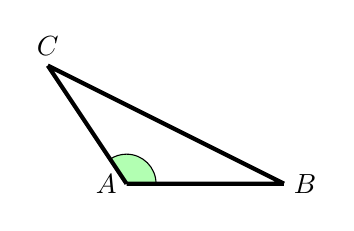
\begin{tikzpicture}[scale=0.5]
                \coordinate[label=left:$A$]  (A) at (0,0);
                \coordinate[label=right:$B$] (B) at (4,0);
                \coordinate[label=above:$C$] (C) at (-2,3);
                % angle alpha
                \draw[fill=green!30] (0,0) -- (0:0.75cm) arc (0:125:.75cm);
                %\draw (0.5cm,1cm) node {$x$};
                
                % the triangle
                \draw [line width=1.5pt] (A) --   (B)
                                         (A) --   (C)
                                         (B) --   (C);
              \end{tikzpicture}
            \label{fig:obtuse_triangle}
        \end{figure}  
    \column{0.33\textwidth}
        \textbf{Acute Triangle}
        
        If all angles are acute angles (less than $90^\circ$), then we have an acute triangle.
        An acute triangle can be equilateral, isosceles or scalene.
        
        \begin{figure}[H]
            \centering
                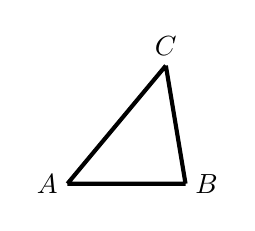
\begin{tikzpicture}[scale=0.5]
                \coordinate[label=left:$A$]  (A) at (0,0);
                \coordinate[label=right:$B$] (B) at (3,0);
                \coordinate[label=above:$C$] (C) at (2.5,3);
            
                % the triangle
                \draw [line width=1.5pt] (A) --   (B)
                                         (A) --   (C)
                                         (B) --   (C);
              \end{tikzpicture}
            \label{fig:acute_triangle}
        \end{figure}
        %
    \end{columns}
\end{frame}
%%%%%%%%%%%%%%%%%%%%%%%%%%%%%%%%%%%%%%%%%%%%%%%%
%        SLIDE 
%%%%%%%%%%%%%%%%%%%%%%%%%%%%%%%%%%%%%%%%%%%%%%%%
\begin{frame}[t]{Example (Missing Angle)}
    \begin{example}
        In an isosceles triangle below, find $\angle x$.
        %
        \begin{figure}[H]
            \centering
                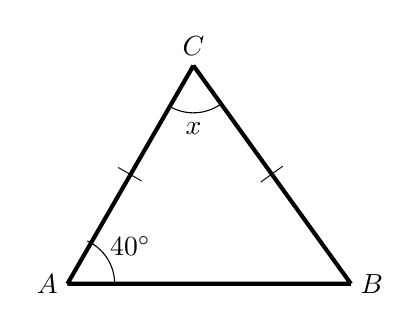
\begin{tikzpicture}[scale=0.8]
                \coordinate[label=left:$A$]  (A) at (0,0);
                \coordinate[label=right:$B$] (B) at (4.5,0);
                \coordinate[label=above:$C$] (C) at (2,3.464);
                %
                \draw(0,0) -- (0:0.75cm) arc (0:65:.75cm);
                \draw (1cm,0.6cm) node {$40^\circ$};
                %
                \begin{scope}[shift={(60:4)}]
                    \draw (0,0) -- (-120:.75cm) arc (-120:-55:.75cm);
                    \draw (-90:1cm) node {$x$};
                \end{scope}
                % triangle
                \draw [line width=1.5pt] (A) --  (B)
                                         (A) -- node[sloped] {$|$} (C)
                                         (B) -- node[sloped] {$|$} (C);
              \end{tikzpicture}
        \end{figure}
    \end{example}
\end{frame}
%%%%%%%%%%%%%%%%%%%%%%%%%%%%%%%%%%%%%%%%%%%%%%%%
%        SLIDE 
%%%%%%%%%%%%%%%%%%%%%%%%%%%%%%%%%%%%%%%%%%%%%%%%
\begin{frame}[t]{Example (Missing Angle)}
    \begin{example}
        Find $\angle x$.
            \begin{figure}[H]
                \centering
                

\tikzset{every picture/.style={line width=0.75pt}} %set default line width to 0.75pt        

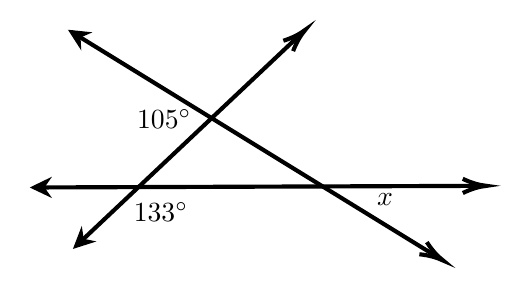
\begin{tikzpicture}[x=0.75pt,y=0.75pt,yscale=-1,xscale=1, scale=0.8]
%uncomment if require: \path (0,216); %set diagram left start at 0, and has height of 216

%Straight Lines [id:da6512016600166057] 
\draw [line width=1.5]    (181,119.99) -- (450,119.01) ;
\draw [shift={(453,119)}, rotate = 539.79] [color={rgb, 255:red, 0; green, 0; blue, 0 }  ][line width=1.5]    (14.21,-4.28) .. controls (9.04,-1.82) and (4.3,-0.39) .. (0,0) .. controls (4.3,0.39) and (9.04,1.82) .. (14.21,4.28)   ;
\draw [shift={(178,120)}, rotate = 359.79] [fill={rgb, 255:red, 0; green, 0; blue, 0 }  ][line width=1.5]  [draw opacity=0] (13.4,-6.43) -- (0,0) -- (13.4,6.44) -- (8.9,0) -- cycle    ;
%Straight Lines [id:da03571309045667914] 
\draw [line width=1.5]    (203.56,26.57) -- (424.44,162.43) ;
\draw [shift={(427,164)}, rotate = 211.59] [color={rgb, 255:red, 0; green, 0; blue, 0 }  ][line width=1.5]    (14.21,-4.28) .. controls (9.04,-1.82) and (4.3,-0.39) .. (0,0) .. controls (4.3,0.39) and (9.04,1.82) .. (14.21,4.28)   ;
\draw [shift={(201,25)}, rotate = 31.59] [fill={rgb, 255:red, 0; green, 0; blue, 0 }  ][line width=1.5]  [draw opacity=0] (13.4,-6.43) -- (0,0) -- (13.4,6.44) -- (8.9,0) -- cycle    ;
%Straight Lines [id:da32587616024700905] 
\draw [line width=1.5]    (206.18,154.94) -- (341.82,27.06) ;
\draw [shift={(344,25)}, rotate = 496.68] [color={rgb, 255:red, 0; green, 0; blue, 0 }  ][line width=1.5]    (14.21,-4.28) .. controls (9.04,-1.82) and (4.3,-0.39) .. (0,0) .. controls (4.3,0.39) and (9.04,1.82) .. (14.21,4.28)   ;
\draw [shift={(204,157)}, rotate = 316.68] [fill={rgb, 255:red, 0; green, 0; blue, 0 }  ][line width=1.5]  [draw opacity=0] (13.4,-6.43) -- (0,0) -- (13.4,6.44) -- (8.9,0) -- cycle    ;

% Text Node
\draw (392,127) node   {$x$};
% Text Node
\draw (257,135) node   {$133^{\circ }$};
% Text Node
\draw (259,79) node   {$105^{\circ }$};


\end{tikzpicture}
            \end{figure}
    \end{example}
\end{frame}

%%%%%%%%%%%%%%%%%%%%%%%%%%%%%%%%%%%%%%%%%%%%%%%%
%        SLIDE 
%%%%%%%%%%%%%%%%%%%%%%%%%%%%%%%%%%%%%%%%%%%%%%%%
\section{Quadrilaterals}
\begin{frame}{Quadrilaterals}
    \begin{itemize}
        \item We will discuss 5 common quadrilateral with some of their basic properties.
        \item Sum of interior angles in a quadrilateral is $360^\circ$.
    \end{itemize}
    %
    \begin{figure}[H]
        \centering
        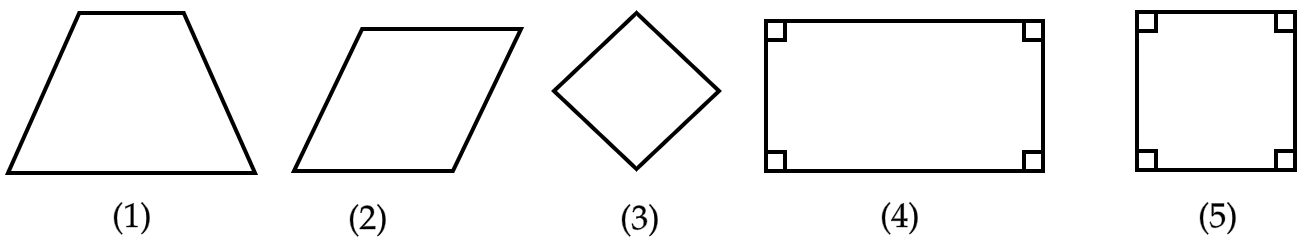
\includegraphics[scale=0.32]{pics/types_quadri.png}
    \end{figure}
\end{frame}
%%%%%%%%%%%%%%%%%%%%%%%%%%%%%%%%%%%%%%%%%%%%%%%%
%        SLIDE 
%%%%%%%%%%%%%%%%%%%%%%%%%%%%%%%%%%%%%%%%%%%%%%%%
\subsection{Trapezoid}
\begin{frame}{Trapezoid}
    \begin{itemize}
        \item Only two sides are parallel. 
        \item Those sides are called \textit{bases}.
    \end{itemize}
    %
    \begin{figure}[H]
        \centering
        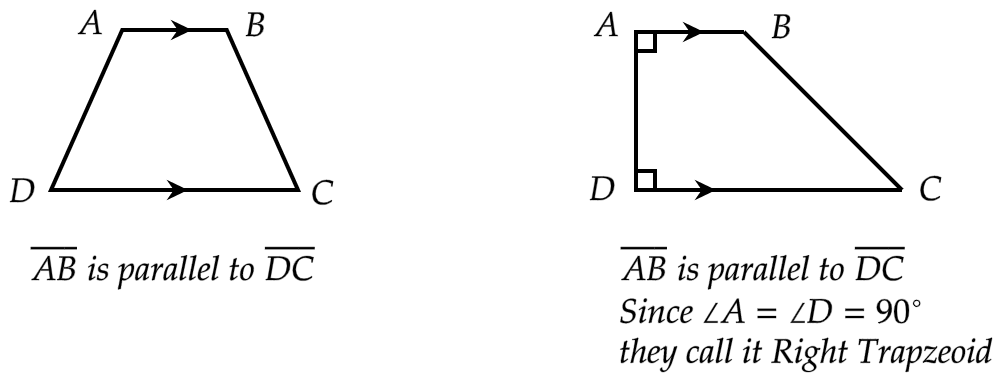
\includegraphics[scale=0.3]{pics/trapezoid.png}
    \end{figure}
\end{frame}
%%%%%%%%%%%%%%%%%%%%%%%%%%%%%%%%%%%%%%%%%%%%%%%%
%        SLIDE 
%%%%%%%%%%%%%%%%%%%%%%%%%%%%%%%%%%%%%%%%%%%%%%%%
\subsection{Parallelogram}
\begin{frame}{Parallelogram}
    \begin{itemize}
        \item Opposite sides are parallel.
        \item Opposite sides are equal.
    \end{itemize}
    %
    \begin{figure}[H]
        \centering
        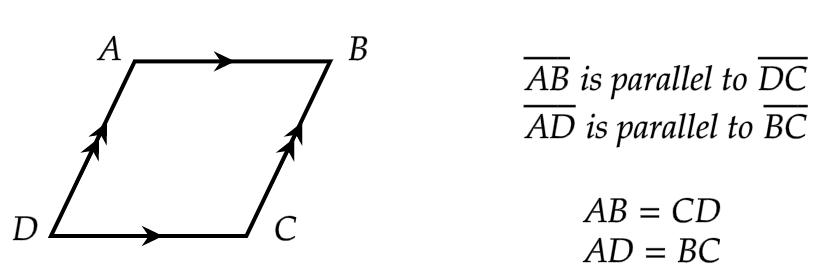
\includegraphics[scale=0.3]{pics/parallelogram.png}
    \end{figure}    
\end{frame}
%%%%%%%%%%%%%%%%%%%%%%%%%%%%%%%%%%%%%%%%%%%%%%%%
%        SLIDE 
%%%%%%%%%%%%%%%%%%%%%%%%%%%%%%%%%%%%%%%%%%%%%%%%
\subsection{Rhombus}
\begin{frame}{Rhombus (Diamond)}
    \begin{itemize}
        \item Opposite sides are parallel.
        \item All sides are equal.
    \end{itemize}
    %
    \begin{figure}[H]
        \centering
        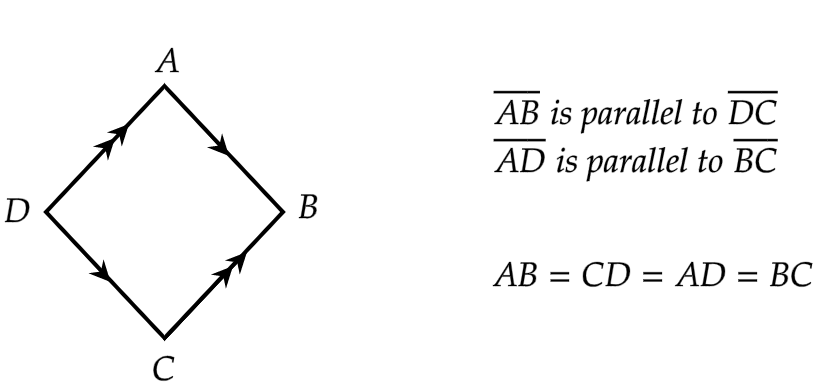
\includegraphics[scale=0.3]{pics/rhombus.png}
    \end{figure} 
\end{frame}
%%%%%%%%%%%%%%%%%%%%%%%%%%%%%%%%%%%%%%%%%%%%%%%%
%        SLIDE 
%%%%%%%%%%%%%%%%%%%%%%%%%%%%%%%%%%%%%%%%%%%%%%%%
\subsection{Rectangle}
\begin{frame}{Rectangle}
    \begin{itemize}
        \item Opposite sides are parallel.
        \item Opposite sides are equal.
        \item All angles are right angles (they are all $90^\circ$).
    \end{itemize}
    %
    \begin{figure}[H]
        \centering
        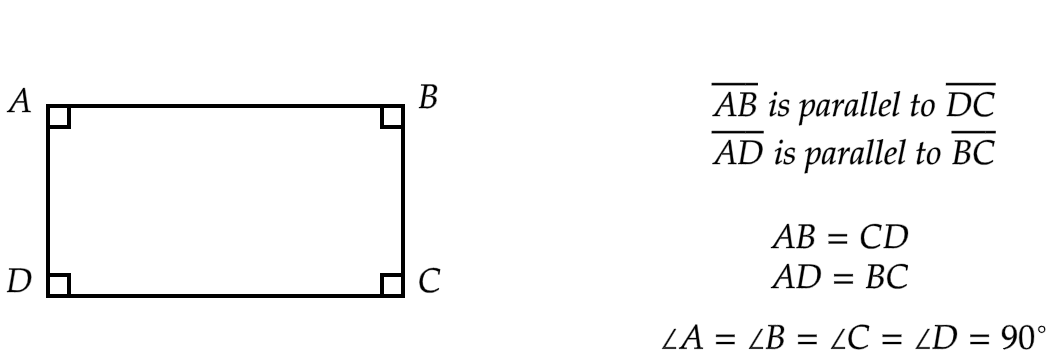
\includegraphics[scale=0.3]{pics/rectangle.png}
    \end{figure}   
\end{frame}
%%%%%%%%%%%%%%%%%%%%%%%%%%%%%%%%%%%%%%%%%%%%%%%%
%        SLIDE 
%%%%%%%%%%%%%%%%%%%%%%%%%%%%%%%%%%%%%%%%%%%%%%%%
\subsection{Square}
\begin{frame}{Square}
    \begin{itemize}
        \item Opposite sides are parallel.
        \item All sides are equal.
        \item All angles are right angles (they are all $90^\circ$).
    \end{itemize}
    %
    \begin{figure}[H]
        \centering
        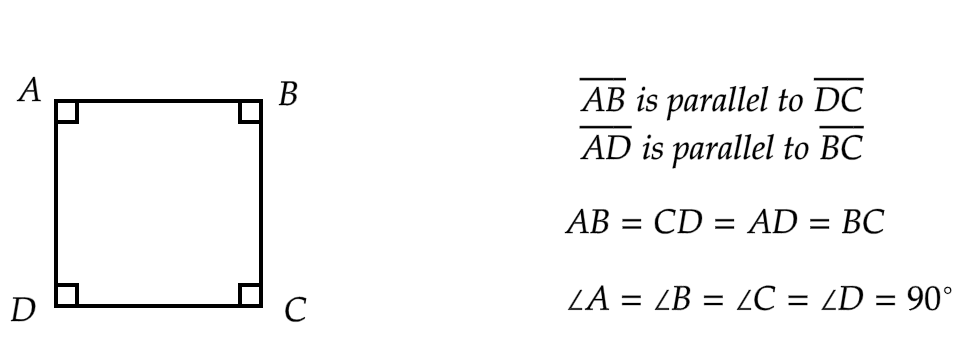
\includegraphics[scale=0.3]{pics/square.png}
    \end{figure}   
\end{frame}
%%%%%%%%%%%%%%%%%%%%%%%%%%%%%%%%%%%%%%%%%%%%%%%%
%        SLIDE 
%%%%%%%%%%%%%%%%%%%%%%%%%%%%%%%%%%%%%%%%%%%%%%%%
\begin{frame}[t]{Example (Find angles)}
    \begin{example}
        \begin{columns}[t]
        %
        \column{0.45\textwidth}
        Trapezoid $ABCD$ is shown below. 
        \begin{enumerate}[(a)]
            \item Determine $\angle x$.
            \item Determine $\angle y$.
        \end{enumerate}
        %
        \column{0.45\textwidth}
        \begin{figure}[H]
            \centering
            

\tikzset{every picture/.style={line width=0.75pt}} %set default line width to 0.75pt        

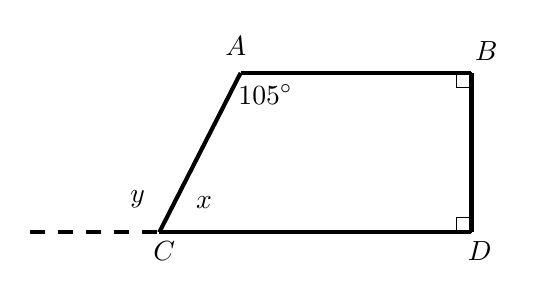
\begin{tikzpicture}[x=0.75pt,y=0.75pt,yscale=-1,xscale=1, scale=0.8]
%uncomment if require: \path (0,218); %set diagram left start at 0, and has height of 218

%Shape: Rectangle [id:dp392879367849994] 
\draw   (418,146) -- (427,146) -- (427,155) -- (418,155) -- cycle ;
%Shape: Rectangle [id:dp28556743489112235] 
\draw   (418,59) -- (427,59) -- (427,68) -- (418,68) -- cycle ;
%Straight Lines [id:da15725270794626356] 
\draw [line width=1.5]    (427,155) -- (239,155) ;


%Straight Lines [id:da6108314492525089] 
\draw [line width=1.5]    (427,155) -- (427,59) ;


%Straight Lines [id:da21099235794946036] 
\draw [line width=1.5]    (288,59) -- (427,59) ;


%Straight Lines [id:da9882398763880909] 
\draw [line width=1.5]    (239,155) -- (288,59) ;


%Straight Lines [id:da2719389491415545] 
\draw [line width=1.5]  [dash pattern={on 5.63pt off 4.5pt}]  (161,155) -- (239,155) ;



% Text Node
\draw (285,43) node   {$A$};
% Text Node
\draw (436,46) node   {$B$};
% Text Node
\draw (242,166) node   {$C$};
% Text Node
\draw (432,166) node   {$D$};
% Text Node
\draw (303,72) node   {$105^{\circ }$};
% Text Node
\draw (266,137) node   {$x$};
% Text Node
\draw (226,135) node   {$y$};


\end{tikzpicture}
        \end{figure}
        %
        \end{columns}
    \end{example}
\end{frame}
% PART 3 (SECTION 8.3)
\part{Section 8.3}
%%%%%%%%%%%%%%%%%%%%%%%%%%%%%%%%%%%%%%%
\begin{transitionframe}
    \begin{center}
    { 
        \Huge \textcolor{white}{\textbf{Area and Perimeter}}
        \\[-1em]
        \noindent\textcolor{white}{\rule{12cm}{0.4pt}}
        
        %\large \textcolor{white}{Section 8.3}
    }
    \end{center}
\end{transitionframe}
%%%%%%%%%%%%%%%%%%%%%%%%%%%%%%%%%%%%%%%
%        SLIDE 
%%%%%%%%%%%%%%%%%%%%%%%%%%%%%%%%%%%%%%%
\begin{frame}{Outline}
            \tableofcontents[part=3]
\end{frame}
%%%%%%%%%%%%%%%%%%%%%%%%%%%%%%%%%%%%%%%
%        SLIDE 
%%%%%%%%%%%%%%%%%%%%%%%%%%%%%%%%%%%%%%%
\section{Perimeter}
\begin{frame}[t]{Perimeter}
    \begin{columns}
    %
    \column{0.45\textwidth}
    %
    \begin{block}{Definition}
        Perimeter, denoted $P$, is the distance around the outside of a shape.
    \end{block}
    %
    \begin{itemize}
        \item In other words, the sum of lengths of the sides of a shape.
        \item The unit of the perimeter is the same as the unit of the length such as inches (in), feet (ft), meter (m), millimeter (mm), centimeter (cm) and so forth.
    \end{itemize}
    %
    \column{0.45\textwidth}
    \textbf{Example:}
    \begin{figure}[H]
        \centering
        

\tikzset{every picture/.style={line width=0.75pt}} %set default line width to 0.75pt        

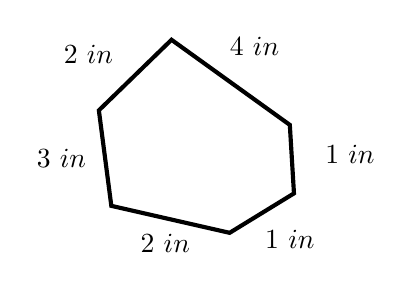
\begin{tikzpicture}[x=0.75pt,y=0.75pt,yscale=-1,xscale=1]
%uncomment if require: \path (0,167); %set diagram left start at 0, and has height of 167

%Shape: Polygon [id:ds1989494780526837] 
\draw  [line width=1.5]  (299,40) -- (356,81) -- (358,114) -- (327,133) -- (270,120) -- (264,74) -- cycle ;

% Text Node
\draw (259,47) node   {$2\ in$};
% Text Node
\draw (296,138) node   {$2\ in$};
% Text Node
\draw (246,97) node   {$3\ in$};
% Text Node
\draw (339,43) node   {$4\ in$};
% Text Node
\draw (385,95) node   {$1\ in$};
% Text Node
\draw (356,136) node   {$1\ in$};


\end{tikzpicture}
        \label{fig:perimeter}
    \end{figure}
    %
    \[
        P = 1+1+2+2+3+4 = 13\ \mathrm{in}
    \]
    \end{columns}
\end{frame}
%%%%%%%%%%%%%%%%%%%%%%%%%%%%%%%%%%%%%%%
%        SLIDE 
%%%%%%%%%%%%%%%%%%%%%%%%%%%%%%%%%%%%%%%
\begin{frame}[t]{Example (Find the perimeter)}
    \begin{example}
        Find the perimeter of the following parallelogram.
        %
        \begin{figure}[H]
            \centering
            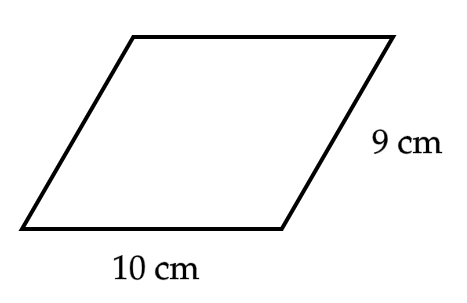
\includegraphics[scale=0.25]{pics/perimeter_1.png}
        \end{figure}
    \end{example}
    %
\end{frame}
%%%%%%%%%%%%%%%%%%%%%%%%%%%%%%%%%%%%%%%
%        SLIDE 
%%%%%%%%%%%%%%%%%%%%%%%%%%%%%%%%%%%%%%%
\section{Area}
\begin{frame}[t]{Area}
    \begin{columns}[t]
    %
    \column{0.45\textwidth}
    \begin{block}{Definition}
        An area, denoted $A$, is the measure of region within the boundaries of a shape.
    \end{block}
    %
    \begin{itemize}
        \item In other words, area is the size of surface insides a shape.
    \end{itemize}
    %
    \column{0.45\textwidth}
    \begin{figure}[H]
        \centering
        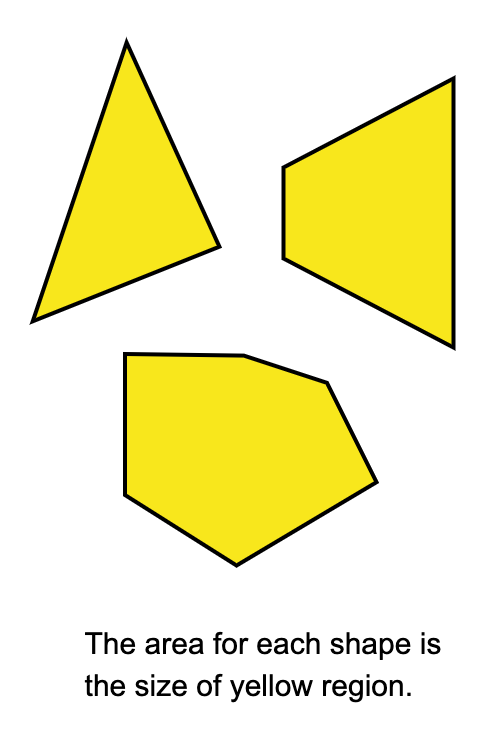
\includegraphics[width=0.6\textwidth]{pics/area_def.png}
    \end{figure}        
    \end{columns}
\end{frame}
%%%%%%%%%%%%%%%%%%%%%%%%%%%%%%%%%%%%%%%
%        SLIDE 
%%%%%%%%%%%%%%%%%%%%%%%%%%%%%%%%%%%%%%%
\subsection{How to Measure the Area?}
\begin{frame}{How to Measure the Area?}
    \begin{itemize}
        \item Area is basically the number of \textit{square units} that covers a shape.
    \end{itemize}
    %
    \begin{figure}[H]
        \centering
        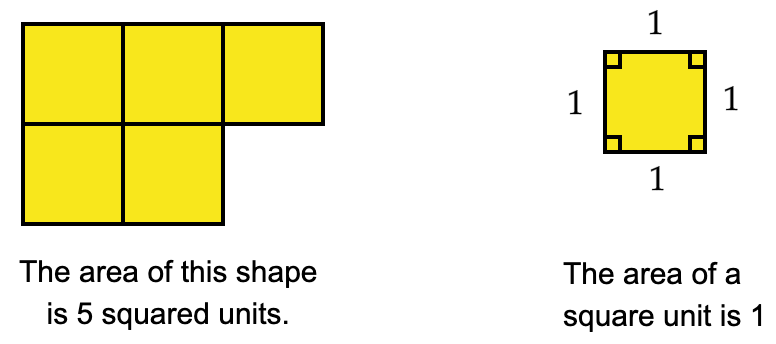
\includegraphics[scale=0.3]{pics/square_units.png}
    \end{figure}
    %
    \begin{itemize}
        \item The area is measure in squared units like square inches ($\mathrm{in^2}$), squared feet ($\mathrm{ft^2}$), squared cm ($\mathrm{cm^2}$), and so on.
        \item Using square units, we eventually develop a formula to calculate the area.
    \end{itemize}
\end{frame}
%%%%%%%%%%%%%%%%%%%%%%%%%%%%%%%%%%%%%%%
%        SLIDE 
%%%%%%%%%%%%%%%%%%%%%%%%%%%%%%%%%%%%%%%
\subsection{Area of a Rectangle}
\begin{frame}[t]{Area of a Rectangle}
    \begin{columns}[t]
    \column{0.45\textwidth}
    \begin{itemize}
        \item To find the area of a rectangle, we will find it using the square units. 
        \item As it is shown in Figure on the right, there is a relationship between the area of a rectangle, its length ($\ell$), and its width ($w$).
    \end{itemize}
    %
    \begin{block}{Formula}
        The area of a rectangle with length $\ell$ and width $w$ is equal to
        \[ A = \ell\cdot w \]
    \end{block}
    %
    \column{0.45\textwidth}
    %
    \begin{figure}[H]
        \centering
        

\tikzset{every picture/.style={line width=0.75pt}} %set default line width to 0.75pt        

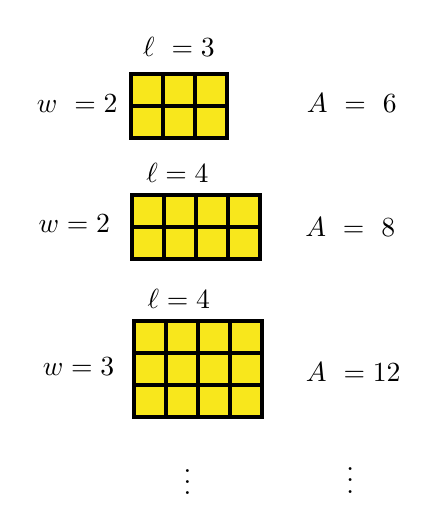
\begin{tikzpicture}[x=0.75pt,y=0.75pt,yscale=-1,xscale=1,scale=0.7]
%uncomment if require: \path (0,338); %set diagram left start at 0, and has height of 338

%Shape: Square [id:dp38271822688596946] 
\draw  [fill={rgb, 255:red, 248; green, 231; blue, 28 }  ,fill opacity=1 ][line width=1.5]  (189,34) -- (211,34) -- (211,56) -- (189,56) -- cycle ;
%Shape: Square [id:dp8679439248883813] 
\draw  [fill={rgb, 255:red, 248; green, 231; blue, 28 }  ,fill opacity=1 ][line width=1.5]  (211,34) -- (233,34) -- (233,56) -- (211,56) -- cycle ;
%Shape: Square [id:dp3558050933364425] 
\draw  [fill={rgb, 255:red, 248; green, 231; blue, 28 }  ,fill opacity=1 ][line width=1.5]  (233,34) -- (255,34) -- (255,56) -- (233,56) -- cycle ;
%Shape: Square [id:dp8748116538918442] 
\draw  [fill={rgb, 255:red, 248; green, 231; blue, 28 }  ,fill opacity=1 ][line width=1.5]  (189,56) -- (211,56) -- (211,78) -- (189,78) -- cycle ;
%Shape: Square [id:dp06759803167989387] 
\draw  [fill={rgb, 255:red, 248; green, 231; blue, 28 }  ,fill opacity=1 ][line width=1.5]  (211,56) -- (233,56) -- (233,78) -- (211,78) -- cycle ;
%Shape: Square [id:dp3172857824306643] 
\draw  [fill={rgb, 255:red, 248; green, 231; blue, 28 }  ,fill opacity=1 ][line width=1.5]  (233,56) -- (255,56) -- (255,78) -- (233,78) -- cycle ;
%Shape: Square [id:dp9771058827150725] 
\draw  [fill={rgb, 255:red, 248; green, 231; blue, 28 }  ,fill opacity=1 ][line width=1.5]  (190,117) -- (212,117) -- (212,139) -- (190,139) -- cycle ;
%Shape: Square [id:dp10490248151810566] 
\draw  [fill={rgb, 255:red, 248; green, 231; blue, 28 }  ,fill opacity=1 ][line width=1.5]  (212,117) -- (234,117) -- (234,139) -- (212,139) -- cycle ;
%Shape: Square [id:dp8310609107018645] 
\draw  [fill={rgb, 255:red, 248; green, 231; blue, 28 }  ,fill opacity=1 ][line width=1.5]  (234,117) -- (256,117) -- (256,139) -- (234,139) -- cycle ;
%Shape: Square [id:dp5473468611089647] 
\draw  [fill={rgb, 255:red, 248; green, 231; blue, 28 }  ,fill opacity=1 ][line width=1.5]  (190,139) -- (212,139) -- (212,161) -- (190,161) -- cycle ;
%Shape: Square [id:dp12474790550517523] 
\draw  [fill={rgb, 255:red, 248; green, 231; blue, 28 }  ,fill opacity=1 ][line width=1.5]  (212,139) -- (234,139) -- (234,161) -- (212,161) -- cycle ;
%Shape: Square [id:dp34696767252717375] 
\draw  [fill={rgb, 255:red, 248; green, 231; blue, 28 }  ,fill opacity=1 ][line width=1.5]  (234,139) -- (256,139) -- (256,161) -- (234,161) -- cycle ;
%Shape: Square [id:dp13867107777486232] 
\draw  [fill={rgb, 255:red, 248; green, 231; blue, 28 }  ,fill opacity=1 ][line width=1.5]  (256,117) -- (278,117) -- (278,139) -- (256,139) -- cycle ;
%Shape: Square [id:dp5849236655713153] 
\draw  [fill={rgb, 255:red, 248; green, 231; blue, 28 }  ,fill opacity=1 ][line width=1.5]  (256,139) -- (278,139) -- (278,161) -- (256,161) -- cycle ;
%Shape: Square [id:dp7422021146428393] 
\draw  [fill={rgb, 255:red, 248; green, 231; blue, 28 }  ,fill opacity=1 ][line width=1.5]  (191,204) -- (213,204) -- (213,226) -- (191,226) -- cycle ;
%Shape: Square [id:dp8646869287162122] 
\draw  [fill={rgb, 255:red, 248; green, 231; blue, 28 }  ,fill opacity=1 ][line width=1.5]  (213,204) -- (235,204) -- (235,226) -- (213,226) -- cycle ;
%Shape: Square [id:dp436268216442143] 
\draw  [fill={rgb, 255:red, 248; green, 231; blue, 28 }  ,fill opacity=1 ][line width=1.5]  (235,204) -- (257,204) -- (257,226) -- (235,226) -- cycle ;
%Shape: Square [id:dp40039453862710905] 
\draw  [fill={rgb, 255:red, 248; green, 231; blue, 28 }  ,fill opacity=1 ][line width=1.5]  (191,226) -- (213,226) -- (213,248) -- (191,248) -- cycle ;
%Shape: Square [id:dp34900812081397414] 
\draw  [fill={rgb, 255:red, 248; green, 231; blue, 28 }  ,fill opacity=1 ][line width=1.5]  (213,226) -- (235,226) -- (235,248) -- (213,248) -- cycle ;
%Shape: Square [id:dp6134216351528443] 
\draw  [fill={rgb, 255:red, 248; green, 231; blue, 28 }  ,fill opacity=1 ][line width=1.5]  (235,226) -- (257,226) -- (257,248) -- (235,248) -- cycle ;
%Shape: Square [id:dp2972790637499185] 
\draw  [fill={rgb, 255:red, 248; green, 231; blue, 28 }  ,fill opacity=1 ][line width=1.5]  (257,204) -- (279,204) -- (279,226) -- (257,226) -- cycle ;
%Shape: Square [id:dp6141269163406937] 
\draw  [fill={rgb, 255:red, 248; green, 231; blue, 28 }  ,fill opacity=1 ][line width=1.5]  (257,226) -- (279,226) -- (279,248) -- (257,248) -- cycle ;
%Shape: Square [id:dp04871647434354265] 
\draw  [fill={rgb, 255:red, 248; green, 231; blue, 28 }  ,fill opacity=1 ][line width=1.5]  (191,248) -- (213,248) -- (213,270) -- (191,270) -- cycle ;
%Shape: Square [id:dp6693543844606036] 
\draw  [fill={rgb, 255:red, 248; green, 231; blue, 28 }  ,fill opacity=1 ][line width=1.5]  (213,248) -- (235,248) -- (235,270) -- (213,270) -- cycle ;
%Shape: Square [id:dp25950883575769756] 
\draw  [fill={rgb, 255:red, 248; green, 231; blue, 28 }  ,fill opacity=1 ][line width=1.5]  (235,248) -- (257,248) -- (257,270) -- (235,270) -- cycle ;
%Shape: Square [id:dp5668503605566757] 
\draw  [fill={rgb, 255:red, 248; green, 231; blue, 28 }  ,fill opacity=1 ][line width=1.5]  (257,248) -- (279,248) -- (279,270) -- (257,270) -- cycle ;

% Text Node
\draw (222,15) node   {$\ell \ =3$};
% Text Node
\draw (152,54) node   {$w\ =2$};
% Text Node
\draw (341,54) node   {$A\ =\ 6$};
% Text Node
\draw (221,102) node   {$\ell =4$};
% Text Node
\draw (150,137) node   {$w=2$};
% Text Node
\draw (340,139) node   {$A\ =\ 8$};
% Text Node
\draw (222,189) node   {$\ell =4$};
% Text Node
\draw (153,235) node   {$w=3$};
% Text Node
\draw (342,239) node   {$A\ =12$};
% Text Node
\draw (228,309) node   {$\boldsymbol{\vdots }$};
% Text Node
\draw (340,308) node   {$\boldsymbol{\vdots }$};


\end{tikzpicture}
    \end{figure}
    \end{columns}
\end{frame}
%%%%%%%%%%%%%%%%%%%%%%%%%%%%%%%%%%%%%%%
%        SLIDE 
%%%%%%%%%%%%%%%%%%%%%%%%%%%%%%%%%%%%%%%
\subsection{Area of a Square}
\begin{frame}[t]{Area of a Square}
    \begin{columns}
    \column{0.45\textwidth}
    \begin{itemize}
        \item A square is a special case of a rectangle in which both length and width are equal in length.
        \item Let's say they both are equal to $s$.
        \item Using the rectangle formula, one can easily find the area of a square.
    \end{itemize}
    %
    \begin{block}{Formula}
        If a side of square is $s$, then its area can be found as follow:
        \[ A = s^2\]
    \end{block}
    %
    \column{0.45\textwidth}
    \begin{figure}[H]
        \centering
        

\tikzset{every picture/.style={line width=0.75pt}} %set default line width to 0.75pt        

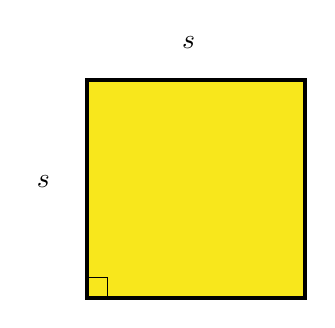
\begin{tikzpicture}[x=0.75pt,y=0.75pt,yscale=-1,xscale=1]
%uncomment if require: \path (0,167); %set diagram left start at 0, and has height of 167

%Shape: Square [id:dp9958510811050907] 
\draw  [fill={rgb, 255:red, 248; green, 231; blue, 28 }  ,fill opacity=1 ][line width=1.5]  (207,37) -- (312,37) -- (312,142) -- (207,142) -- cycle ;
%Shape: Square [id:dp2209502611968972] 
\draw   (207,132) -- (217,132) -- (217,142) -- (207,142) -- cycle ;

% Text Node
\draw (186,86) node   {$s$};
% Text Node
\draw (256,19) node   {$s$};
% Text Node
% \draw (411,87) node   {$ \begin{array}{l}
% \boldsymbol{A\ =\ s^{2}}\\
% \\
% \boldsymbol{P\ =\ 4s}
% \end{array}$};


\end{tikzpicture}
    \end{figure}    
    \end{columns}
\end{frame}
%%%%%%%%%%%%%%%%%%%%%%%%%%%%%%%%%%%%%%%
%        SLIDE 
%%%%%%%%%%%%%%%%%%%%%%%%%%%%%%%%%%%%%%%
\begin{frame}[t]{Example (Find Area and Perimeter)}
    \begin{example}
        Find the area and perimeter of each shape.
        %
        \begin{figure}[H]
            \centering
            

\tikzset{every picture/.style={line width=0.75pt}} %set default line width to 0.75pt        

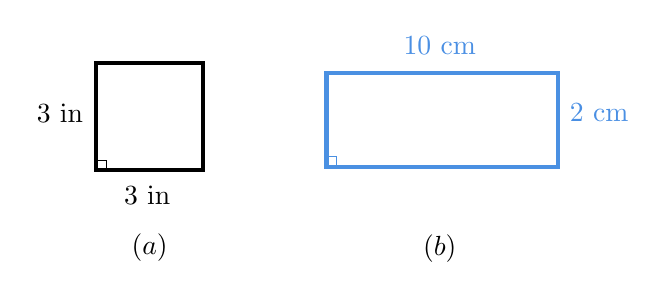
\begin{tikzpicture}[x=0.75pt,y=0.75pt,yscale=-1,xscale=1, scale=0.6]
%uncomment if require: \path (0,218); %set diagram left start at 0, and has height of 218

%Shape: Square [id:dp9958510811050907] 
\draw  [line width=1.5]  (135,45) -- (221,45) -- (221,131) -- (135,131) -- cycle ;
%Shape: Square [id:dp2209502611968972] 
\draw   (135,122.81) -- (143.19,122.81) -- (143.19,131) -- (135,131) -- cycle ;
%Shape: Rectangle [id:dp27912537729912623] 
\draw  [color={rgb, 255:red, 74; green, 144; blue, 226 }  ,draw opacity=1 ][line width=1.5]  (320,53) -- (506,53) -- (506,128) -- (320,128) -- cycle ;
%Shape: Square [id:dp059563169319218456] 
\draw  [color={rgb, 255:red, 74; green, 144; blue, 226 }  ,draw opacity=1 ] (320,119.81) -- (328.19,119.81) -- (328.19,128) -- (320,128) -- cycle ;

% Text Node
\draw (106,85) node   {$3\text{ in}$};
% Text Node
\draw (176,151) node   {$3\text{ in}$};
% Text Node
\draw (178,193) node   {$( a)$};
% Text Node
\draw (411,31) node   {$\textcolor[rgb]{0.29,0.56,0.89}{10\ \text{cm}}$};
% Text Node
\draw (539,85) node   {$\textcolor[rgb]{0.29,0.56,0.89}{2\ }\textcolor[rgb]{0.29,0.56,0.89}{\text{cm}}$};
% Text Node
\draw (411,194) node   {$( b)$};


\end{tikzpicture}
        \end{figure}
    \end{example}
\end{frame}

%%%%%%%%%%%%%%%%%%%%%%%%%%%%%%%%%%%%%%%
%        SLIDE 
%%%%%%%%%%%%%%%%%%%%%%%%%%%%%%%%%%%%%%%
\subsection{Area of a Parallelogram}
\begin{frame}{Area of a Parallelogram}
    \begin{columns}
    %
    \column{0.45\textwidth}
    \begin{itemize}
        \item Height of a parallelogram, $h$, is the distance between two parallel sides.
        \item Those parallel sides are called bases and we showed them with $b$.
        \item It can be proven the area of a parallelogram is height times its base.
    \end{itemize}
    %
    \begin{block}{Formula}
        If $h$ is height of the parallelogram and $b$ is the side which height is perpendicular to it, then the area of the parallelogram can be found as follow:
        \[ A = b \cdot h\] 
    \end{block}
    %
    \column{0.45\textwidth}
    \begin{figure}[H]
        \centering
        

\tikzset{every picture/.style={line width=0.75pt}} %set default line width to 0.75pt        

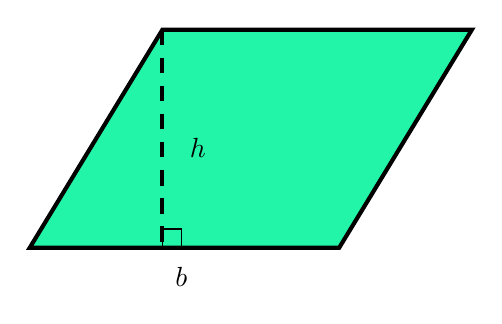
\begin{tikzpicture}[x=0.75pt,y=0.75pt,yscale=-1,xscale=1]
%uncomment if require: \path (0,187); %set diagram left start at 0, and has height of 187

%Shape: Parallelogram [id:dp6701686139689902] 
\draw  [fill={rgb, 255:red, 35; green, 245; blue, 168 }   ,fill opacity=1 ][line width=1.5]  (276.9,48) -- (426,48) -- (362.1,153) -- (213,153) -- cycle ;
%Straight Lines [id:da38364165600367084] 
\draw [line width=1.5]  [dash pattern={on 5.63pt off 4.5pt}]  (276.9,48) -- (276.9,153) ;


%Shape: Square [id:dp885829648238055] 
\draw   (276.9,144) -- (285.9,144) -- (285.9,153) -- (276.9,153) -- cycle ;

% Text Node
\draw (286,167) node   {$b$};
% Text Node
\draw (294,105) node   {$h$};


\end{tikzpicture}
    \end{figure}
    \end{columns}
\end{frame}
%%%%%%%%%%%%%%%%%%%%%%%%%%%%%%%%%%%%%%%
%        SLIDE 
%%%%%%%%%%%%%%%%%%%%%%%%%%%%%%%%%%%%%%%
\subsection{Area of a Triangle}
\begin{frame}{Area of a Triangle}
    \begin{columns}
    \column{0.45\textwidth}
        \begin{itemize}
            \item Two triangle make a parallelogram. 
            \item So the area of a triangle is half of a parallelogram with same base and height.
        \end{itemize}
        %
        \begin{block}{Formula}
            If $h$ is distance from one vertex to the side $b$ (called base), then the area of a triangle can be found using the following formula:
            \[  A = \frac{b\cdot h}{2} \]
        \end{block}
        %
        \column{0.45\textwidth}
    \begin{figure}[H]
        \centering
        

\tikzset{every picture/.style={line width=0.75pt}} %set default line width to 0.75pt        

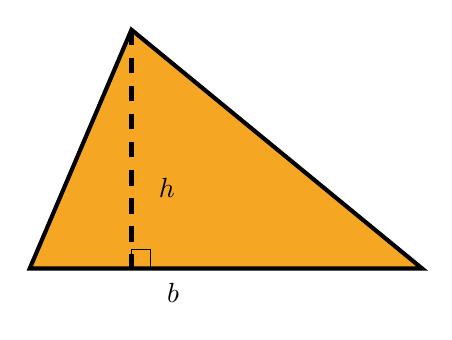
\begin{tikzpicture}[x=0.75pt,y=0.75pt,yscale=-1,xscale=1]
%uncomment if require: \path (0,200); %set diagram left start at 0, and has height of 200

%Shape: Triangle [id:dp48354767803270016] 
\draw  [fill={rgb, 255:red, 245; green, 166; blue, 35 }  ,fill opacity=1 ][line width=1.5]  (277,45) -- (417,160) -- (228,160) -- cycle ;
%Straight Lines [id:da38364165600367084] 
\draw [line width=1.5]  [dash pattern={on 5.63pt off 4.5pt}]  (277,45) -- (277,160) ;


%Shape: Square [id:dp885829648238055] 
\draw   (277,151) -- (286,151) -- (286,160) -- (277,160) -- cycle ;

% Text Node
\draw (297,172) node   {$b$};
% Text Node
\draw (294,121) node   {$h$};
% Text Node


\end{tikzpicture}
    \end{figure}        
    \end{columns}
\end{frame}
%%%%%%%%%%%%%%%%%%%%%%%%%%%%%%%%%%%%%%%
%        SLIDE 
%%%%%%%%%%%%%%%%%%%%%%%%%%%%%%%%%%%%%%%
\begin{frame}{Area of a Triangle (Cont'd)}
    \begin{itemize}
        \item For right triangle, we can consider on leg as a height and the other leg as a base (Figure a).
        \item In addition, one can draw a perpendicular line to the hypotenuse. In this case, the perpendicular line is our height and hypotenuse is our base (Figure b)
    \end{itemize}
    %
    \begin{figure}[H]
        \centering
        

\tikzset{every picture/.style={line width=0.75pt}} %set default line width to 0.75pt        

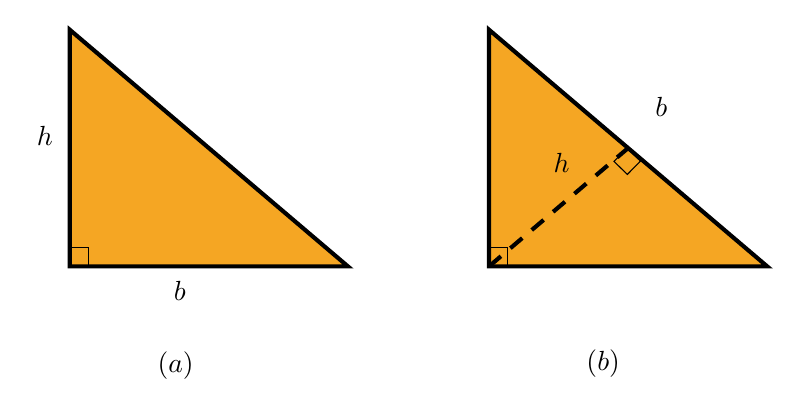
\begin{tikzpicture}[x=0.75pt,y=0.75pt,yscale=-1,xscale=1]
%uncomment if require: \path (0,256); %set diagram left start at 0, and has height of 256

%Shape: Right Triangle [id:dp7083168248857548] 
\draw  [fill={rgb, 255:red, 245; green, 166; blue, 35 }  ,fill opacity=1 ][line width=1.5]  (178,68) -- (312,182) -- (178,182) -- cycle ;
%Shape: Square [id:dp9879546899101135] 
\draw   (178,173) -- (187,173) -- (187,182) -- (178,182) -- cycle ;
%Shape: Right Triangle [id:dp9630416737865424] 
\draw  [fill={rgb, 255:red, 245; green, 166; blue, 35 }  ,fill opacity=1 ][line width=1.5]  (380,68) -- (514,182) -- (380,182) -- cycle ;
%Shape: Square [id:dp12336196242449993] 
\draw   (380,173) -- (389,173) -- (389,182) -- (380,182) -- cycle ;
%Straight Lines [id:da207575097514602] 
\draw [line width=1.5]  [dash pattern={on 5.63pt off 4.5pt}]  (380,182) -- (447,125) ;


%Shape: Square [id:dp9229345478868127] 
\draw   (440.2,131.42) -- (446.5,124.99) -- (452.93,131.28) -- (446.63,137.71) -- cycle ;

% Text Node
\draw (231,194) node   {$b$};
% Text Node
\draw (166,119) node   {$h$};;
% Text Node
\draw (463,105) node   {$b$};
% Text Node
\draw (415,132) node   {$h$};
% Text Node
\draw (229,230) node   {$( a)$};
% Text Node
\draw (435,229) node   {$( b)$};


\end{tikzpicture}
    \end{figure} 
\end{frame}
%%%%%%%%%%%%%%%%%%%%%%%%%%%%%%%%%%%%%%%
%        SLIDE 
%%%%%%%%%%%%%%%%%%%%%%%%%%%%%%%%%%%%%%%
\begin{frame}[t]{Example (Find Area)}
    \begin{example}
        Find the area of each shape.
        %
        \begin{figure}[H]
            \centering
            

\tikzset{every picture/.style={line width=0.75pt}} %set default line width to 0.75pt        

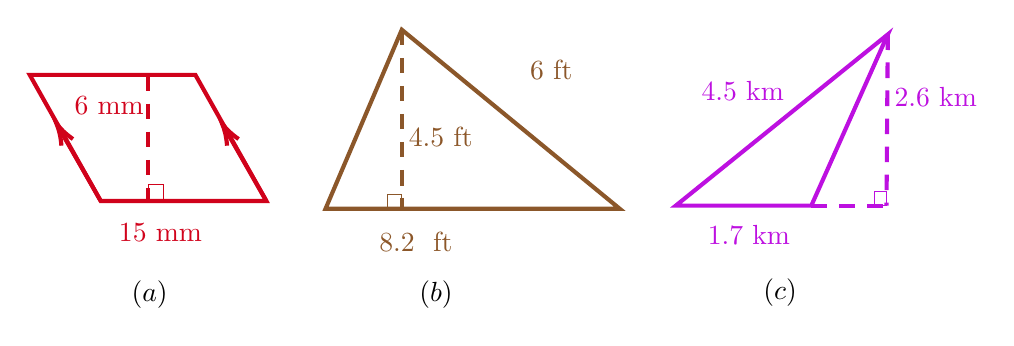
\begin{tikzpicture}[x=0.75pt,y=0.75pt,yscale=-1,xscale=1, scale=0.75]
%uncomment if require: \path (0,230); %set diagram left start at 0, and has height of 230

%Shape: Parallelogram [id:dp4045973963325873] 
\draw  [color={rgb, 255:red, 208; green, 2; blue, 27 }  ,draw opacity=1 ][line width=1.5]  (147.4,59) -- (41,59) -- (86.6,140) -- (193,140) -- cycle ;
%Straight Lines [id:da9796665582380797] 
\draw [color={rgb, 255:red, 208; green, 2; blue, 27 }  ,draw opacity=1 ][line width=1.5]  [dash pattern={on 5.63pt off 4.5pt}]  (117,59.5) -- (117,139.5) ;


%Shape: Square [id:dp06920862972284914] 
\draw  [color={rgb, 255:red, 208; green, 2; blue, 27 }  ,draw opacity=1 ] (117,129.5) -- (127,129.5) -- (127,139.5) -- (117,139.5) -- cycle ;
%Shape: Triangle [id:dp08961522547508038] 
\draw  [color={rgb, 255:red, 139; green, 87; blue, 42 }  ,draw opacity=1 ][line width=1.5]  (280,30) -- (420,145) -- (231,145) -- cycle ;
%Straight Lines [id:da8427678719260143] 
\draw [color={rgb, 255:red, 139; green, 87; blue, 42 }  ,draw opacity=1 ][line width=1.5]  [dash pattern={on 5.63pt off 4.5pt}]  (280,30) -- (280,145) ;


%Shape: Square [id:dp08529804115971995] 
\draw  [color={rgb, 255:red, 139; green, 87; blue, 42 }  ,draw opacity=1 ] (271,136) -- (280,136) -- (280,145) -- (271,145) -- cycle ;
%Shape: Polygon [id:ds9967185060442834] 
\draw  [color={rgb, 255:red, 189; green, 16; blue, 224 }  ,draw opacity=1 ][line width=1.5]  (456,143) -- (543.08,143) -- (592.22,33) -- cycle ;
%Straight Lines [id:da1558061082869422] 
\draw [color={rgb, 255:red, 189; green, 16; blue, 224 }  ,draw opacity=1 ][line width=1.5]  [dash pattern={on 5.63pt off 4.5pt}]  (592.22,33) -- (591.36,143) ;


%Straight Lines [id:da7378491629676467] 
\draw [color={rgb, 255:red, 189; green, 16; blue, 224 }  ,draw opacity=1 ][line width=1.5]  [dash pattern={on 5.63pt off 4.5pt}]  (543.08,143) -- (591.36,143) ;


%Shape: Rectangle [id:dp5477304566759069] 
\draw  [color={rgb, 255:red, 189; green, 16; blue, 224 }  ,draw opacity=1 ] (591.36,134) -- (583.6,134) -- (583.6,143) -- (591.36,143) -- cycle ;
%Straight Lines [id:da6859428859669638] 
\draw [color={rgb, 255:red, 208; green, 2; blue, 27 }  ,draw opacity=1 ][line width=1.5]    (86.6,140) -- (59.49,92.6) ;
\draw [shift={(58,90)}, rotate = 420.23] [color={rgb, 255:red, 208; green, 2; blue, 27 }  ,draw opacity=1 ][line width=1.5]    (14.21,-4.28) .. controls (9.04,-1.82) and (4.3,-0.39) .. (0,0) .. controls (4.3,0.39) and (9.04,1.82) .. (14.21,4.28)   ;

%Straight Lines [id:da26032096428140505] 
\draw [color={rgb, 255:red, 208; green, 2; blue, 27 }  ,draw opacity=1 ][line width=1.5]    (193,140) -- (165.89,92.6) ;
\draw [shift={(164.4,90)}, rotate = 420.23] [color={rgb, 255:red, 208; green, 2; blue, 27 }  ,draw opacity=1 ][line width=1.5]    (14.21,-4.28) .. controls (9.04,-1.82) and (4.3,-0.39) .. (0,0) .. controls (4.3,0.39) and (9.04,1.82) .. (14.21,4.28)   ;


% Text Node
\draw (92,79) node   {$\textcolor[rgb]{0.82,0.01,0.11}{6\ \text{mm}}$};
% Text Node
\draw (125,160) node   {$\textcolor[rgb]{0.82,0.01,0.11}{15\ }\textcolor[rgb]{0.82,0.01,0.11}{\text{mm}}$};
% Text Node
\draw (118,200) node   {$( a)$};
% Text Node
\draw (289,166) node   {$\textcolor[rgb]{0.55,0.34,0.16}{8.2\ \text{ ft}}$};
% Text Node
\draw (305,99) node   {$\textcolor[rgb]{0.55,0.34,0.16}{4.5\ \text{ft}}$};
% Text Node
\draw (376,56) node [color={rgb, 255:red, 139; green, 87; blue, 42 }  ,opacity=1 ]  {$6\ \text{ft}$};
% Text Node
\draw (302,200) node   {$( b)$};
% Text Node
\draw (503,162) node [color={rgb, 255:red, 189; green, 16; blue, 224 }  ,opacity=1 ]  {$1.7\ \text{km}$};
% Text Node
\draw (623,73) node [color={rgb, 255:red, 189; green, 16; blue, 224 }  ,opacity=1 ]  {$2.6\text{ km}$};
% Text Node
\draw (499,69) node [color={rgb, 255:red, 189; green, 16; blue, 224 }  ,opacity=1 ]  {$4.5\ \text{km}$};
% Text Node
\draw (523,199) node   {$( c)$};


\end{tikzpicture}
        \end{figure}
    \end{example}
\end{frame}
%%%%%%%%%%%%%%%%%%%%%%%%%%%%%%%%%%%%%%%
%        SLIDE 
%%%%%%%%%%%%%%%%%%%%%%%%%%%%%%%%%%%%%%%
\subsection{Area of a Trapezoid}
\begin{frame}{Area of a Trapezoid}
    \begin{columns}
    \column{0.45\textwidth}
        \begin{itemize}
            \item In trapezoid, the two parallel sides are called bases. It is usually denoted as $b_1$ and $b_2$.
            \item The distance between two bases is the height of the trapezoid, $h$.
        \end{itemize}
        %
        \begin{block}{Formula}
            The area of a trapezoid with bases $b_1$ and $b_2$ and height of $h$ can be found as follow:
            \[ A = \frac{(b_1+b_2)\cdot h}{2}\]
        \end{block}
    \column{0.45\textwidth}
        \begin{figure}[H]
            \centering
            

\tikzset{every picture/.style={line width=0.75pt}} %set default line width to 0.75pt        

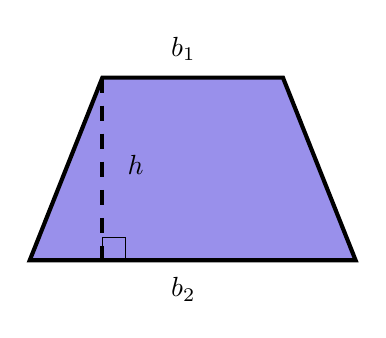
\begin{tikzpicture}[x=0.75pt,y=0.75pt,yscale=-1,xscale=1]
%uncomment if require: \path (0,153); %set diagram left start at 0, and has height of 153

%Shape: Trapezoid [id:dp6397225193899372] 
\draw  [fill={rgb, 255:red, 153; green, 144; blue, 235 }  ,fill opacity=1 ][line width=1.5]  (187,121) -- (222,33) -- (309,33) -- (344,121) -- cycle ;
%Straight Lines [id:da3353080959428809] 
\draw [line width=1.5]  [dash pattern={on 5.63pt off 4.5pt}]  (222,33) -- (222,121) ;


%Shape: Square [id:dp5126106092503966] 
\draw   (222,110) -- (233,110) -- (233,121) -- (222,121) -- cycle ;

% Text Node
\draw (261,19) node   {$b_{1}$};
% Text Node
\draw (261,135) node   {$b_{2}$};
% Text Node
\draw (238,75) node   {$h$};


\end{tikzpicture}
        \end{figure}
    \end{columns}
\end{frame}
%%%%%%%%%%%%%%%%%%%%%%%%%%%%%%%%%%%%%%%
%        SLIDE 
%%%%%%%%%%%%%%%%%%%%%%%%%%%%%%%%%%%%%%%
\begin{frame}[t]{Example (Find the Area)}
    \begin{example}
        Find the area of a below trapezoid.
        %
        \begin{figure}[H]
            \centering
            

\tikzset{every picture/.style={line width=0.75pt}} %set default line width to 0.75pt        

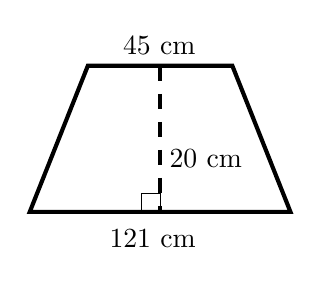
\begin{tikzpicture}[x=0.75pt,y=0.75pt,yscale=-1,xscale=1, scale=0.8]
%uncomment if require: \path (0,145); %set diagram left start at 0, and has height of 145

%Shape: Trapezoid [id:dp28634609077041273] 
\draw  [line width=1.5]  (243,109) -- (278,21) -- (365,21) -- (400,109) -- cycle ;
%Straight Lines [id:da16123629658218785] 
\draw [line width=1.5]  [dash pattern={on 5.63pt off 4.5pt}]  (321.5,21) -- (321.5,109) ;


%Shape: Square [id:dp7708997304192546] 
\draw   (310.5,98) -- (321.5,98) -- (321.5,109) -- (310.5,109) -- cycle ;

% Text Node
\draw (317,125) node   {$121\ \text{cm}$};
% Text Node
\draw (349,77) node   {$20\ \text{cm}$};
% Text Node
\draw (321,9) node   {$45\ \text{cm}$};


\end{tikzpicture}
        \end{figure}
    \end{example}
\end{frame}
%%%%%%%%%%%%%%%%%%%%%%%%%%%%%%%%%%%%%%%
%        SLIDE 
%%%%%%%%%%%%%%%%%%%%%%%%%%%%%%%%%%%%%%%
\section{More on Right Triangles}
\subsection{Pythagorean Theorem}
\begin{frame}[t]{Pythagorean Theorem}
    \begin{columns}[t]
    \column{0.45\textwidth}
        \begin{itemize}
            \item The Theorem of Pythagoras or Pythagorean theorem is a well-known theorem. 
            \item The theorem makes reference to a right triangle.
            \item As you might remember, The side opposite the right angle is the longest side and is called the hypotenuse.
        \end{itemize}
        %
    \column{0.45\textwidth}
        %
        \begin{block}{Formula}
            In a right triangle, the sum of the squares of the two right-angle sides (legs) will always be the same as the square of the hypotenuse. In symbol form:
            \[a^2+b^2 = c^2\]
        \end{block}
        %
        \begin{figure}[H]
            \centering
            \tikzset{every picture/.style={line width=0.75pt}} %set default line width to 0.75pt        
            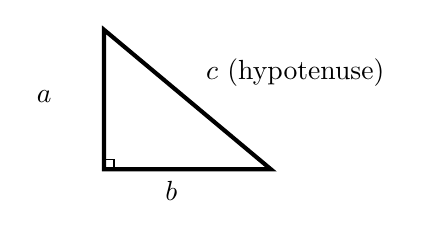
\begin{tikzpicture}[x=0.75pt,y=0.75pt,yscale=-1,xscale=1,scale=0.6]
            \draw  [line width=1.5]  (276,25) -- (410,137) -- (276,137) -- cycle ;
            \draw   (276,129) -- (284,129) -- (284,137) -- (276,137) -- cycle ;
            % Text Node
            \draw (228,79) node   {$a$};
            % Text Node
            \draw (330,154) node  {$b$};
            % Text Node
            \draw (350,59) node[right=0.1pt]   {$c\ \text{(hypotenuse)} \ $};
            \end{tikzpicture}
        \end{figure}
    \end{columns}
\end{frame}
%%%%%%%%%%%%%%%%%%%%%%%%%%%%%%%%%%%%%%%
%        SLIDE 
%%%%%%%%%%%%%%%%%%%%%%%%%%%%%%%%%%%%%%%
\begin{frame}[t]{Example (Find the missing side)}
    \begin{example}
        Find the missing side in each triangle.
        %
        \begin{figure}[H]
            \centering
            

\tikzset{every picture/.style={line width=0.75pt}} %set default line width to 0.75pt        

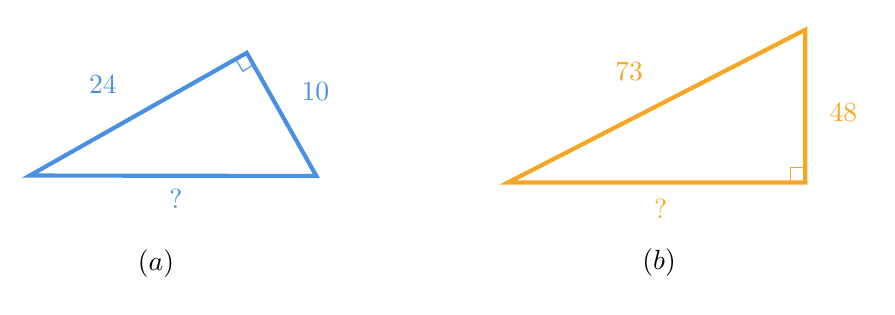
\begin{tikzpicture}[x=0.75pt,y=0.75pt,yscale=-1,xscale=1, scale=0.8]
%uncomment if require: \path (0,207); %set diagram left start at 0, and has height of 207

%Shape: Right Triangle [id:dp12946886895490128] 
\draw  [color={rgb, 255:red, 74; green, 144; blue, 226 }  ,draw opacity=1 ][line width=1.5]  (238.59,126.05) -- (65.98,125.8) -- (196.68,51.92) -- cycle ;
%Shape: Square [id:dp2641846486111634] 
\draw  [color={rgb, 255:red, 74; green, 144; blue, 226 }  ,draw opacity=1 ] (197,51.98) -- (201.19,58.8) -- (194.37,62.98) -- (190.18,56.17) -- cycle ;
%Shape: Right Triangle [id:dp9891393970753262] 
\draw  [color={rgb, 255:red, 245; green, 166; blue, 35 }  ,draw opacity=1 ][line width=1.5]  (533,38) -- (354,130) -- (533,130) -- cycle ;
%Shape: Square [id:dp34385770558966033] 
\draw  [color={rgb, 255:red, 245; green, 166; blue, 35 }  ,draw opacity=1 ] (524,121) -- (533,121) -- (533,130) -- (524,130) -- cycle ;

% Text Node
\draw (110,71) node   {$\textcolor[rgb]{0.29,0.56,0.89}{24}$};
% Text Node
\draw (238,75) node   {$\textcolor[rgb]{0.29,0.56,0.89}{10}$};
% Text Node
\draw (154,140) node   {$\textcolor[rgb]{0.29,0.56,0.89}{?}$};
% Text Node
\draw (427,63) node   {$\textcolor[rgb]{0.96,0.65,0.14}{73}$};
% Text Node
\draw (556,88) node   {$\textcolor[rgb]{0.96,0.65,0.14}{48}$};
% Text Node
\draw (446,146) node   {$\textcolor[rgb]{0.96,0.65,0.14}{?}$};
% Text Node
\draw (142,179) node   {$( a)$};
% Text Node
\draw (445,178) node   {$( b)$};


\end{tikzpicture}
        \end{figure}
    \end{example}   
\end{frame}
%%%%%%%%%%%%%%%%%%%%%%%%%%%%%%%%%%%%%%%
%        SLIDE 
%%%%%%%%%%%%%%%%%%%%%%%%%%%%%%%%%%%%%%%
\section{Circles}
\begin{frame}{Circles}
    \begin{itemize}
        \item A circle is a set of points that are the same distance from a fixed point.
        \item The fixed point is called center and we show it with letter $O$.
        \item A line segment from the center to a point on the circle is called radius denotes with $r$.
    \end{itemize}
    %
    \begin{figure}[H]
        \centering
        

\tikzset{every picture/.style={line width=0.75pt}} %set default line width to 0.75pt        

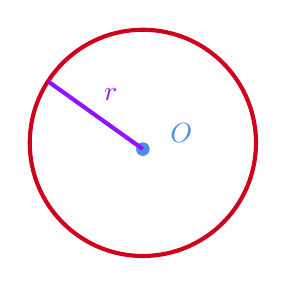
\begin{tikzpicture}[x=0.75pt,y=0.75pt,yscale=-1,xscale=1]
%uncomment if require: \path (0,140); %set diagram left start at 0, and has height of 140

%Shape: Circle [id:dp8118732481164563] 
\draw  [color={rgb, 255:red, 208; green, 2; blue, 27 }  ,draw opacity=1 ][line width=1.5]  (277,71.5) .. controls (277,41.4) and (301.4,17) .. (331.5,17) .. controls (361.6,17) and (386,41.4) .. (386,71.5) .. controls (386,101.6) and (361.6,126) .. (331.5,126) .. controls (301.4,126) and (277,101.6) .. (277,71.5) -- cycle ;
%Shape: Circle [id:dp14232976554180699] 
\draw  [color={rgb, 255:red, 74; green, 144; blue, 226 }  ,draw opacity=1 ][fill={rgb, 255:red, 74; green, 144; blue, 226 }  ,fill opacity=1 ] (328.5,74.5) .. controls (328.5,72.84) and (329.84,71.5) .. (331.5,71.5) .. controls (333.16,71.5) and (334.5,72.84) .. (334.5,74.5) .. controls (334.5,76.16) and (333.16,77.5) .. (331.5,77.5) .. controls (329.84,77.5) and (328.5,76.16) .. (328.5,74.5) -- cycle ;
%Straight Lines [id:da2079968527177969] 
\draw [color={rgb, 255:red, 144; green, 19; blue, 254 }  ,draw opacity=1 ][line width=1.5]    (286,42) -- (331.5,74.5) ;



% Text Node
\draw (350,67) node   {$\textcolor[rgb]{0.29,0.56,0.89}{O}$};
% Text Node
\draw (316,48) node   {$\textcolor[rgb]{0.56,0.07,1}{r}$};


\end{tikzpicture}
    \end{figure}
\end{frame}
%%%%%%%%%%%%%%%%%%%%%%%%%%%%%%%%%%%%%%%
%        SLIDE 
%%%%%%%%%%%%%%%%%%%%%%%%%%%%%%%%%%%%%%%
\begin{frame}{Circles (Cont'd)}
    \begin{itemize}
        \item The diameter, $d$, is a line segment passing though the center with endpoints on the circle.
        \[          r = \frac{d}{2}   \]
        \item Any other line segments with endpoints on the circle without passing though the center are called chords.
    \end{itemize}
    %
    \begin{figure}[H]
        \centering
        

\tikzset{every picture/.style={line width=0.75pt}} %set default line width to 0.75pt        

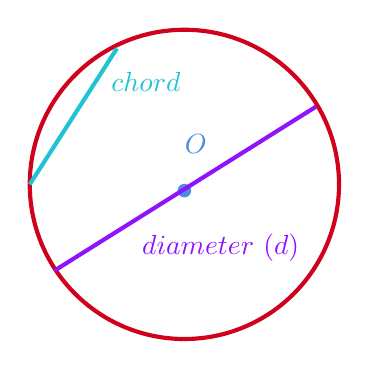
\begin{tikzpicture}[x=0.75pt,y=0.75pt,yscale=-1,xscale=1]
%uncomment if require: \path (0,188); %set diagram left start at 0, and has height of 188

%Shape: Circle [id:dp8118732481164563] 
\draw  [color={rgb, 255:red, 208; green, 2; blue, 27 }  ,draw opacity=1 ][line width=1.5]  (254,91.5) .. controls (254,50.35) and (287.35,17) .. (328.5,17) .. controls (369.65,17) and (403,50.35) .. (403,91.5) .. controls (403,132.65) and (369.65,166) .. (328.5,166) .. controls (287.35,166) and (254,132.65) .. (254,91.5) -- cycle ;
%Shape: Circle [id:dp14232976554180699] 
\draw  [color={rgb, 255:red, 74; green, 144; blue, 226 }  ,draw opacity=1 ][fill={rgb, 255:red, 74; green, 144; blue, 226 }  ,fill opacity=1 ] (325.83,93.13) .. controls (326.58,91.66) and (328.39,91.07) .. (329.87,91.83) .. controls (331.34,92.58) and (331.93,94.39) .. (331.17,95.87) .. controls (330.42,97.34) and (328.61,97.93) .. (327.13,97.17) .. controls (325.66,96.42) and (325.07,94.61) .. (325.83,93.13) -- cycle ;
%Straight Lines [id:da2079968527177969] 
\draw [color={rgb, 255:red, 144; green, 19; blue, 254 }  ,draw opacity=1 ][line width=1.5]    (266,133) -- (392,54) ;


%Straight Lines [id:da9513159212046638] 
\draw [color={rgb, 255:red, 33; green, 195; blue, 211 }  ,draw opacity=1 ][line width=1.5]    (296,26) -- (254,91.5) ;



% Text Node
\draw (334,72) node   {$\textcolor[rgb]{0.29,0.56,0.89}{O}$};
% Text Node
\draw (346,122) node   {$\textcolor[rgb]{0.56,0.07,1}{diameter\ ( d)}$};
% Text Node
\draw (310,42) node [color={rgb, 255:red, 33; green, 195; blue, 211 }  ,opacity=1 ]  {$\textcolor[rgb]{0.13,0.76,0.83}{chord}$};


\end{tikzpicture}
    \end{figure}
\end{frame}
%%%%%%%%%%%%%%%%%%%%%%%%%%%%%%%%%%%%%%%
%        SLIDE 
%%%%%%%%%%%%%%%%%%%%%%%%%%%%%%%%%%%%%%%
\subsection{Number \texorpdfstring{$\pi$}{TEXT} }
\begin{frame}{Number $\pi$}
    %
    \begin{itemize}
        \item \textit{Archimedes} was a Greek mathematician, physicist, engineer, and astronomer.
        \item He discovered that in any circle the ratio of circumference to diameter is always the same number $3.14159\cdots$
        \item It has been represented by the Greek letter $\pi$ since the mid-18th century, though it is also sometimes spelled out as ``pi''.
    \end{itemize}
    %
    \begin{figure}[H]
        \centering
        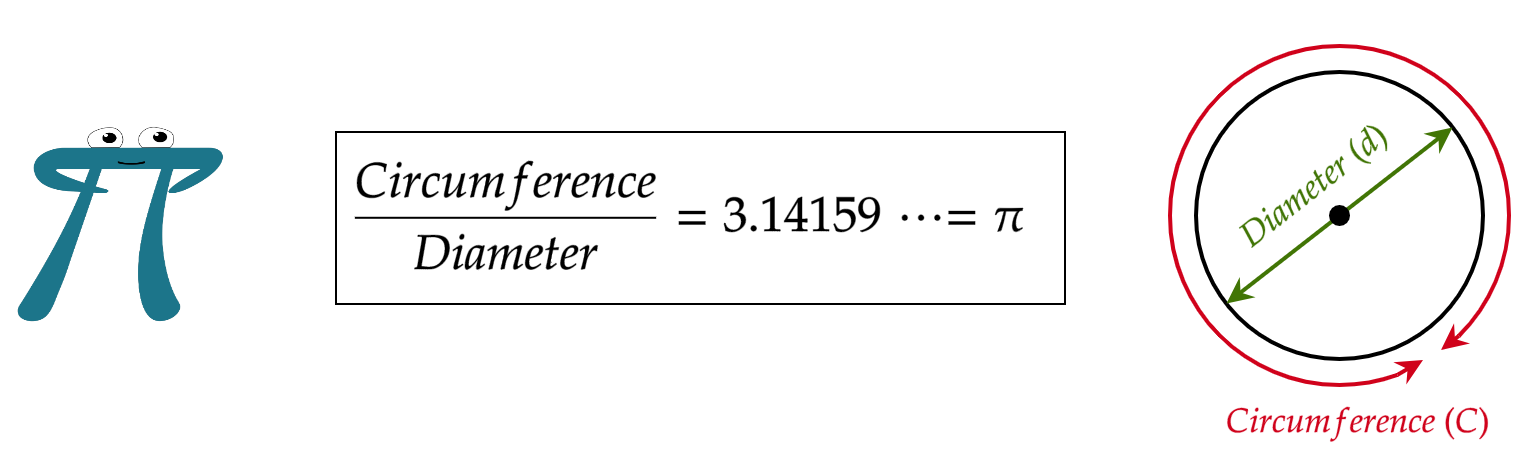
\includegraphics[scale=0.27]{pics/circumference_to_diameter.png}
    \end{figure}
\end{frame}
%%%%%%%%%%%%%%%%%%%%%%%%%%%%%%%%%%%%%%%
%        SLIDE 
%%%%%%%%%%%%%%%%%%%%%%%%%%%%%%%%%%%%%%%
\begin{frame}{Number $\pi$ (Cont'd)}
    \begin{columns}
    \column{0.45\textwidth}
    \begin{itemize}
        \item $\pi$ is a constant number.
        \item It is a irrational number since we cannot express it as a fraction.
        \item But its digits goes forever.
        \item In most cases, we leave our answers in terms of $\pi$ unless the problem itself give us some approximation.
    \end{itemize}
    %
    \column{0.45\textwidth}
    \begin{figure}[H]
        \centering
        
\includegraphics[scale=0.3]{pics/pi_funny.jpg}
    \end{figure}
    \end{columns}
\end{frame}
%%%%%%%%%%%%%%%%%%%%%%%%%%%%%%%%%%%%%%%
%        SLIDE 
%%%%%%%%%%%%%%%%%%%%%%%%%%%%%%%%%%%%%%%
\subsection{Circumference of a Circle}
\begin{frame}[t]{Circumference of a Circle}
    \begin{itemize}
        \item Circumference is denoted as $C$.
        \item We learned circumference divided by diameter is always equal to $\pi$.
        \item If we multiply both sides of the equation by $2r$, we will get an equation for $C$.
    \end{itemize}
    %
    \begin{columns}[t]
    \column{0.45\textwidth}
    \begin{block}{Circumference of a Circle}
        The circumference of a circle, $C$, with radius $r$ is
        \[ C = 2\pi r\]
    \end{block}
    %
    \column{0.45\textwidth}
    \begin{figure}[H]
        \centering
        
\includegraphics[scale=0.13]{pics/wow.jpg}
    \end{figure}
    \end{columns}
\end{frame}
%%%%%%%%%%%%%%%%%%%%%%%%%%%%%%%%%%%%%%%
%        SLIDE 
%%%%%%%%%%%%%%%%%%%%%%%%%%%%%%%%%%%%%%%
\subsection{Area of a Circle}
\begin{frame}[t]{Area of a Circle}
    %
    \begin{columns}
    \column{0.45\textwidth}
    \begin{itemize}
            \item \textit{Archimedes} also found the area of the circle by dividing circles into some sectors. 
            \item He then argued the area of those slices is the same as a right triangle whose is $2\pi r$ and its height $r$.
        \end{itemize}
    %
    \column{0.45\textwidth}
    \begin{block}{Area of a Circle}
        The area of a circle with radius $r$ is
        \[ A = \pi r^2\]
    \end{block}
    %
    \end{columns}
    %
    \begin{figure}
        \centering
        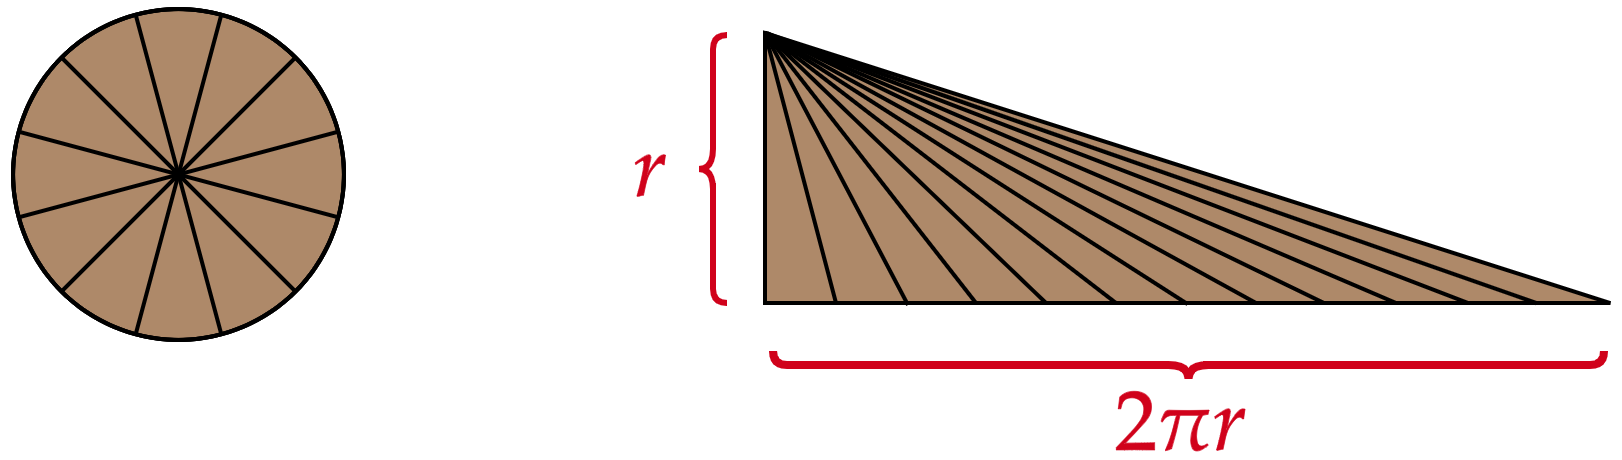
\includegraphics[scale=0.23]{pics/archimede_area.png}
    \end{figure}
\end{frame}
%%%%%%%%%%%%%%%%%%%%%%%%%%%%%%%%%%%%%%%
%        SLIDE 
%%%%%%%%%%%%%%%%%%%%%%%%%%%%%%%%%%%%%%%
\begin{frame}[t]{Example (Find Circumference and Area)}
    \begin{example}
        Find the circumference and area of a circle with diameter 12 cm.
    \end{example}
\end{frame}
% PART 4 (SECTION 8.4)
\part{Section 8.4}
%%%%%%%%%%%%%%%%%%%%%%%%%%%%%%%%%%%%%%%
\begin{transitionframe}
    \begin{center}
    { 
        \Huge \textcolor{white}{\textbf{Volume and Surface Area}}
        \\[-1em]
        \noindent\textcolor{white}{\rule{12cm}{0.4pt}}
        
        %\large \textcolor{white}{Section 8.4}
    }
    \end{center}
\end{transitionframe}
%%%%%%%%%%%%%%%%%%%%%%%%%%%%%%%%%%%%%%%
%        SLIDE 
%%%%%%%%%%%%%%%%%%%%%%%%%%%%%%%%%%%%%%%
\begin{frame}{Outline}
    \begin{columns}[t]
        \begin{column}{.5\textwidth}
            \tableofcontents[part=4, sections={1-2}]
        \end{column}
        \begin{column}{.5\textwidth}
            \tableofcontents[part=4, sections={3-4}]
        \end{column}
    \end{columns}
\end{frame}
%%%%%%%%%%%%%%%%%%%%%%%%%%%%%%%%%%%%%%%
%        SLIDE 
%%%%%%%%%%%%%%%%%%%%%%%%%%%%%%%%%%%%%%%
\section{Polyhedra}
\subsection{What is Polyhedra?}
\begin{frame}{Polyhedra}
    \begin{itemize}
        \item A polyhedron (plural polyhedra) is closed figure formed by a number of polygons.
    \end{itemize}
    %
    \begin{block}{Definition}
        A polyhedron must meet 3 conditions:
        \begin{itemize}
            \item closed figure
            \item created by straight lines only
            \item 3-Dimensional object
        \end{itemize}
    \end{block}
    %
    \begin{figure}[H]
        \centering
        % DEFINING COLORS COF, PUR, GREEO AND GREET
\definecolor{cof}{RGB}{219,144,71}
\definecolor{pur}{RGB}{186,146,162}
\definecolor{greeo}{RGB}{91,173,69}
\definecolor{greet}{RGB}{52,111,72}
% TETRAHEDRON
\begin{tikzpicture}[thick,scale=2.5]
    \coordinate (A1) at (0,0);
    \coordinate (A2) at (0.6,0.2);
    \coordinate (A3) at (1,0);
    \coordinate (A4) at (0.4,-0.2);
    \coordinate (B1) at (0.5,0.5);
    %
    \begin{scope}[thick,dashed,,opacity=0.6]
        \draw (A1) -- (A2) -- (A3);
        \draw (B1) -- (A2);
    \end{scope}
    \draw[fill=cof,opacity=0.6] (A1) -- (A4) -- (B1);
    \draw[fill=pur,opacity=0.6] (A4) -- (B1) -- (A3);
    %
    \draw (A1) -- (B1) -- (A4) --cycle;
    \draw (A4) -- (A3) -- (B1) ;
    %
\end{tikzpicture}
% RECTANGULAR CUBE
\begin{tikzpicture}[thick,scale=2.5]
    \coordinate (A1) at (0,0);
    \coordinate (A2) at (0.6,0.2);
    \coordinate (A3) at (1,0);
    \coordinate (A4) at (0.4,-0.2);
    \coordinate (B1) at (0,0.5);
    \coordinate (B2) at (0.6,0.7);
    \coordinate (B3) at (1,0.5);
    \coordinate (B4) at (0.4,0.3);
    %
    \begin{scope}[thick,dashed,,opacity=0.6]
        \draw (A1) -- (A2) -- (A3);
        \draw (A2) -- (B2);
    \end{scope}
    %
    \draw[fill=cof,opacity=0.6] (A1) -- (B1) -- (B4) -- (A4);
    \draw[fill=pur,opacity=0.6] (A4) -- (B4) -- (B3) -- (A3);
    \draw[fill=greeo,opacity=0.6] (B4) -- (B1) -- (B2) -- (B3);
    %
    \draw (A1) -- (B1) -- (B4) -- (A4) --cycle;
    \draw (A4) -- (B4) -- (B3) -- (A3) --cycle;
    \draw (B4) -- (B1) -- (B2) -- (B3) --cycle;
    %
\end{tikzpicture}
% OCTAHEDRON
\begin{tikzpicture}[thick,scale=2.5]
    \coordinate (A1) at (0,0);
    \coordinate (A2) at (0.6,0.2);
    \coordinate (A3) at (1,0);
    \coordinate (A4) at (0.4,-0.2);
    \coordinate (B1) at (0.5,0.5);
    \coordinate (B2) at (0.5,-0.5);
    %
    \begin{scope}[thick,dashed,,opacity=0.6]
        \draw (A1) -- (A2) -- (A3);
        \draw (B1) -- (A2) -- (B2);
    \end{scope}
    %
    \draw[fill=cof,opacity=0.6] (A1) -- (A4) -- (B1);
    \draw[fill=pur,opacity=0.6] (A1) -- (A4) -- (B2);
    \draw[fill=greeo,opacity=0.6] (A3) -- (A4) -- (B1);
    \draw[fill=greet,opacity=0.6] (A3) -- (A4) -- (B2);
    \draw (B1) -- (A1) -- (B2) -- (A3) --cycle;
\end{tikzpicture}
% Prism
\begin{tikzpicture}[thick,scale=2.5]
    \coordinate (A1) at (0,0);
    \coordinate (A3) at (0.7,0);
    \coordinate (A4) at (0,-0.75);
    \coordinate (A5) at (0.7,-0.75);
    \coordinate (B1) at (0.35,0.3);
    \coordinate (B2) at (0.35,-0.5);
    %
    \begin{scope}[thick,dashed,opacity=0.6]
        \draw (B1)  -- (B2);
        \draw (A4) -- (B2);
        \draw (A5) -- (B2);
    \end{scope}
    %
    \draw[fill=cof,opacity=0.6] (A1) -- (B1) -- (A3);
    \draw[fill=pur,opacity=0.6] (A1) -- (A3) -- (A5) -- (A4);
    %
    \draw (A1) -- (B1) -- (A3) -- (A5) -- (A4) --cycle;
    %
\end{tikzpicture}
    \end{figure}
\end{frame}
%%%%%%%%%%%%%%%%%%%%%%%%%%%%%%%%%%%%%%%
%        SLIDE 
%%%%%%%%%%%%%%%%%%%%%%%%%%%%%%%%%%%%%%%
\subsection{Faces, Vertices, and Edges}
\begin{frame}{Faces, Vertices, and Edges}
    \begin{itemize}
        \item \textbf{Face}: Each flat surface (or each polygon).
        \item \textbf{Vertex}: Corners of faces.
        \item \textbf{Edge}: A line segment between two faces.
    \end{itemize}
    %
    \begin{figure}[H]
        \centering
        

\tikzset{every picture/.style={line width=0.75pt}} %set default line width to 0.75pt        

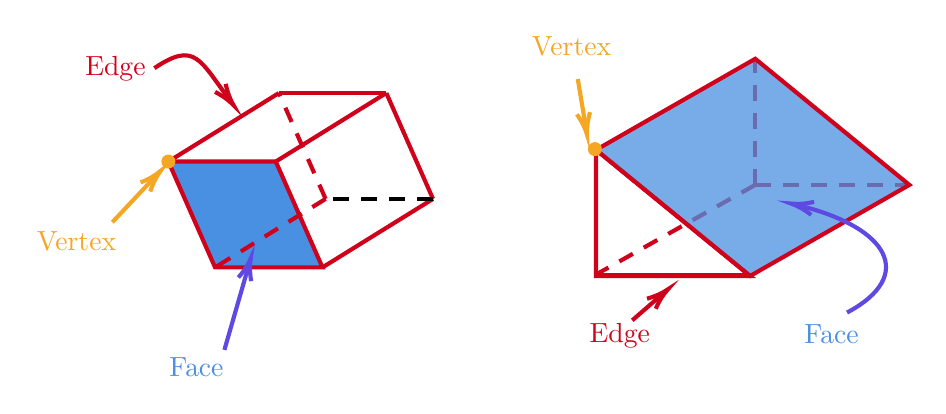
\begin{tikzpicture}[x=0.75pt,y=0.75pt,yscale=-1,xscale=1, scale= 0.75]
%uncomment if require: \path (0,288); %set diagram left start at 0, and has height of 288

%Shape: Rectangle [id:dp053370527561274805] 
\draw  [color={rgb, 255:red, 208; green, 2; blue, 27 }  ,draw opacity=1 ][fill={rgb, 255:red, 74; green, 144; blue, 226 }  ,fill opacity=1 ][line width=1.5]  (130,96) -- (199,96) -- (229,164) -- (160,164) -- cycle ;
%Straight Lines [id:da7233344038492684] 
\draw [color={rgb, 255:red, 208; green, 2; blue, 27 }  ,draw opacity=1 ][line width=1.5]    (199,96) -- (270,52) ;


%Straight Lines [id:da8870385695360932] 
\draw [color={rgb, 255:red, 208; green, 2; blue, 27 }  ,draw opacity=1 ][line width=1.5]    (130,96) -- (201,52) ;


%Straight Lines [id:da6880167264201218] 
\draw [color={rgb, 255:red, 208; green, 2; blue, 27 }  ,draw opacity=1 ][line width=1.5]    (229,164) -- (300,120) ;


%Straight Lines [id:da8629284451428976] 
\draw [color={rgb, 255:red, 208; green, 2; blue, 27 }  ,draw opacity=1 ][line width=1.5]    (300,120) -- (270,52) ;


%Straight Lines [id:da5801797655392487] 
\draw [color={rgb, 255:red, 208; green, 2; blue, 27 }  ,draw opacity=1 ][line width=1.5]    (270,52) -- (201,52) ;


%Straight Lines [id:da33437733704095596] 
\draw [color={rgb, 255:red, 208; green, 2; blue, 27 }  ,draw opacity=1 ][line width=1.5]  [dash pattern={on 5.63pt off 4.5pt}]  (231,120) -- (201,52) ;


%Straight Lines [id:da7324938230911522] 
\draw [line width=1.5]  [dash pattern={on 5.63pt off 4.5pt}]  (300,120) -- (231,120) ;


%Straight Lines [id:da04595951918657737] 
\draw [color={rgb, 255:red, 208; green, 2; blue, 27 }  ,draw opacity=1 ][line width=1.5]  [dash pattern={on 5.63pt off 4.5pt}]  (231,120) -- (160,164) ;


%Shape: Right Triangle [id:dp15828119672901897] 
\draw  [color={rgb, 255:red, 208; green, 2; blue, 27 }  ,draw opacity=1 ][line width=1.5]  (404.75,88.5) -- (503.75,169.5) -- (404.75,169.5) -- cycle ;
%Straight Lines [id:da18371357143649392] 
\draw [color={rgb, 255:red, 208; green, 2; blue, 27 }  ,draw opacity=1 ][line width=1.5]  [dash pattern={on 5.63pt off 4.5pt}]  (507,111) -- (507,30) ;


%Straight Lines [id:da5323303129683379] 
\draw [color={rgb, 255:red, 208; green, 2; blue, 27 }  ,draw opacity=1 ][line width=1.5]  [dash pattern={on 5.63pt off 4.5pt}]  (507,111) -- (606,111) ;


%Straight Lines [id:da1934412072495324] 
\draw [color={rgb, 255:red, 208; green, 2; blue, 27 }  ,draw opacity=1 ][line width=1.5]  [dash pattern={on 5.63pt off 4.5pt}]  (404,169) -- (507,111) ;


%Curve Lines [id:da9915257466456324] 
\draw [color={rgb, 255:red, 208; green, 2; blue, 27 }  ,draw opacity=1 ][line width=1.5]    (121,36) .. controls (147.33,18.45) and (149.88,30.37) .. (170.39,57.86) ;
\draw [shift={(172,60)}, rotate = 232.82] [color={rgb, 255:red, 208; green, 2; blue, 27 }  ,draw opacity=1 ][line width=1.5]    (14.21,-4.28) .. controls (9.04,-1.82) and (4.3,-0.39) .. (0,0) .. controls (4.3,0.39) and (9.04,1.82) .. (14.21,4.28)   ;

%Shape: Circle [id:dp6348766282723517] 
\draw  [draw opacity=0][fill={rgb, 255:red, 245; green, 166; blue, 35 }  ,fill opacity=1 ] (125.5,96) .. controls (125.5,93.51) and (127.51,91.5) .. (130,91.5) .. controls (132.49,91.5) and (134.5,93.51) .. (134.5,96) .. controls (134.5,98.49) and (132.49,100.5) .. (130,100.5) .. controls (127.51,100.5) and (125.5,98.49) .. (125.5,96) -- cycle ;
%Straight Lines [id:da9603817642462407] 
\draw [color={rgb, 255:red, 245; green, 166; blue, 35 }  ,draw opacity=1 ][line width=1.5]    (94,135) -- (122.95,104.19) ;
\draw [shift={(125,102)}, rotate = 493.21] [color={rgb, 255:red, 245; green, 166; blue, 35 }  ,draw opacity=1 ][line width=1.5]    (14.21,-4.28) .. controls (9.04,-1.82) and (4.3,-0.39) .. (0,0) .. controls (4.3,0.39) and (9.04,1.82) .. (14.21,4.28)   ;

%Straight Lines [id:da6450171763852104] 
\draw [color={rgb, 255:red, 94; green, 74; blue, 226 }  ,draw opacity=1 ][line width=1.5]    (166,217) -- (182.17,160.88) ;
\draw [shift={(183,158)}, rotate = 466.07] [color={rgb, 255:red, 94; green, 74; blue, 226 }  ,draw opacity=1 ][line width=1.5]    (14.21,-4.28) .. controls (9.04,-1.82) and (4.3,-0.39) .. (0,0) .. controls (4.3,0.39) and (9.04,1.82) .. (14.21,4.28)   ;

%Shape: Polygon [id:ds14971897219625419] 
\draw  [color={rgb, 255:red, 208; green, 2; blue, 27 }  ,draw opacity=1 ][fill={rgb, 255:red, 74; green, 144; blue, 226 }  ,fill opacity=0.75 ][line width=1.5]  (507,30) -- (606,111) -- (503.75,169.5) -- (404.75,88.5) -- cycle ;
%Straight Lines [id:da1871099492645416] 
\draw [color={rgb, 255:red, 208; green, 2; blue, 27 }  ,draw opacity=1 ][line width=1.5]    (503,169) -- (404,169) ;


%Straight Lines [id:da5598317572787015] 
\draw [color={rgb, 255:red, 208; green, 2; blue, 27 }  ,draw opacity=1 ][line width=1.5]    (428,198) -- (448.74,179.97) ;
\draw [shift={(451,178)}, rotate = 498.99] [color={rgb, 255:red, 208; green, 2; blue, 27 }  ,draw opacity=1 ][line width=1.5]    (14.21,-4.28) .. controls (9.04,-1.82) and (4.3,-0.39) .. (0,0) .. controls (4.3,0.39) and (9.04,1.82) .. (14.21,4.28)   ;

%Shape: Circle [id:dp5936650276871587] 
\draw  [draw opacity=0][fill={rgb, 255:red, 245; green, 166; blue, 35 }  ,fill opacity=1 ] (399.5,88) .. controls (399.5,85.51) and (401.51,83.5) .. (404,83.5) .. controls (406.49,83.5) and (408.5,85.51) .. (408.5,88) .. controls (408.5,90.49) and (406.49,92.5) .. (404,92.5) .. controls (401.51,92.5) and (399.5,90.49) .. (399.5,88) -- cycle ;
%Straight Lines [id:da46178057371883363] 
\draw [color={rgb, 255:red, 245; green, 166; blue, 35 }  ,draw opacity=1 ][line width=1.5]    (393,43) -- (398.51,76.04) ;
\draw [shift={(399,79)}, rotate = 260.54] [color={rgb, 255:red, 245; green, 166; blue, 35 }  ,draw opacity=1 ][line width=1.5]    (14.21,-4.28) .. controls (9.04,-1.82) and (4.3,-0.39) .. (0,0) .. controls (4.3,0.39) and (9.04,1.82) .. (14.21,4.28)   ;

%Curve Lines [id:da39173533566192775] 
\draw [color={rgb, 255:red, 94; green, 74; blue, 226 }  ,draw opacity=1 ][line width=1.5]    (566,193) .. controls (610.33,169.36) and (593.53,137.96) .. (532.8,123.64) ;
\draw [shift={(530,123)}, rotate = 372.53] [color={rgb, 255:red, 94; green, 74; blue, 226 }  ,draw opacity=1 ][line width=1.5]    (14.21,-4.28) .. controls (9.04,-1.82) and (4.3,-0.39) .. (0,0) .. controls (4.3,0.39) and (9.04,1.82) .. (14.21,4.28)   ;


% Text Node
\draw (96,36) node  [align=left] {\textcolor[rgb]{0.82,0.01,0.11}{Edge}};
% Text Node
\draw (71,147) node  [align=left] {\textcolor[rgb]{0.96,0.65,0.14}{Vertex}};
% Text Node
\draw (148,228) node [color={rgb, 255:red, 74; green, 144; blue, 226 }  ,opacity=1 ] [align=left] {\textcolor[rgb]{0.29,0.56,0.89}{Face}};
% Text Node
\draw (420,208) node  [align=left] {\textcolor[rgb]{0.82,0.01,0.11}{Edge}};
% Text Node
\draw (556,207) node [color={rgb, 255:red, 74; green, 144; blue, 226 }  ,opacity=1 ] [align=left] {\textcolor[rgb]{0.29,0.56,0.89}{Face}};
% Text Node
\draw (389,22) node  [align=left] {\textcolor[rgb]{0.96,0.65,0.14}{Vertex}};
% % Text Node
% \draw (198,268) node   {$( a)$};
% % Text Node
% \draw (485,268) node   {$( b)$};


\end{tikzpicture}
    \end{figure}
\end{frame}
%%%%%%%%%%%%%%%%%%%%%%%%%%%%%%%%%%%%%%%
%        SLIDE 
%%%%%%%%%%%%%%%%%%%%%%%%%%%%%%%%%%%%%%%
\subsection{Euler's Polyhedron Formula}
\begin{frame}[t]{Euler's Polyhedron Formula}
    \begin{columns}[c]
        \column{0.45\textwidth}
        %
        \begin{itemize}
            \item Leonhard Euler was a Swiss mathematician who made enormous contributions to a wide range of fields in mathematics.
            \item Euler discovered a relation between number of vertices, number of faces, and number of edges.
        \end{itemize}
        %
        \begin{block}{Euler's Formula}
             Let $V$ be the number of vertices, $E$ be the number of edges and $F$ be the number of faces of a polyhedon. Then
             \[ V-E+F=2 \]
        \end{block}
        %***** 2nd column *****
        \column{0.45\textwidth}    
        %
        \begin{figure}[H]
            \centering
            \includegraphics[width=0.6\textwidth]{pics/Leonhard_Euler.jpg}
            \caption*{Leonhard Euler (1707-1783)}
        \end{figure}
        % \begin{figure}[H]
        %     \centering
        %     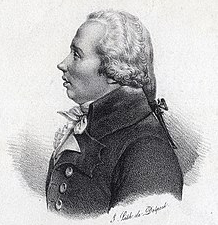
\includegraphics[width=0.35\textwidth]{pics/legendre.png}
        % \end{figure}
        % \begin{itemize}
        %     \item Euler mentioned his result in a letter to Goldbach in 1750. However he did not give the first correct proof of his formula.
        %     \item French mathematician Adrian Marie Legendre (1752-1833) was the first to prove using Spherical Geometry.
        % \end{itemize}
    \end{columns}

\end{frame}
%%%%%%%%%%%%%%%%%%%%%%%%%%%%%%%%%%%%%%%
%        SLIDE 
%%%%%%%%%%%%%%%%%%%%%%%%%%%%%%%%%%%%%%%
\begin{frame}{Euler's Polyhedron Formula (Cont'd)}
    \textbf{Examples}:
    %
    \begin{columns}
    %
    \column{0.25\textwidth}
    \begin{figure}[H]
        \centering
        % DEFINING COLORS COF, PUR, GREEO AND GREET
\definecolor{cof}{RGB}{219,144,71}
\definecolor{pur}{RGB}{186,146,162}
\definecolor{greeo}{RGB}{91,173,69}
\definecolor{greet}{RGB}{52,111,72}
% CUBE
\begin{tikzpicture}[thick,scale=0.8,DarkSlateGray]
    \coordinate (A1) at (-1,-1,-1);
    \coordinate (A2) at (-1,-1,1);
    \coordinate (A3) at (-1,1,-1);
    \coordinate (A4) at (-1,1,1);
    \coordinate (B1) at (1,-1,-1);
    \coordinate (B2) at (1,-1,1);
    \coordinate (B3) at (1,1,-1);
    \coordinate (B4) at (1,1,1);
    %
    % Drawing dashed lines
    \begin{scope}[thick,dashed,opacity=0.6]
        \draw (A2) -- (A1) -- (B1);
        \draw (A1) -- (A3);
    \end{scope}
    %
    % Color Faces
    \draw[fill=cof,opacity=0.6]   (A4) -- (B4) -- (B2) -- (A2) ;
    \draw[fill=greet,opacity=0.6]   (B4) -- (B3) -- (B1) -- (B2) ;
    \draw[fill=greeo,opacity=0.6] (A4) -- (B4) -- (B3) -- (A3) ;
    %
    % Drawing Edges
    \draw (A2) -- (B2) -- (B1) ;
    \draw (A2) -- (A4) -- (B4) -- (B2) -- cycle ;
    \draw (A4) -- (A3) -- (B3) -- (B4) ;   
    \draw (B3) -- (B1);
    %
\end{tikzpicture}
    \end{figure}
    %
    \begin{center}
        Cube
    \end{center}
    %
    \begin{align*}
        & V=8,\; E=12,\; F=6
        \\
        &V-E+F = 2\ \checkmark
    \end{align*}   
    %
    \column{0.33\textwidth}
    \begin{figure}[H]
        \centering
        % DEFINING COLORS COF, PUR, GREEO AND GREET
\definecolor{cof}{RGB}{219,144,71}
\definecolor{pur}{RGB}{186,146,162}
\definecolor{greeo}{RGB}{91,173,69}
\definecolor{greet}{RGB}{52,111,72}
% Icosphedron
    \tdplotsetmaincoords{60}{100}
    \begin{tikzpicture}[tdplot_main_coords,scale=1,line join=round, scale=0.4]
    \pgfmathsetmacro\a{2}
    \pgfmathsetmacro{\phi}{\a*(1+sqrt(5))/2}
    \path 
    coordinate(A) at (0,\phi,\a)
    coordinate(B) at (0,\phi,-\a)
    coordinate(C) at (0,-\phi,\a)
    coordinate(D) at (0,-\phi,-\a)
    coordinate(E) at (\a,0,\phi)
    coordinate(F) at (\a,0,-\phi)
    coordinate(G) at (-\a,0,\phi)
    coordinate(H) at (-\a,0,-\phi)
    coordinate(I) at (\phi,\a,0)
    coordinate(J) at (\phi,-\a,0)
    coordinate(K) at (-\phi,\a,0)
    coordinate(L) at (-\phi,-\a,0); 
    \draw[dashed, thick]    (B) -- (H) -- (F) 
    (D) -- (L) -- (H) --cycle 
    (K) -- (L) -- (H) --cycle
    (K) -- (L) -- (G) --cycle
    (C) -- (L) (B)--(K) (A)--(K)
    ;

        \draw[thick]
        (A) -- (I) -- (B) --cycle 
        (F) -- (I) -- (B) --cycle 
        (F) -- (I) -- (J) --cycle
        (F) -- (D) -- (J) --cycle
        (C) -- (D) -- (J) --cycle
        (C) -- (E) -- (J) --cycle
        (I) -- (E) -- (J) --cycle
        (I) -- (E) -- (A) --cycle
        (G) -- (E) -- (A) --cycle
        (G) -- (E) -- (C) --cycle
        ; 
        \draw[fill=DarkSeaGreen,opacity=0.6] (A) -- (I) -- (B) --cycle ;
        \draw[fill=DarkKhaki,opacity=0.6]  (F) -- (I) -- (B) --cycle ;
        \draw[fill=Tan,opacity=0.6]  (F) -- (I) -- (J) --cycle;
        \draw[fill=CadetBlue,opacity=0.6]  (F) -- (D) -- (J) --cycle;
        \draw[fill=LightYellow,opacity=0.6]    (C) -- (D) -- (J) --cycle;
        \draw[fill=Thistle,opacity=0.6]   (C) -- (E) -- (J) --cycle;
        \draw[fill=DarkGray,opacity=0.6]  (I) -- (E) -- (J) --cycle;
        \draw[fill=LightSteelBlue,opacity=0.6]     (I) -- (E) -- (A) --cycle;
        \draw[fill=DarkSalmon,opacity=0.6]   (G) -- (E) -- (A) --cycle;
        \draw[fill=LightPink,opacity=0.6]    (G) -- (E) -- (C) --cycle;
\end{tikzpicture}
    \end{figure}   
    %
    \begin{center}
        Icosahedron 
    \end{center}
    %
    %
    \begin{align*}
        & V=12,\; E=30,\; F=20
        \\
        &V-E+F = 2\ \checkmark
    \end{align*}   
    %
    \end{columns}
\end{frame}
%%%%%%%%%%%%%%%%%%%%%%%%%%%%%%%%%%%%%%%
%        SLIDE 
%%%%%%%%%%%%%%%%%%%%%%%%%%%%%%%%%%%%%%%
\begin{frame}[t]{Example (Does this shape exist?)}
    \begin{example}
        Do the following shapes exist?
        \begin{enumerate}[(a)]
            \item A polyhedron with $V=10$, $E=22$, and $F=14$
            \item A polyhedron with $V= 14$, $E=21$, and $F= 10$
        \end{enumerate}
    \end{example}
\end{frame}
%%%%%%%%%%%%%%%%%%%%%%%%%%%%%%%%%%%%%%%
%        SLIDE 
%%%%%%%%%%%%%%%%%%%%%%%%%%%%%%%%%%%%%%%
\begin{frame}[t]{Example (Euler's Formula)}
    \begin{example}
        A certain polyhedron has 16 vertices and 10 faces. Determine the number of edges on the polyhedron.
    \end{example}
\end{frame}
%%%%%%%%%%%%%%%%%%%%%%%%%%%%%%%%%%%%%%%
%        SLIDE 
%%%%%%%%%%%%%%%%%%%%%%%%%%%%%%%%%%%%%%%
\section{Types of Polyhedra}
\begin{frame}[t]{Types of Polyhedra}
    \begin{figure}[h]
        \centering
        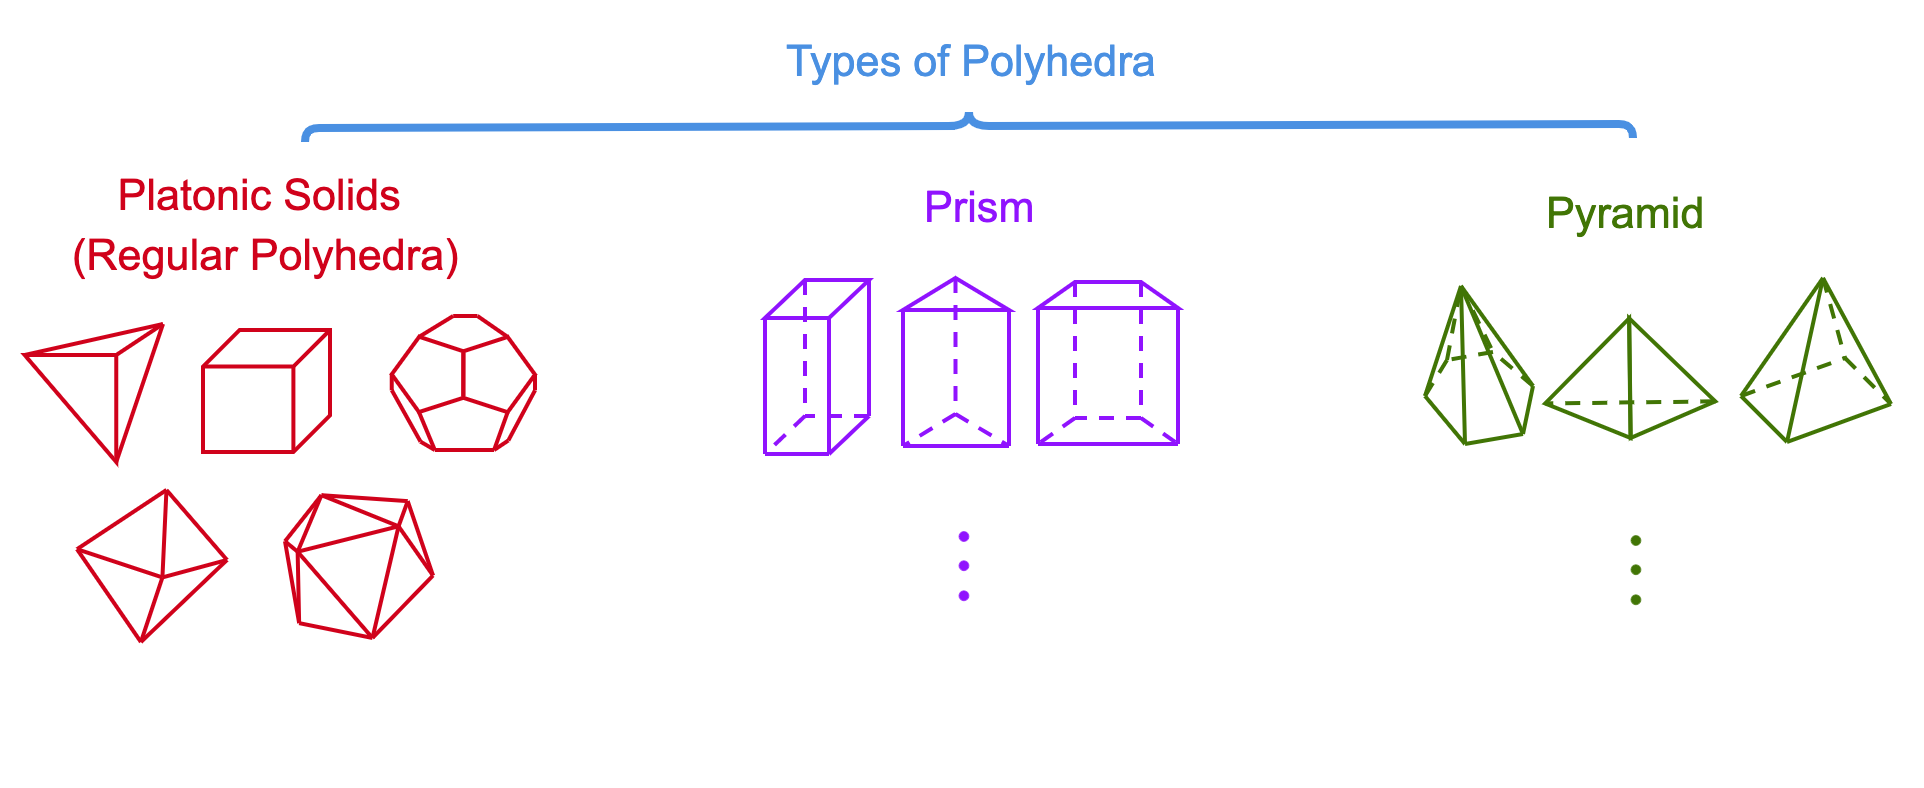
\includegraphics[scale=0.22]{pics/types_polyhedra.png}
    \end{figure}
\end{frame}
%%%%%%%%%%%%%%%%%%%%%%%%%%%%%%%%%%%%%%%
%        SLIDE 
%%%%%%%%%%%%%%%%%%%%%%%%%%%%%%%%%%%%%%%
\subsection{Platonic Solids}
\begin{frame}[t]{Platonic Solids}
    %
    \begin{itemize}
        \item All faces are \textbf{regular} polygons of the same size and shape.
        \item There are only 5 platonic solids (why? watch this video from \hyperlink{http://www.youtube.com/watch?v=gVzu1_12FUc}{\textcolor{blue}{\underline{Numberphile}}}).
    \end{itemize}
    %
    \begin{figure}[H]
        \centering
        % DEFINING COLORS COF, PUR, GREEO AND GREET
\definecolor{cof}{RGB}{219,144,71}
\definecolor{pur}{RGB}{186,146,162}
\definecolor{greeo}{RGB}{91,173,69}
\definecolor{greet}{RGB}{52,111,72}

% Tetrahedron
\tdplotsetmaincoords{70}{100} 
\begin{tikzpicture}[thick, line join=round,tdplot_main_coords,declare function={a=5;},scale=0.5,DarkSlateGray] 
    \begin{scope}[canvas is xy plane at z=0,transform shape]
         \path[thick] foreach \X [count=\Y] in {A,B,C}
         {(\Y*120:{a/(2*cos(30))}) coordinate(\X)};
    \end{scope}
    %
    \path[thick] (0,0,{a*cos(30)}) coordinate (D);
    %
    \draw[dashed,opacity=0.6] (A) -- (B);
     %
    \draw[fill=greeo,opacity=0.6] (D) -- (B) -- (C) --cycle ;
    \draw[fill=cof,opacity=0.6]  (A) -- (C) -- (D) --cycle ;
    
    \node[thick,below=0.5cm] {Tetrahedron};
\end{tikzpicture}
% CUBE
\begin{tikzpicture}[thick,scale=0.8,DarkSlateGray]
    \coordinate (A1) at (-1,-1,-1);
    \coordinate (A2) at (-1,-1,1);
    \coordinate (A3) at (-1,1,-1);
    \coordinate (A4) at (-1,1,1);
    \coordinate (B1) at (1,-1,-1);
    \coordinate (B2) at (1,-1,1);
    \coordinate (B3) at (1,1,-1);
    \coordinate (B4) at (1,1,1);
    % Drawing dashed lines
    \draw[dashed,opacity=0.6] (A2) -- (A1) -- (B1);
    \draw[dashed,opacity=0.6] (A1) -- (A3);
    % Color Faces
    \draw[fill=cof,opacity=0.6]   (A4) -- (B4) -- (B2) -- (A2) ;
    \draw[fill=greet,opacity=0.6]   (B4) -- (B3) -- (B1) -- (B2) ;
    \draw[fill=greeo,opacity=0.6] (A4) -- (B4) -- (B3) -- (A3) ;
    % Drawing Edges
    \draw (A2) -- (B2) -- (B1) ;
    \draw (A2) -- (A4) -- (B4) -- (B2) -- cycle ;
    \draw (A4) -- (A3) -- (B3) -- (B4) ;   
    \draw (B3) -- (B1);
    %
    \node[thick,below=1.5cm] {Cube};
\end{tikzpicture}
% OCTAHEDRON
\begin{tikzpicture}[thick,scale=2.5,DarkSlateGray]
    \coordinate (A1) at (0,0);
    \coordinate (A2) at (0.6,0.2);
    \coordinate (A3) at (1,0);
    \coordinate (A4) at (0.4,-0.2);
    \coordinate (B1) at (0.5,0.5);
    \coordinate (B2) at (0.5,-0.5);
    %
    \draw[dashed,opacity=0.6] (A1) -- (A2) -- (A3);        
    \draw[dashed,opacity=0.6] (B1) -- (A2) -- (B2);
    %
    \draw[fill=cof,opacity=0.6] (A1) -- (A4) -- (B1);
    \draw[fill=pur,opacity=0.6] (A1) -- (A4) -- (B2);
    \draw[fill=greeo,opacity=0.6] (A3) -- (A4) -- (B1);
    \draw[fill=greet,opacity=0.6] (A3) -- (A4) -- (B2);
    \draw (B1) -- (A1) -- (B2) -- (A3) --cycle;
    %
    \node[thick,below=1.5cm] at (0.5,0) {Octahedron};
\end{tikzpicture}
% Dodecahedron
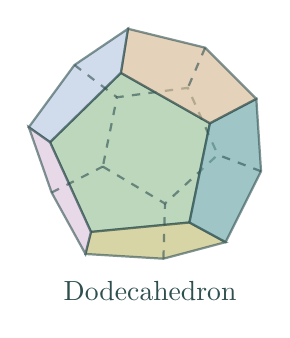
\begin{tikzpicture}[thick,scale=0.5,DarkSlateGray]
    \coordinate (A) at (0,0);
    \coordinate (B) at (2.5,0.24);
    \coordinate (C) at (3.02,2.76);
    \coordinate (D) at (0.76,4.04);
    \coordinate (E) at (-1.04,2.28);
    \coordinate (A1) at (0.3,1.66);
    \coordinate (B1) at (1.88,0.72);
    \coordinate (C1) at (3.22,1.96);
    \coordinate (D1) at (2.46,3.66);
    \coordinate (E1) at (0.66,3.42);
    \coordinate (B2) at (-.14,-.56);
    \coordinate (C2) at (1.84,-.68);
    \coordinate (D2) at (3.42,-.26);
    \coordinate (B3) at (4.32,1.54);
    \coordinate (C3) at (4.2,3.38);
    \coordinate (D3) at (2.9,4.68);
    \coordinate (B4) at (.94,5.16);
    \coordinate (C4) at (-.42,4.24);
    \coordinate (D4) at (-1.58,2.66);
    \coordinate (F) at (-1,1);
    
    \draw[fill=DarkSeaGreen,opacity=0.6] (A)--(B)--(C)--(D)--(E)--cycle;
    \draw[opacity=0.6,dashed] (A1)--(B1)--(C1)--(D1)--(E1)--cycle;
    \draw[fill=DarkKhaki,opacity=0.6] (A)--(B2)--(C2)--(D2)--(B)--cycle;
    \draw[fill=CadetBlue,opacity=0.6] (B)--(D2)--(B3)--(C3)--(C)--cycle;
    \draw[fill=Tan,opacity=0.6] (C)--(C3)--(D3)--(B4)--(D)--cycle;
    \draw[fill=LightSteelBlue,opacity=0.6] (D)--(B4)--(C4)--(D4)--(E)--cycle;
    \draw[fill=Thistle,opacity=0.6] (E)--(D4)--(F)--(B2)--(A)--cycle;
    \path[opacity=0.6] (B2)--(C2)--(B1)--(A1)--(F)--cycle;
    \draw[opacity=0.6,dashed] (C2)--(B1) (F)--(A1);
    \path[opacity=0.6] (C2)--(D2)--(B3)--(C1)--(B1)--cycle;
    \draw[opacity=0.6,dashed] (B3)--(C1);
    \path[opacity=0.6] (B3)--(C3)--(D3)--(D1)--(C1)--cycle;
    \draw[opacity=0.6,dashed] (D3)--(D1);
    \path[opacity=0.6] (D3)--(B4)--(C4)--(E1)--(D1)--cycle;
    \draw[opacity=0.6,dashed] (C4)--(E1);
%titik dengan ball
%http://tex.stackexchange.com/questions/228946/prevent-shifting-of-shading-center-point-when-using-relative-coordinates
    % \shadedraw[ball color=DarkSlateGray!15!white, draw=DarkSlateGray!50] (A) circle (0.08) ;
    % \shadedraw[ball color=DarkSlateGray!15!white, draw=DarkSlateGray!50](B) circle (0.08);
    % \shadedraw[ball color=DarkSlateGray!15!white, draw=DarkSlateGray!50](C) circle (0.08);
    % \shadedraw[ball color=DarkSlateGray!15!white, draw=DarkSlateGray!50](D) circle (0.08);
    % \shadedraw[ball color=DarkSlateGray!15!white, draw=DarkSlateGray!50](E) circle (0.08);
    % \shadedraw[ball color=DarkSlateGray!15!white, draw=DarkSlateGray!50](F) circle (0.08);
    % \shadedraw[ball color=DarkSlateGray!15!white, draw=DarkSlateGray!50] (A1) circle (0.08) ;
    % \shadedraw[ball color=DarkSlateGray!15!white, draw=DarkSlateGray!50](B1) circle (0.08);
    % \shadedraw[ball color=DarkSlateGray!15!white, draw=DarkSlateGray!50](C1) circle (0.08);
    % \shadedraw[ball color=DarkSlateGray!15!white, draw=DarkSlateGray!50](D1) circle (0.08);
    % \shadedraw[ball color=DarkSlateGray!15!white, draw=DarkSlateGray!50](E1) circle (0.08);
    % \shadedraw[ball color=DarkSlateGray!15!white, draw=DarkSlateGray!50](B2) circle (0.08);
    % \shadedraw[ball color=DarkSlateGray!15!white, draw=DarkSlateGray!50](C2) circle (0.08);
    % \shadedraw[ball color=DarkSlateGray!15!white, draw=DarkSlateGray!50](D2) circle (0.08);
    % \shadedraw[ball color=DarkSlateGray!15!white, draw=DarkSlateGray!50](B3) circle (0.08);
    % \shadedraw[ball color=DarkSlateGray!15!white, draw=DarkSlateGray!50](C3) circle (0.08);
    % \shadedraw[ball color=DarkSlateGray!15!white, draw=DarkSlateGray!50](D3) circle (0.08);
    % \shadedraw[ball color=DarkSlateGray!15!white, draw=DarkSlateGray!50](B4) circle (0.081);
    % \shadedraw[ball color=DarkSlateGray!15!white, draw=DarkSlateGray!50](C4) circle (0.08);
    % \shadedraw[ball color=DarkSlateGray!15!white, draw=DarkSlateGray!50](D4) circle (0.08);
   %
    \node[thick,below=0.5cm] at (1.5,0,0) {Dodecahedron};
\end{tikzpicture}
% Icosphedron
    \tdplotsetmaincoords{60}{100}
    \begin{tikzpicture}[tdplot_main_coords,scale=1,line join=round, scale=0.4, DarkSlateGray]
    \pgfmathsetmacro\a{2}
    \pgfmathsetmacro{\phi}{\a*(1+sqrt(5))/2}
    \path 
    coordinate(A) at (0,\phi,\a)
    coordinate(B) at (0,\phi,-\a)
    coordinate(C) at (0,-\phi,\a)
    coordinate(D) at (0,-\phi,-\a)
    coordinate(E) at (\a,0,\phi)
    coordinate(F) at (\a,0,-\phi)
    coordinate(G) at (-\a,0,\phi)
    coordinate(H) at (-\a,0,-\phi)
    coordinate(I) at (\phi,\a,0)
    coordinate(J) at (\phi,-\a,0)
    coordinate(K) at (-\phi,\a,0)
    coordinate(L) at (-\phi,-\a,0); 
    \draw[dashed, thick]    (B) -- (H) -- (F) 
    (D) -- (L) -- (H) --cycle 
    (K) -- (L) -- (H) --cycle
    (K) -- (L) -- (G) --cycle
    (C) -- (L) (B)--(K) (A)--(K)
    ;

        \draw[thick]
        (A) -- (I) -- (B) --cycle 
        (F) -- (I) -- (B) --cycle 
        (F) -- (I) -- (J) --cycle
        (F) -- (D) -- (J) --cycle
        (C) -- (D) -- (J) --cycle
        (C) -- (E) -- (J) --cycle
        (I) -- (E) -- (J) --cycle
        (I) -- (E) -- (A) --cycle
        (G) -- (E) -- (A) --cycle
        (G) -- (E) -- (C) --cycle
        ; 
        \draw[fill=DarkSeaGreen,opacity=0.6] (A) -- (I) -- (B) --cycle ;
        \draw[fill=DarkKhaki,opacity=0.6]  (F) -- (I) -- (B) --cycle ;
        \draw[fill=Tan,opacity=0.6]  (F) -- (I) -- (J) --cycle;
        \draw[fill=CadetBlue,opacity=0.6]  (F) -- (D) -- (J) --cycle;
        \draw[fill=LightYellow,opacity=0.6]    (C) -- (D) -- (J) --cycle;
        \draw[fill=Thistle,opacity=0.6]   (C) -- (E) -- (J) --cycle;
        \draw[fill=DarkGray,opacity=0.6]  (I) -- (E) -- (J) --cycle;
        \draw[fill=LightSteelBlue,opacity=0.6]     (I) -- (E) -- (A) --cycle;
        \draw[fill=DarkSalmon,opacity=0.6]   (G) -- (E) -- (A) --cycle;
        \draw[fill=LightPink,opacity=0.6]    (G) -- (E) -- (C) --cycle;
           %
        \node[thick,below=1.5cm] at (0.7,0,0) {Icosahedron};
\end{tikzpicture}

    \end{figure}
    %
    \begin{itemize}
        \item In this course, we skip platonic solids (except tetrahedron and cube).
    \end{itemize}
\end{frame}
%%%%%%%%%%%%%%%%%%%%%%%%%%%%%%%%%%%%%%%
%        SLIDE 
%%%%%%%%%%%%%%%%%%%%%%%%%%%%%%%%%%%%%%%
\subsection{Prism}
\begin{frame}[t]{Prism}
    \begin{itemize}
        \item Have two faces which are congruent, parallel. These faces are called \textbf{bases}.
        \item All the other faces are called \textbf{lateral faces}. 
        \item Lateral faces can be either:
        \begin{itemize}
            \item parallelogram (oblique prism)
            \item rectangle (right prism)
        \end{itemize}
    \end{itemize}
    %
    \begin{figure}[H]
        \centering
        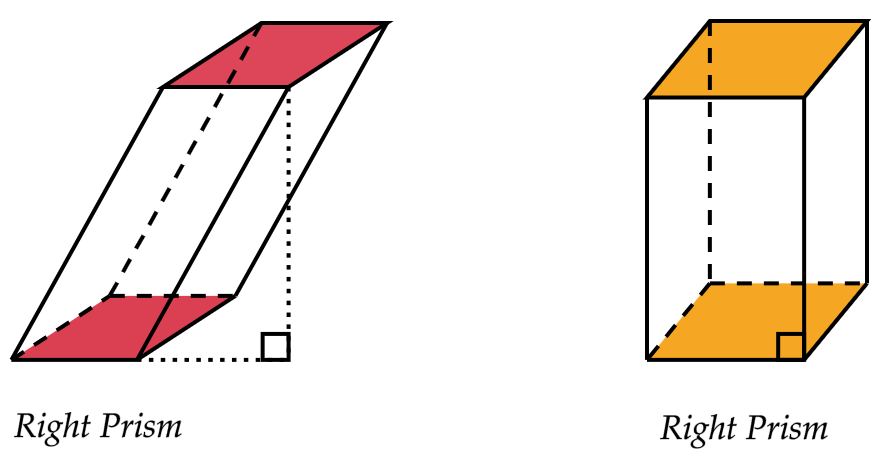
\includegraphics[scale=0.24]{pics/prism.png}
    \end{figure}
    %
    \begin{itemize}
        \item In this course, we only discuss about right prism.
    \end{itemize}
\end{frame}
%%%%%%%%%%%%%%%%%%%%%%%%%%%%%%%%%%%%%%%
%        SLIDE 
%%%%%%%%%%%%%%%%%%%%%%%%%%%%%%%%%%%%%%%
\begin{frame}{Prism (Cont'd)}
    \begin{itemize}
        \item Some examples of right prisms:
    \end{itemize}
    %
    \begin{figure}[H]
        \centering
        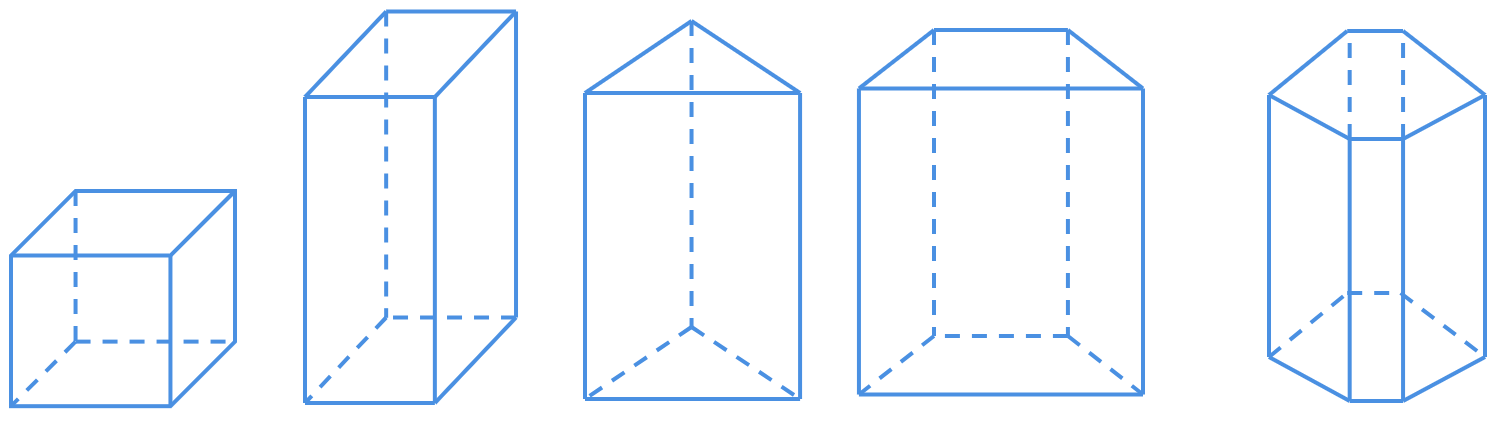
\includegraphics[scale=0.25]{pics/other_prisms.png}
    \end{figure}
\end{frame}
%%%%%%%%%%%%%%%%%%%%%%%%%%%%%%%%%%%%%%%
%        SLIDE 
%%%%%%%%%%%%%%%%%%%%%%%%%%%%%%%%%%%%%%%
\subsection{Pyramid}
\begin{frame}[t]{Pyramid}
    \begin{itemize}
        \item All faces except one intersect at a common vertex.
        \item It has only one base.
    \end{itemize}
    %
    \begin{figure}[H]
        \centering
        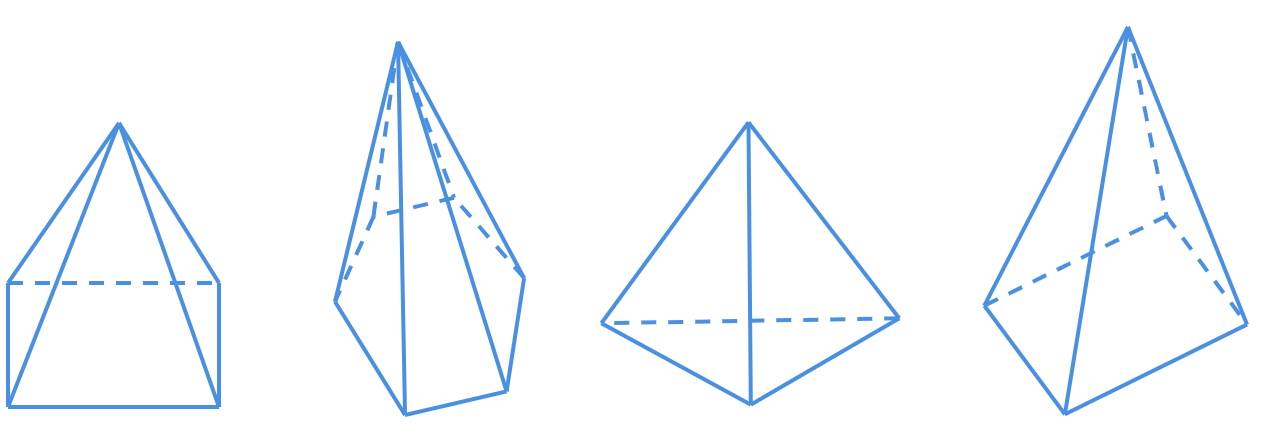
\includegraphics[scale=0.26]{pics/pyramids.png}
    \end{figure}
\end{frame}
%%%%%%%%%%%%%%%%%%%%%%%%%%%%%%%%%%%%%%%
%        SLIDE 
%%%%%%%%%%%%%%%%%%%%%%%%%%%%%%%%%%%%%%%
\section{Volume and Surface Area}
\begin{frame}[t]{Volume and Surface Area}
    \begin{columns}[t]
    \column{0.45\textwidth}
    %
    \boxed{\textbf{Surface Area (SA)}}
    \begin{itemize}
        \item The sum of the areas of all of the faces of a polyhedron.
        \item Surface Area is denoted as SA.
    \end{itemize}
    %
    \begin{figure}[H]
        \centering
        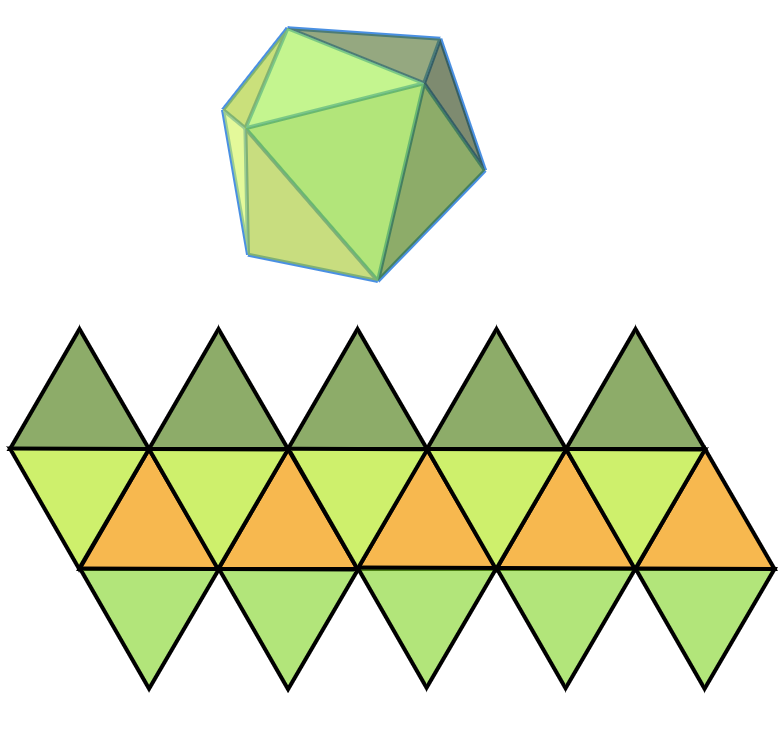
\includegraphics[scale=0.17]{pics/def_surface_area.png}
    \end{figure}
    %
    \column{0.45\textwidth}
    %    
    \boxed{\textbf{Volume ($V$)}}
        \begin{itemize}
            \item The amount of space inside of a shape.
            \item Volume is measured by cubic units. 
        \end{itemize}
    %
    \begin{figure}[H]
        \centering
        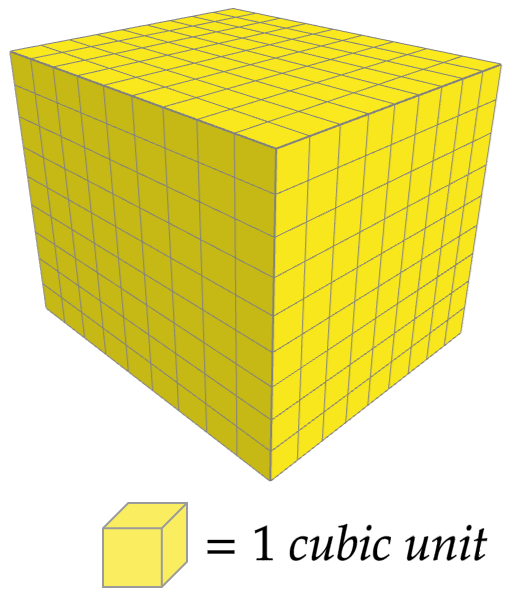
\includegraphics[scale=0.17]{pics/def_volume.png}
    \end{figure}
    %
    \end{columns}
\end{frame}
%%%%%%%%%%%%%%%%%%%%%%%%%%%%%%%%%%%%%%%
%        SLIDE 
%%%%%%%%%%%%%%%%%%%%%%%%%%%%%%%%%%%%%%%
\subsection{Volume and SA of a Prism}
\begin{frame}[t]{Volume and SA of a Prism}
    %
    \begin{columns}[t]
    % SA
    \column{0.45\textwidth}
    \textbf{Surface Area (SA)}
    \begin{itemize}
        \item To find the SA of a prism, you just need to find the area of all faces and add them together.
        \item In this course, we mainly focus on volume of the prism.
    \end{itemize}
    % Volume
    \column{0.45\textwidth}
    \textbf{Volume ($V$)}
    \begin{block}{Formula}
         \[ V = B\cdot h \]
         where $B$ is the area of one base and $h$ is the distance between two bases.
    \end{block}
    \end{columns}
    %
\begin{figure}[H]
    \centering
    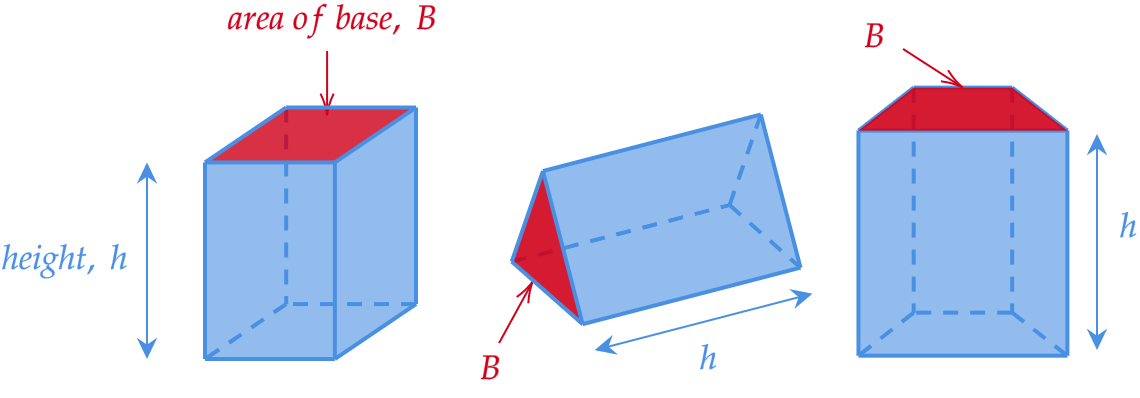
\includegraphics[scale=0.25]{pics/volume_of_prism.png}
\end{figure}
\end{frame}
%%%%%%%%%%%%%%%%%%%%%%%%%%%%%%%%%%%%%%%
%        SLIDE 
%%%%%%%%%%%%%%%%%%%%%%%%%%%%%%%%%%%%%%%
\begin{frame}[t]{Example (Prism)}
    \begin{columns}
        \column{0.45\textwidth}
        \begin{example}
            Find the volume of the prism on the right.
        \end{example}
        %
        \column{0.45\textwidth}
        \begin{figure}[H]
            \centering
            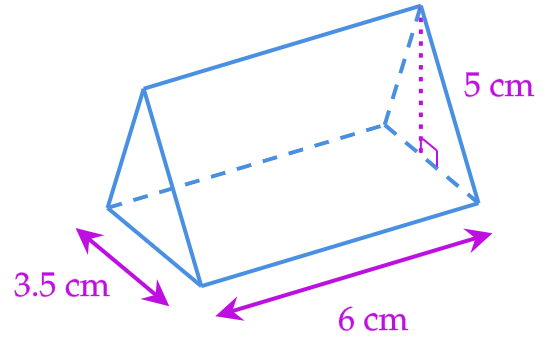
\includegraphics[scale=0.25]{pics/example_volume_prism.png}
        \end{figure}
    \end{columns}
\end{frame}
%%%%%%%%%%%%%%%%%%%%%%%%%%%%%%%%%%%%%%%
%        SLIDE 
%%%%%%%%%%%%%%%%%%%%%%%%%%%%%%%%%%%%%%%
\subsection{Volume and SA of a Pyramid}
\begin{frame}[t]{Volume and SA of a Pyramid}
    %
    \begin{columns}[t]
    % SA
    \column{0.45\textwidth}
    \textbf{Surface Area (SA)}
    \begin{itemize}
        \item Similar to prism, to find SA of a pyramid, just add up the areas of all faces.
        \item In this course, we will work on its volume.
    \end{itemize}
    % Volume
    \column{0.45\textwidth}
    \textbf{Volume ($V$)}
    \begin{block}{Formula}
         \[ V = \frac{B\cdot h}{3} \]
         where $B$ is the area of a base and $h$ is the distance from the common vertex to base.
    \end{block}
    \end{columns}
    %
\begin{figure}[H]
    \centering
    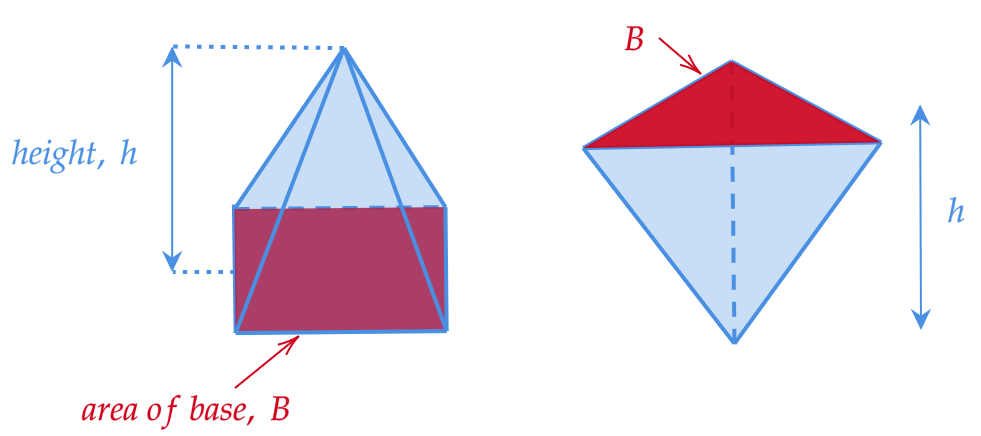
\includegraphics[scale=0.22]{pics/volume_of_pyramid.png}
\end{figure}
\end{frame}
%%%%%%%%%%%%%%%%%%%%%%%%%%%%%%%%%%%%%%%
%        SLIDE 
%%%%%%%%%%%%%%%%%%%%%%%%%%%%%%%%%%%%%%%
\begin{frame}[t]{Example (Pyramid}
    \begin{columns}[c]
        \column{0.45\textwidth}
        \begin{example}
            Find the volume of the pyramid on the right.
        \end{example}
        %
        \column{0.45\textwidth}
        \begin{figure}[H]
            \centering
            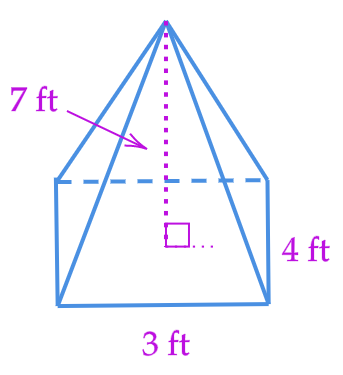
\includegraphics[scale=0.25]{pics/example_volume_pyramid.png}
        \end{figure}
    \end{columns}    
\end{frame}
%%%%%%%%%%%%%%%%%%%%%%%%%%%%%%%%%%%%%%%
%        SLIDE 
%%%%%%%%%%%%%%%%%%%%%%%%%%%%%%%%%%%%%%%
\subsection{Volume and SA of a Rectangular Cube}
\begin{frame}[t]{Volume and SA of a Rectangular Cube (Box)}
    %
    \begin{columns}[t]
    % SA
    \column{0.45\textwidth}
    \textbf{Surface Area (SA)}
    \begin{itemize}
        \item SA can be found easily by opening the box and looking at each face.
    \end{itemize}
    %
    \begin{block}{SA Formula}
         \[ SA = 2\ell w+ 2\ell h+ 2wh \]
    \end{block}
    %
    \begin{figure}[H]
        \centering
        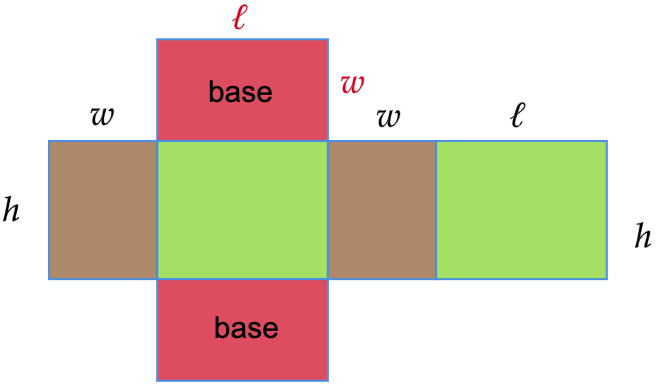
\includegraphics[scale=0.22]{pics/box_SA.png}
    \end{figure}
    % Volume
    \column{0.45\textwidth}
    \textbf{Volume ($V$)}
    %
    \begin{itemize}
        \item We can easily find its volume since it is a prism.
    \end{itemize}
    %
    \begin{block}{Volume Formula}
         \[ V = \ell w h \]
    \end{block}
    %
    \begin{figure}[H]
        \centering
        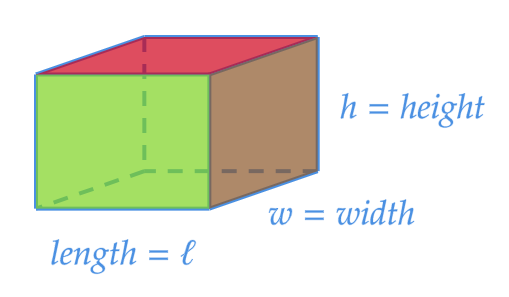
\includegraphics[scale=0.29]{pics/box_volume.png}
    \end{figure}
    \end{columns}
\end{frame}
%%%%%%%%%%%%%%%%%%%%%%%%%%%%%%%%%%%%%%%
%        SLIDE 
%%%%%%%%%%%%%%%%%%%%%%%%%%%%%%%%%%%%%%%
\subsection{Volume and SA of a Cube}
\begin{frame}[t]{Volume and SA of a Cube}
    %
    \begin{columns}[t]
    % SA
    \column{0.45\textwidth}
    \textbf{Surface Area (SA)}
    \begin{itemize}
        \item Cube is a rectangular box in which all sides are equal to $s$.
    \end{itemize}
    %
    \begin{block}{SA Formula}
         \[ SA = 6s^2\]
    \end{block}
    %
    % Volume
    \column{0.45\textwidth}
    \textbf{Volume ($V$)}
    %
    \begin{itemize}
        \item Similar to SA, use the box formula and replace all sides with $s$.
    \end{itemize}
    %
    \begin{block}{Volume Formula}
         \[ V = s^3 \]
    \end{block}
    %
    \end{columns}
    %
    \begin{figure}[H]
        \centering
        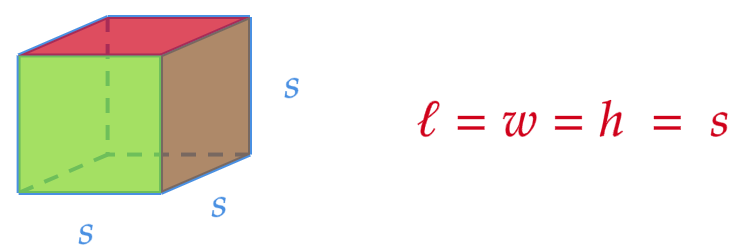
\includegraphics[scale=0.28]{pics/cube_volume.png}
    \end{figure}
\end{frame}
%%%%%%%%%%%%%%%%%%%%%%%%%%%%%%%%%%%%%%%
%        SLIDE 
%%%%%%%%%%%%%%%%%%%%%%%%%%%%%%%%%%%%%%%
\begin{frame}[t]{Example (Cube and Box)}
    \begin{columns}[t]
    %
    \column{0.45\textwidth}
    \begin{example}
        Find the SA and volume of the shapes on the right.
    \end{example}
    %
    \column{0.45\textwidth}
    \begin{figure}[H]
        \centering
        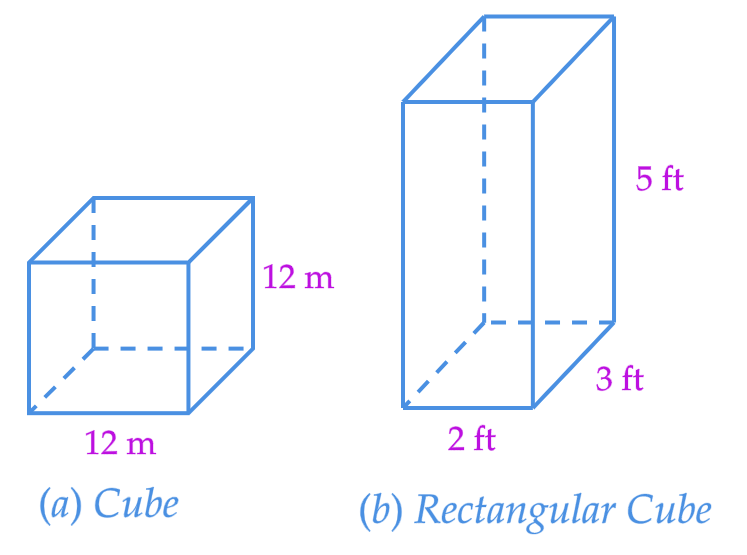
\includegraphics[scale=0.2]{pics/example_cube_box.png}
    \end{figure}
    \end{columns}
\end{frame}
%%%%%%%%%%%%%%%%%%%%%%%%%%%%%%%%%%%%%%%
%        SLIDE 
%%%%%%%%%%%%%%%%%%%%%%%%%%%%%%%%%%%%%%%
\section{Non-Polyhedra Shapes}
\begin{frame}[t]{Non-Polyhedra Shapes}
    \begin{itemize}
        \item We will discuss three shapes that are not polyhedra:
        \begin{itemize}
            \item Cylinder
            \item Cone
            \item Sphere
        \end{itemize}
    \end{itemize}
    %
    \begin{itemize}
        \item Their SA is little bit complicated than polyhedra!
        \item The volume of Cylinder and Cone is like Prim and Pyramid, respectively.
        \item However, the volume of sphere is totally different.
    \end{itemize}
    %
    \begin{figure}[H]
        \centering
        %%%%%%%%%%%%%%%%%%%%
%  Sphere
%%%%%%%%%%%%%%%%%%%%
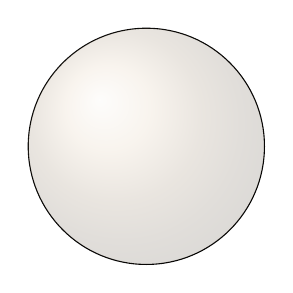
\begin{tikzpicture}[scale=1.5]
    %\draw (-1,0) arc (180:360:1cm and 0.5cm);
    %\draw[dashed] (-1,0) arc (180:0:1cm and 0.5cm);
    %\draw (0,1) arc (90:270:0.5cm and 1cm);
    %\draw[dashed] (0,1) arc (90:-90:0.5cm and 1cm);
    \draw (0,0) circle (1cm);
    \shade[ball color=Tan, opacity=0.20] (0,0) circle (1cm);
\end{tikzpicture}
\hspace{1em}
%%%%%%%%%%%%%%%%%%%%
%  Cone
%%%%%%%%%%%%%%%%%%%%
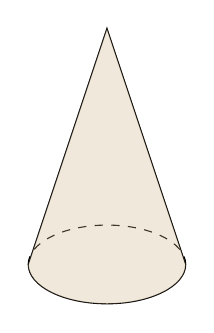
\begin{tikzpicture}
    \draw (-1,0) arc (180:360:1cm and 0.5cm) -- (0,3) -- cycle;
    \draw[dashed] (-1,0) arc (180:0:1cm and 0.5cm);
    \shade[left color=Tan,right color=Tan,opacity=0.3] (-1,0) arc (180:360:1cm and 0.5cm) -- (0,3) -- cycle;
\end{tikzpicture}
%%%%%%%%%%%%%%%%%%%%
\hspace{1em}
%%%%%%%%%%%%%%%%%%%%
%  Cylinder
%%%%%%%%%%%%%%%%%%%%
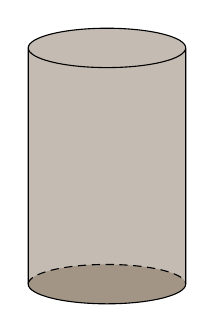
\begin{tikzpicture}[scale=0.5]
    \fill[top color=Tan,bottom color=Tan,middle color=Tan,shading=axis,opacity=0.25] (0,0) circle (2cm and 0.5cm);
    \fill[left color=Tan, right color=Tan,middle color=Tan,shading=axis,opacity=0.25] (2,0) -- (2,6) arc (360:180:2cm and 0.5cm) -- (-2,0) arc (180:360:2cm and 0.5cm);
    \fill[top color=Tan,bottom color=Tan,middle color=Tan,shading=axis,opacity=0.25] (0,6) circle (2cm and 0.5cm);
    \draw (-2,6) -- (-2,0) arc (180:360:2cm and 0.5cm) -- (2,6) ++ (-2,0) circle (2cm and 0.5cm);
    \draw[densely dashed] (-2,0) arc (180:0:2cm and 0.5cm);
\end{tikzpicture}
    \end{figure}
\end{frame}


%%%%%%%%%%%%%%%%%%%%%%%%%%%%%%%%%%%%%%%
%        SLIDE 
%%%%%%%%%%%%%%%%%%%%%%%%%%%%%%%%%%%%%%%
\subsection{Volume and SA of a Cylinder (Right Cylinder)}
\begin{frame}[t]{Volume and SA of a Cylinder}
    \begin{columns}[t]
    % SA
    \column{0.45\textwidth}
    \textbf{Surface Area (SA)}
    \begin{itemize}
        \item The bases of a cylinder are circles.
        \item The area of a lateral face can be found by cutting the cylinder.
    \end{itemize}
    %
    \begin{block}{SA Formula}
         \[ SA = 2\pi r^2 + 2\pi rh\]
    \end{block}
    %
    \begin{figure}[H]
        \centering
        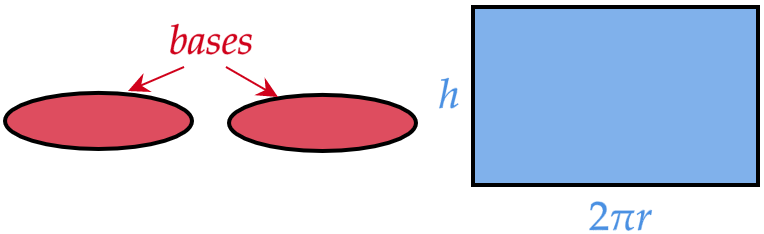
\includegraphics[scale=0.252]{pics/cylinder_SA.png}
    \end{figure}
    % Volume
    \column{0.45\textwidth}
    \textbf{Volume ($V$)}
    %
    \begin{itemize}
        \item Similar to prism, the volume of cylinder is area of a base ($\pi r^2$) times $h$ (distance between two bases).
    \end{itemize}
    %
    \begin{block}{Volume Formula}
         \[ V = \pi r^2 h \]
    \end{block}
    %
    \begin{figure}[H]
        \centering
        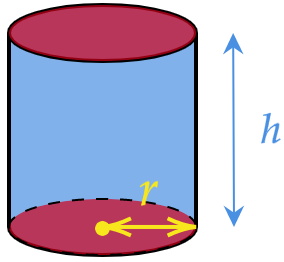
\includegraphics[scale=0.27]{pics/cylinder_v.png}
    \end{figure}
    \end{columns}
    %
\end{frame}
%%%%%%%%%%%%%%%%%%%%%%%%%%%%%%%%%%%%%%%
%        SLIDE 
%%%%%%%%%%%%%%%%%%%%%%%%%%%%%%%%%%%%%%%
\begin{frame}[t]{Example (Cylinder)}
    \begin{columns}[t]
        \column{0.45\textwidth}
        \begin{example}
            Find the surface area and volume of the following cylinder.
        \end{example}
        %
        \column{0.45\textwidth}
        \begin{figure}[H]
            \centering
            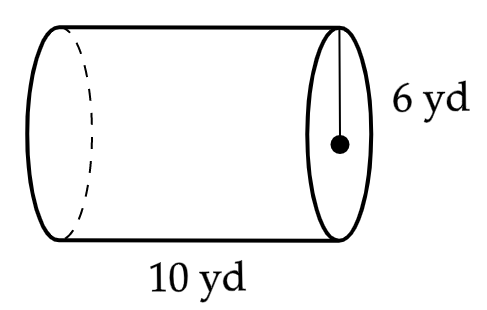
\includegraphics[scale=0.3]{pics/example_cylinder.png}
        \end{figure}
    \end{columns}
\end{frame}
%%%%%%%%%%%%%%%%%%%%%%%%%%%%%%%%%%%%%%%
%        SLIDE 
%%%%%%%%%%%%%%%%%%%%%%%%%%%%%%%%%%%%%%%
\subsection{Volume and SA of a Cone}
\begin{frame}[t]{Volume and SA of a Cone}
    \begin{columns}[t]
    % SA
    \column{0.45\textwidth}
    \textbf{Surface Area (SA)}
    \begin{itemize}
        \item The base of the cone is a circle.
        \item If we cut the cone and open it, we can find its lateral face area.
    \end{itemize}
    %
    \begin{block}{SA Formula}
         \[ SA = \pi r^2 + \pi r \sqrt{r^2+h^2}\]
    \end{block}
    %
    \begin{figure}[H]
        \centering
        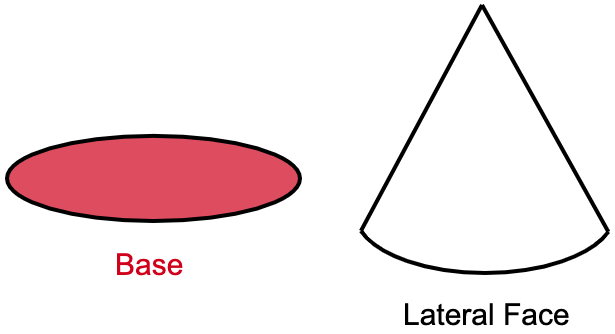
\includegraphics[scale=0.23]{pics/cone_SA.png}
    \end{figure}
    % Volume
    \column{0.45\textwidth}
    \textbf{Volume ($V$)}
    %
    \begin{itemize}
        \item Like pyramid, the volume of cone is one third of the volume of the cylinder with
        same height and radius.
    \end{itemize}
    %
    \begin{block}{Volume Formula}
         \[ V = \frac{\pi r^2 h}{3} \]
    \end{block}
    %
    \begin{figure}[H]
        \centering
        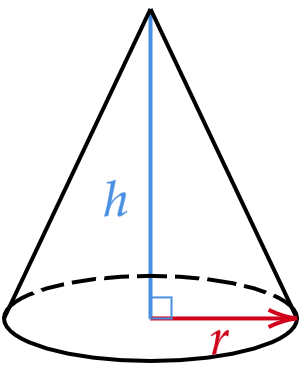
\includegraphics[scale=0.18]{pics/cone_v.png}
    \end{figure}
    \end{columns}
    %
\end{frame}
%%%%%%%%%%%%%%%%%%%%%%%%%%%%%%%%%%%%%%%
%        SLIDE 
%%%%%%%%%%%%%%%%%%%%%%%%%%%%%%%%%%%%%%%
\begin{frame}[t]{Example (Cone)}
    \begin{columns}[t]
    \column{0.45\textwidth}
        \begin{example}
            Find the SA and volume of the following cone.
        \end{example}
    \column{0.45\textwidth}
        \begin{figure}[H]
            \centering
            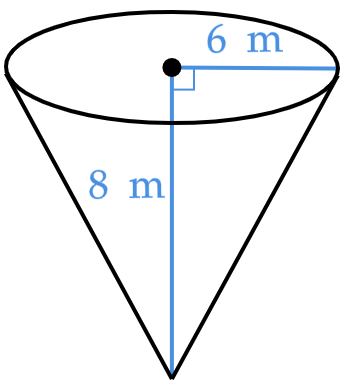
\includegraphics[scale=0.25]{pics/example_cone.png}
        \end{figure}
    \end{columns}
\end{frame}
%%%%%%%%%%%%%%%%%%%%%%%%%%%%%%%%%%%%%%%
%        SLIDE 
%%%%%%%%%%%%%%%%%%%%%%%%%%%%%%%%%%%%%%%
\subsection{Volume and SA of a Sphere}
\begin{frame}[t]{Volume and SA of a Sphere}
    \begin{columns}[t]
    % SA
    \column{0.5\textwidth}
    \footnotesize{
    \begin{itemize}
        \item Archimedes was the first person who discovered the SA and volume of a sphere.
        \item Fitted a cylinder around a sphere.
        \item Cut horizontal slices through the cylinder.
        \item Found the volume between cylinder and sphere.
        \item Then he found the volume of sphere.
        \item Similar technique used to find the SA.
    \end{itemize}}
    %
    \begin{figure}[H]
        \centering
        \input{Tikz/sphere}
    \end{figure}
    \column{0.45\textwidth}
    %
    \begin{block}{SA and Volume Formula}
         \begin{align*}
             SA & = 4 \pi r^2
             \\
             V & = \frac{4\pi r^3}{3}
         \end{align*}
    \end{block}
    %
    \begin{figure}[H]
        \centering
        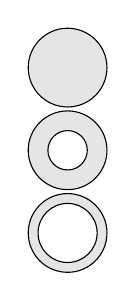
\begin{tikzpicture}[scale=0.5]
    \tikzset{
      reversed with radius/.style={
        x radius=#1,
        y radius=-#1,
     }
    }
    \draw[preaction={fill,opacity=0.1}] (0,0)
      circle[reversed with radius=1cm]
      circle[radius=0.75cm];
     %
     \draw[preaction={fill,opacity=0.1}] (0,2.1)
      circle[reversed with radius=1cm]
      circle[radius=0.5cm];
    %
    \draw[preaction={fill,opacity=0.1}] (0,4.2)
      circle[reversed with radius=1cm];
\end{tikzpicture}
%
%
%%%%%%%%%%%%%%%%%%%%%
% Sphere and Cylinder
%%%%%%%%%%%%%%%%%%%%%
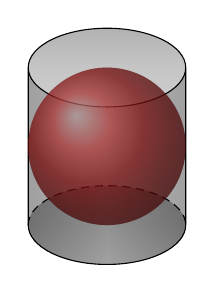
\begin{tikzpicture}
\def\R{1}
  \fill[top color    = gray!50!black,
        bottom color = gray!10,
        middle color = gray,
        shading      = axis,
        opacity      = 0.25]
    (0,0) circle (\R cm and 0.5cm);
  \fill[left color   = gray!50!black,
        right color  = gray!50!black,
        middle color = gray!50,
        shading      = axis,
        opacity      = 0.25]
    (\R,0) -- (\R,2*\R)  arc (360:180:\R cm and 0.5cm)
          -- (-\R,0) arc (180:360:\R cm and 0.5cm);
  \fill[top color    = gray!90!,
        bottom color = gray!2,
        middle color = gray!30,
        shading      = axis,
        opacity      = 0.25]
    (0,2*\R) circle (\R cm and 0.5cm);
  
  \draw (-\R,2*\R) -- (-\R,0) arc (180:360:\R cm and 0.5cm)
              -- (\R,2*\R) ++ (-\R,0) circle (\R cm and 0.5cm);
  \draw[densely dashed] (-\R,0) arc (180:0:\R cm and 0.5cm);
 \fill[thick, ball color=red!90, opacity = 0.5] (0,\R) circle (\R);
% \fill[thick, ball color=orange!90, opacity = 0.5] (0,3*\R) circle (\R);
% \fill[thick, ball color=blue!90, opacity = 0.5] (0,5*\R) circle (\R);
 \end{tikzpicture}
    \end{figure}
    \end{columns}
    %
\end{frame}
%%%%%%%%%%%%%%%%%%%%%%%%%%%%%%%%%%%%%%%
%        SLIDE 
%%%%%%%%%%%%%%%%%%%%%%%%%%%%%%%%%%%%%%%
\begin{frame}[t]{Example (Sphere)}
    \begin{columns}[t]
    \column{0.45\textwidth}
        \begin{example}
            Find the surface area and volume of the golf ball on the right.
        \end{example}
        %
    \column{0.45\textwidth}    
        \begin{figure}[H]
            \centering
            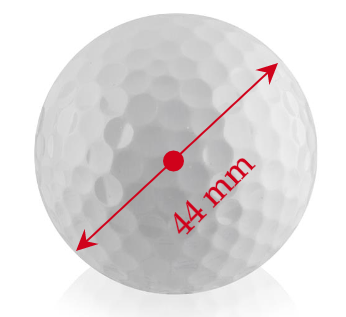
\includegraphics[scale=0.3]{pics/example_golf_ball.png}
        \end{figure}
    \end{columns}
\end{frame}





%%%%%%%%%%%%%%%%%%%%%%%%%%%%%%%%%%%%%%%
%        SLIDE
%%%%%%%%%%%%%%%%%%%%%%%%%%%%%%%%%%%%%%%
\begin{frame}
% \Huge{\centerline{The End}}
\begin{figure}[H]
    \centering
    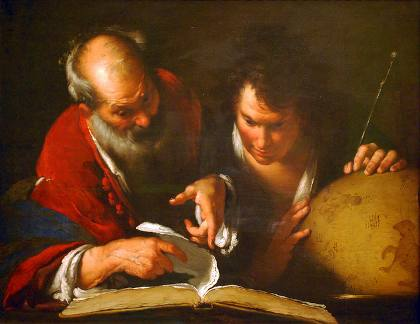
\includegraphics[scale=0.3]{pics/archimedes.jpg}
\end{figure}
\epigraph{Archimedes saw his proof of the volume of a sphere as his greatest personal achievement. His work is remarkable for its similarity to modern calculus. He gave instructions that his proof should be remembered on his gravestone.}%
{ \textit{ 287 BC - 212 BC}}
\end{frame}
%%%%%%%%%%%%%%%%%%%%%%%%%%%%%%%%%%%%%%%
\end{document}